\newgeometry{textwidth=16cm}
\chapter[Phonon calculation]{Network modes identification}
\minitoc
\restoregeometry

\newpage


%-------------------------------------------------------------------------------------------------------------------------
%-------------------------------------------------------------------------------------------------------------------------
%-------------------------------------------------------------------------------------------------------------------------
\section*{Introduction}
\markright{INTRODUCTION}{}
%-------------------------------------------------------------------------------------------------------------------------
%-------------------------------------------------------------------------------------------------------------------------
%-------------------------------------------------------------------------------------------------------------------------

The aim of the present chapter is to perform high-precision quantum mechanical calculations to compute spectra for systems in solid state in order to characterize the signature of the inter molecular vibration for a large variety of aromatic compounds.\\

First, acenes, a family of linear polynuclear aromatic compounds possessing only $\pi-\pi$ interactions \cite{campbell1962crystal,mattheus2001polymorphism,brock1982temperature,facelli1993determination,brock1990temperature}, for which high precision experimental data are available up to pentacene \cite{michaelian2012far}, comprise a first benchmark example of this chapter that illustrates both the potential and the computational challenges found in this line of inquiry.\\

Second, additional calculations were performed for other compounds of the acene family, as well as other systems of the aromatic polycycle molecules family. The aim of these additional calculations is verifying if the position and activity of the network modes identified for the acene molecules in the solid state, and particularly the more active mode, depend on the size, length, the moiety or on the presence of hetero elements of the polycycle system in study.\\



%-------------------------------------------------------------------------------------------------------------------------
%-------------------------------------------------------------------------------------------------------------------------
%-------------------------------------------------------------------------------------------------------------------------
\section{Computational details}
%-------------------------------------------------------------------------------------------------------------------------
%-------------------------------------------------------------------------------------------------------------------------
%-------------------------------------------------------------------------------------------------------------------------


Spectral assignments, determined on the basis of both wavenumber and relative intensity values, has already been made primarily using computed spectra for individual molecules, and dimers \cite{spillebout2014discerning}.
Figure \ref{figure9}, derived from this work, gives a direct comparison of experimental and calculated spectra with our conclusion as for assignment. Unfortunately,in this study both calculations and experiments do not give information about very low-wavenumbers and no real assignment of the inter molecular modes has been achieved. However, this experimental information exist. Far-infrared spectra provide information about intermolecular and inter-ring interactions and about $\pi$-stacking in particular. For example, by using coherent synchrotron radiation it is now becoming possible to make experimental photoacoustic IR measurements in the range 7 to 30 cm$^{-1}$ as demonstrated recently by Billinghurst and Michaelian\cite{billinghurst2010photoacoustic}. Concerning acene, Hineno et al \cite{hineno1975far}  measured spectra of naphthalene and anthracene in the region 190-50 cm$^{-1}$ at liquid helium temperature. In the same way, bands in the experimental vibrational spectra of tetracene and pentacene that cannot be interpreted by Hineno et al based on computed wavenumbers for a single molecule are expected to arise from lattice modes. the failure of these calculations is normal. The accurate description of these network modes requires solid state calculations. In this chapter we propose to use this approach in order to describe these network modes. These calculations were finally carried out with the use of two approaches:\\



First, the calculations were carried out with the projector augmented wave (PAW) implementation of Vienna Ab initio Simulation Package (VASP)\cite{kresse1996efficient}. The generalized gradient approximation (GGA) in the PBE parameterization was considered as the exchange correlational functional \cite{perdew1996generalized}. Structural optimizations (triclinic tetracene crystal) were achieved by setting the convergence criteria for total energies are below $5*10^{-6}$ eV, residual forces to be less than $1*10^{-3}$ eV/Å, and stresses limited to 0.02 GPa. To correct the missing dispersion interactions, we have used several recently proposed methods such as PBE functional with pair potential methods D2, D3 (BJ), TS, and TS+SCS. The details of the implementations and usage of these methods can be found elsewhere \cite{grimme2006semiempirical,grimme2011effect,tkatchenko2009accurate,tkatchenko2012accurate,dion2004van}. To obtain accurate band gaps, we have used the GW approximation \cite{bowman2008variational}.  For getting accurate quasiparticle eigenvalues, we used 200 bands for the summation over the bands in the polarizability and the self-energy formulas, and the polarizability matrices were calculated up to a cutoff  of 500 eV.\\ 

Second, periodic calculations for tetracene were also performed in order to calculated IR intensities with CRYSTAL14 program\cite{dovesi2014crystal14}, using PBE functional and STO-6G (Pople's STO-6G) basis set. Default criteria were used as consider accuracy and SCF convergence. Vibrational frequencies at the $\Gamma$ Point were calculated for the optimized geometry. The empirical dispersion correction by Grimme \cite{grimme2006semiempirical} was performed to take into account weak interactions. \\

 \begin{figure}[H]
 	\centering
 	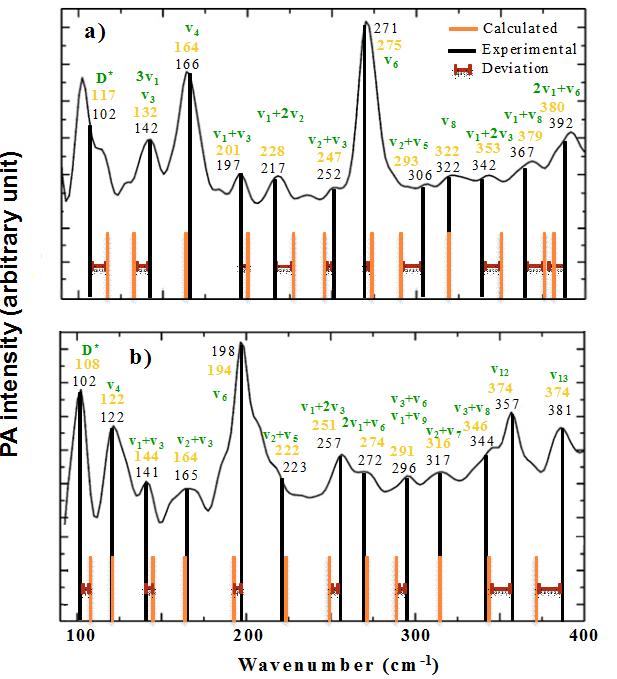
\includegraphics[scale=0.8]{image/final-exp}
 	\caption[Final assignment of the experimental infrared transitions for tetracene and pentacene]{Final assignment of the experimental infrared transitions for a) tetracene and b) pentacene. Calculated wavenumbers are indicated on the spectra with orange lines, and corresponding values above. Experimental values are indicated for comparison, and represented with dark lines} \label{figure9}
 \end{figure}

Only the 0-150 cm$^{-1}$ zone is herein commented in this chapter since it is where the signatures we intend to identify are located. Notwithstanding, for the ensemble of systems, the calculated data were also extended to englobe the 150-400 cm$^{-1}$, allowing in this way both the validation of our calculations in a better experimentally identified zone and the identification of the specific modes of the ‘non interacting’ modes. As such, the solid state calculations herein performed are generally in a very good agreement with the available experimental data. This also contributes to the validation of our results using the same calculation conditions for the regions below 150 cm$^{-1}$.\\




%-------------------------------------------------------------------------------------------------------------------------
%-------------------------------------------------------------------------------------------------------------------------
%-------------------------------------------------------------------------------------------------------------------------
\section{A first case: Tetracene}
%-------------------------------------------------------------------------------------------------------------------------
%-------------------------------------------------------------------------------------------------------------------------
%-------------------------------------------------------------------------------------------------------------------------

We performed first-principle calculations for tetracene in order to clarify its structural and electronic properties of the solid-state system. These calculations strongly suggest the necessity to go beyond the standard DFT approach. First, we have shown that dispersion corrected methods are necessary to provide an improvement in the calculated lattice parameters and volume of the unit cell to compare with experimental values. The complete list of resulting lattice parameters, angles, and volumes along with experimental results for the tetracene compound are presented in Table \ref{table13}. Furthermore, the mean absolute deviations observed for the calculation of these parameters for all the methods under consideration depend on the type of dispersion correction, and the relative errors on structural properties calculated using each method, in particular concerning the volume, may vary significantly. As mentioned by Lebegue et al \cite{appalakondaiah2015dispersion}, it has been demonstrated that one has to test all the dispersion corrected DFT methods for the C-, H-, N- and O- based energetic solids before concluding the ground state properties. Since the D3 correction yields the most accurate structural descriptions of this model system, it has been used to calculate the vibrational, structural and electronic properties.\\
 
 \begin{table}[t]
 	\caption{Lattice parameters of Tetracene molecule calculated in VASP code} \label{table13}
 	\begin{center}
 	\begin{threeparttable}
 		\begin{tabular}{c c c c c c c}
 			\toprule
 			 & \textbf{D2} & \textbf{D3} & \textbf{TS} & \textbf{TS-SCS} & \textbf{PBE*} & \textbf{Exp} ref\cite{campbell1962crystal} \\
 			 \midrule
 			 \textbf{a} &7.54 (7.41) &  7.92 & 7.71 & 7.70 & 9.25 & 7.90\\
 			 \textbf{b}& 5.96 (5.83) & 6.00 & 5.99 & 6.08 & 7.21 & 6.03 \\
 			 \textbf{c}& 13.28 (13.39) & 13.38 & 13.38 & 13.47 & 16.62 & 13.53 \\
 			 \textbf{$\alpha$} & 102.10 (102.21) & 101.21 & 101.36 & 100.97 & 101.36 &100.30\\
 			 \textbf{$\beta$} & 114.33 (113.23) & 113.26 & 113.61 & 114.39 & 112.14 & 113.20\\
 			 \textbf{$\gamma$} &85.20 (85.11) & 85.89 & 85.74 & 85.68 & 86.67 & 86.30\\
 			 \textbf{Volume ($\AA^{3}$)} & 531.41 (519.01) & 572.96 & 554.74 &  563.74 & 1007.16 & 582.85\\
 			 \bottomrule
 		\end{tabular} 
 		
 		\begin{tablenotes}
 			\item[*] without dispersion correction
 			\item[()] Parenthesis values were calculated with CRYSTAL program
 		\end{tablenotes}
 	\end{threeparttable}
 	\end{center}
 \end{table}
 
 \begin{figure}[h]
 	\centering
 	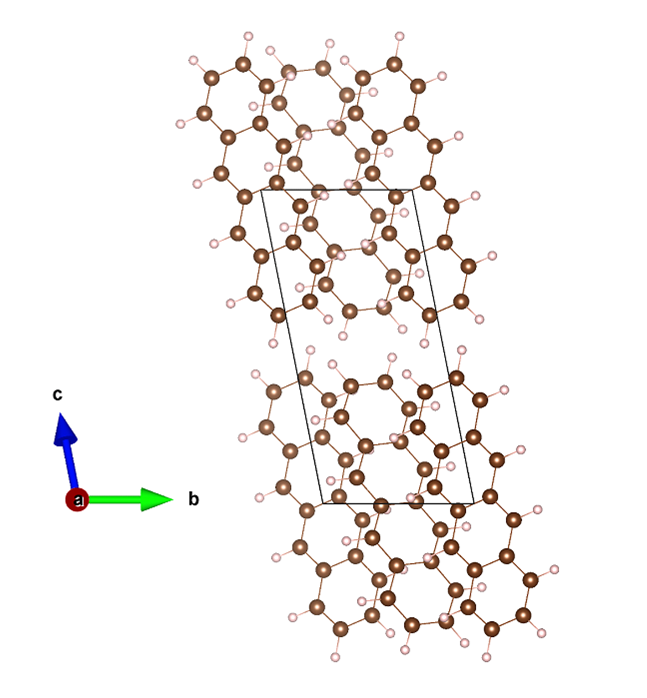
\includegraphics[scale=0.6]{image/T-a}
 	\caption{The \textit{bc} plane of Tetracene Crystal}  \label{tetra-crystal-a}
 \end{figure}
 
 \begin{figure}[h]
 	\centering
 	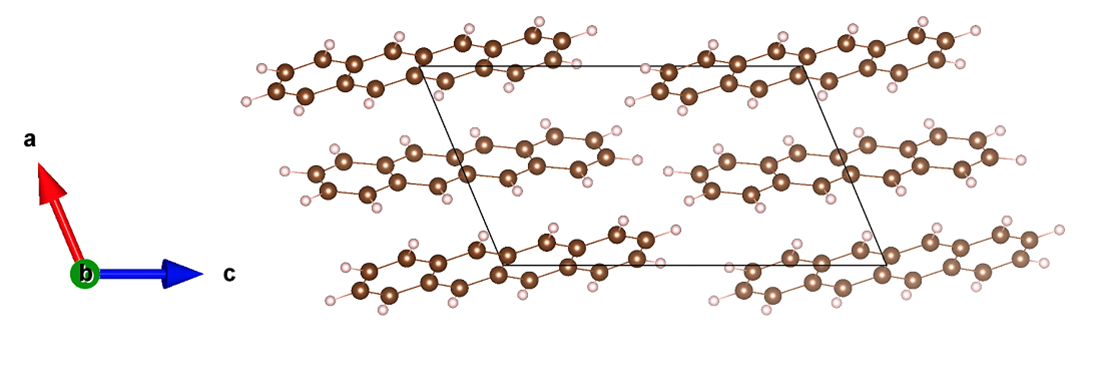
\includegraphics[scale=0.6]{image/T-b}
 	\caption{The \textit{ac} plane of Tetracene Crystal} \label{tetra-crystal-b}
 \end{figure}
 
 \begin{figure}[h]
 	\centering
 	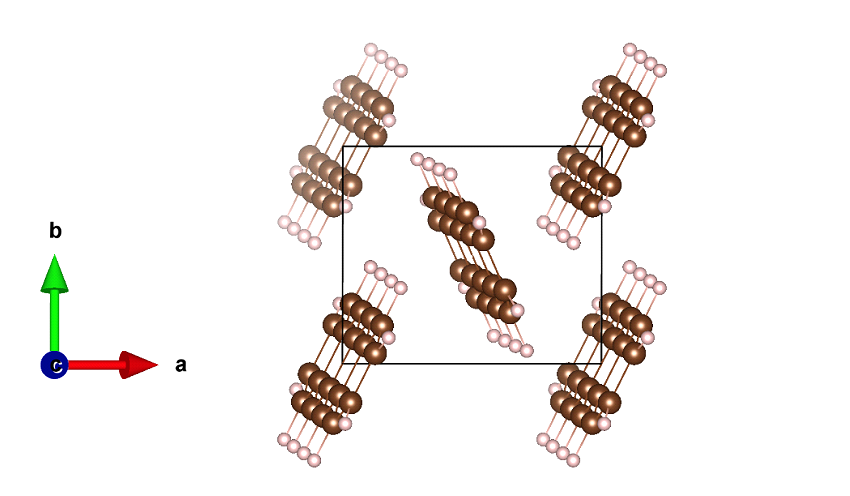
\includegraphics[scale=0.6]{image/T-c}
 	\caption{The \textit{ab} plane of Tetracene Crystal}  \label{tetra-crystal-c}
 \end{figure}
 
 Table \ref{table14} reports all the results obtained for tetracene, from the isolated up to the solid-state system. Beyond the numerical differences due to the various Hamiltonians used for these calculations, the results show significant differences on both vibration frequencies and intensities that are to be attributed to the effect of the chemical environment. Indeed, the signatures of some particular modes (such as $\nu_{2}$ and $\nu_{8}$) are modified with respect to the isolated system due to intermolecular interactions. Besides, our previous study on tetracene dimers revealed that intermolecular interactions induced the appearance of some characteristic spectral signatures at very low wavenumbers. For instance, the mode experimentally found at 106 cm$^{-1}$, which has been assigned, with aid of calculations, to a libration mode, is part of the characteristic signatures of intermolecular vibrations of acenes; the same mode was also assigned at 102 cm$^{-1}$ for the pentacene system in our previous work. In fact, this mode cannot be only associated to a dimer: it results from the vibrations of the whole tetracene molecules within the network that constitutes the aggregate or the cristalline system. Our VASP calculations clearly show that this vibration mode is linked to distortions of the  crystalline network, which can be seen as the « breathing » of the network. Such a deformation was already partially taken into account in the study of a dimer. Some other modes of the crystalline network constitute, to a lesser extent, the remaining characteristic signatures of the intermolecular vibrations. More difficult to detect experimentally, these modes are theoretically found at 69.7 cm$^{-1}$ ($\nu_{1}$), 128.5 cm$^{-1}$ ($\nu_{3}$) and 320.8-323.8 cm$^{-1}$ ($\nu_{8}$). Unfortunately, there is no experimental data available below 100 cm$^{-1}$ for the tetracene system. But it seems that the $\nu_{3}$ and $\nu_{8}$ modes can now be identified as the modes of medium intensity reported from experimental data at 142 and 322 cm$^{-1}$, respectively. Not fundamental mode nor combination mode of the isolated tetracene can be associated with the presence of those new experimental signatures.
 
 From all the modes calculated between 200-400 cm$^{-1}$, whatever their intensities are, they do not seem to be coupled to the vibration of the crystalline network. It suggests that calculations of the isolated molecule (or its dimer) are a sufficient approximation to identify these vibration modes. In the present case, it explains the fact that no assignation problem was found for regions beyond 200 cm$^{-1}$ during the molecular study of tetracene and its dimer.


The tetracene molecule is a favorable case to detect the network signature. Indeed, as indicated in Table \ref{table14}, the isolated tetracene molecule strictly owns a single signature in the zone of study (93 cm$^{-1}$) that could potentially hide the network’s one. Nevertheless, as the intensity of this mode for the monomer is expected to be zero accordingly to our calculations, one should not have problems assigning it. This situation is very favorable and does not represent the most common situation. Occasional overlap of vibrators could be a limiting factor for our capability to identify the nature of these observed vibrators in some cases. Still, this fact does not question the presence of these active network modes that we intend to identify, neither the fact that these modes can always be associated to one or two intra molecular vibrations. \\

 
 To conclude, the use of a model able to describe the chemical environment was essential to identify the spectral signatures of the inter-molecular modes that we try to characterize in our study of asphaltenes (or, at least, of acenes systems). The calculated phonon spectrum thus seems to answers, even if our calculations up to now do not account for both mechanical and electrical anharmonicities. Such conditions are all the more necessary for an exhaustive study of the modes of each isolated molecule. Particularly, it allows an identification of the combination modes as well as the harmonics for which the signatures have been clearly evidenced by photo-acoustic measurements. Only a double approach (both molecular and solid-state) can allow one to completely identify the spectroscopic results of acenes molecules in the crystalline state.
 
 \begin{table}[H]
 	\singlespacing
 	\caption{ Calculated vibrational frequencies (cm$^{-1}$) of the monomer, dimer and solid-state (PBE tetracene system).} \label{table14}
 	\begin{center}
 		\begin{threeparttable}
 		\begin{tabular}{c c c c c}
 			\toprule
 			\multicolumn{2}{p{4.5cm}}{\centering \textbf{Monomer}} & \textbf{Dimer} & \multicolumn{1}{p{4cm}}{\centering \textbf{Experimental} \\ \textbf{(P.A.) this work}} & \textbf{VASP/CRYSTAL}\\
 			Assignment & $\nu$(cm$^{-1}$) & $\nu$(cm$^{-1}$) & $\nu$(cm$^{-1}$) & $\omega$(cm$^{-1}$) \\
 			& Int(km/mol) & Int(km/mol) & & Int(relative) \\
 			\midrule
 			& & \textit{15 (<0.01)} & & \\
 			& & \textit{31 (0)} & & \\
 			& & \textit{52 (0)} & & \\
 		   $\nu_{1}$& 57 (0.8) & 59 (0.6) &  & 69.7 (8.2) \\
 		   & & \textit{80 (1.0)} & & \\
 		   & & \textit{87 (0.1)} & & \\
 		  & & 94 (0) & & \\
 		  & & 112 (0) & & \\
 		  $\nu_{2}$ & 93 (0) & 117 (0.3) & 106 (m) + sh & \multicolumn{1}{p{4cm}}{\centering 102.4 (2.1) \\ \textit{105.7 (9.5)}}\\
 		  & & 124 (0) & & \\
 		  3$\nu_{1}$& 132 (<0.01) & & & \\
 		  $\nu_{3}$& 153 (0.01) &  & 142 (m) & \multicolumn{1}{p{4cm}}{\centering 128.5 (7.1) \\ 148 (0.1)}\\ 
 		  & & 162 (0)&  & \\
 		  $\nu_{4}$& 164 (1.3) & 168 (1.7) & 166 (s) + sh & 164.6 (15.5) \\
 		  & & 169 (0) & & \\
 		  $\nu_{5}$ & 199 (0.05) & 176 (0.2) & 197 (w) & 170.1 (0.1) \\
 		  $\nu_{1}+\nu_{3}$ & 201 (<0.01) &  &  & \\
 		  & & 208 (0) & & \\
 		  &  & 212 (0.09) & 217 (w) & \\
 		  $\nu_{1}+ 2\nu_{2}$ & 228 (<0.01) & & & \\
 		  $\nu_{2}+\nu_{3}$& 247 (0.01) &  & 252 (vw) & \\
 		  $\nu_{6}$ & 275 (1.03) & 282 (1.6) & 271 (m) & 267.4 (3.0)\\
 		  	&  & 286 (0) &  & 274.6 (2.6)\\
 		  	$\nu_{2}+ \nu_{5}$ & 293 (<0.01) &  & 306 (vw) & \\
 		  	& & 316 (0) & & \\
 		   & & 316 (0.03) & & \\
 		    &  & 324 (0) & 322 (w) & 320.8 (0.9)\\
 		    $\nu_{8}$& 322 (<0.01) & 325 (0.06) & & 323.8 (0.5)\\
 		    &  & 335 (0.03) & 342 (w) & \\
 		    & & 335 (0) & & \\
 		    $\nu_{1}+ 2\nu_{3}$ & 353 (<0.01) & &  & \\	
 		    $\nu_{1}+ \nu_{8}$ & 379 (<0.01) & & & \\
 		    $\nu_{10}$ & 385 (0.04) & 390 (0.02) &  392 (m) & \\
 		    2$\nu_{1}+ \nu_{6}$ & 380 (<0.01) &  & & \\
 		    \bottomrule	    
 		  \end{tabular}
 		  
 		  \begin{tablenotes}
 		  	\item[] Italic: Intermolecular modes
 		  \end{tablenotes}
 		\end{threeparttable}
 	\end{center}
 \end{table}
 






%-------------------------------------------------------------------------------------------------------------------------
%-------------------------------------------------------------------------------------------------------------------------
%------------------------------------------------------------------------------------------------------------------------- 
\section{Impact of the chain-length parameter on the vibrational signature of the crystalline network.}
%-------------------------------------------------------------------------------------------------------------------------
%-------------------------------------------------------------------------------------------------------------------------
%-------------------------------------------------------------------------------------------------------------------------

 
 We are aware that it is not possible to jump to conclusions on the basis of the results of a single system. In the same way, additional calculations were performed within this work for other compounds of the acene family, as well as other systems of the aromatic polycycle molecules family. The aim of these additional calculations is verifying if the position and activity of the network modes identified for the tetracene molecule, and particularly the mode clearly localise at around 106 cm$^{-1}$, depend on the size, length or on the moiety of the polycycle system in study.\\
 
 The first parameter we studied is the chain-length within the acene family. A series of calculations on the benzene, naphthalene, anthracene and pentacene calculations was performed. The crystalline structures from which we were able to do our calculation are presented hereafter. More particularly, the benzene molecule has three different phases: Phase I correspond to an orthorhombic Pbca space group that contain four molecules per unit cell. In opposite, the two other phases called II and III contain two molecules in the unit cell and crystallizes in a monoclinic system (space group P21/c) at high pressure \cite{meijer1996density,katrusiak2010association}. In that case molecule configuration observed by differents study is T-Shape \cite{katrusiak2010association}. Under ambient conditions of temperature and under low-pressure, crystals of the naphthalene belong to the monoclinic system (space group P21/a) and contain two molecules per unit cell \cite{fabbiani2006exploration}. Under the same conditions, the crystals of both anthracene and tetracene crystallize in a monoclinic phase P21/a \cite{brock1990temperature} and in a triclinic phase P\={1} \cite{sondermann1985x} respectively. Crystals of the pentacene system crystallize into a triclinic phase (space group P\={1}); it is reported to have two polymorphs structures in its bulk phase, polymorph C \cite{campbell1961crystal} and polymorph H \cite{mattheus2001polymorphism}. The ensemble of the numerical results relative to the cell parameters and cell volumes can be found in Tables \ref{table-benzsol}-7. A representation of these crystalline cells is given in Figures \ref{fig-benzsol}-8.
 
 \begin{figure}[H]
 \begin{center}
 	\resizebox{20cm}{!}{
 	\begin{tabular}{c c}
 	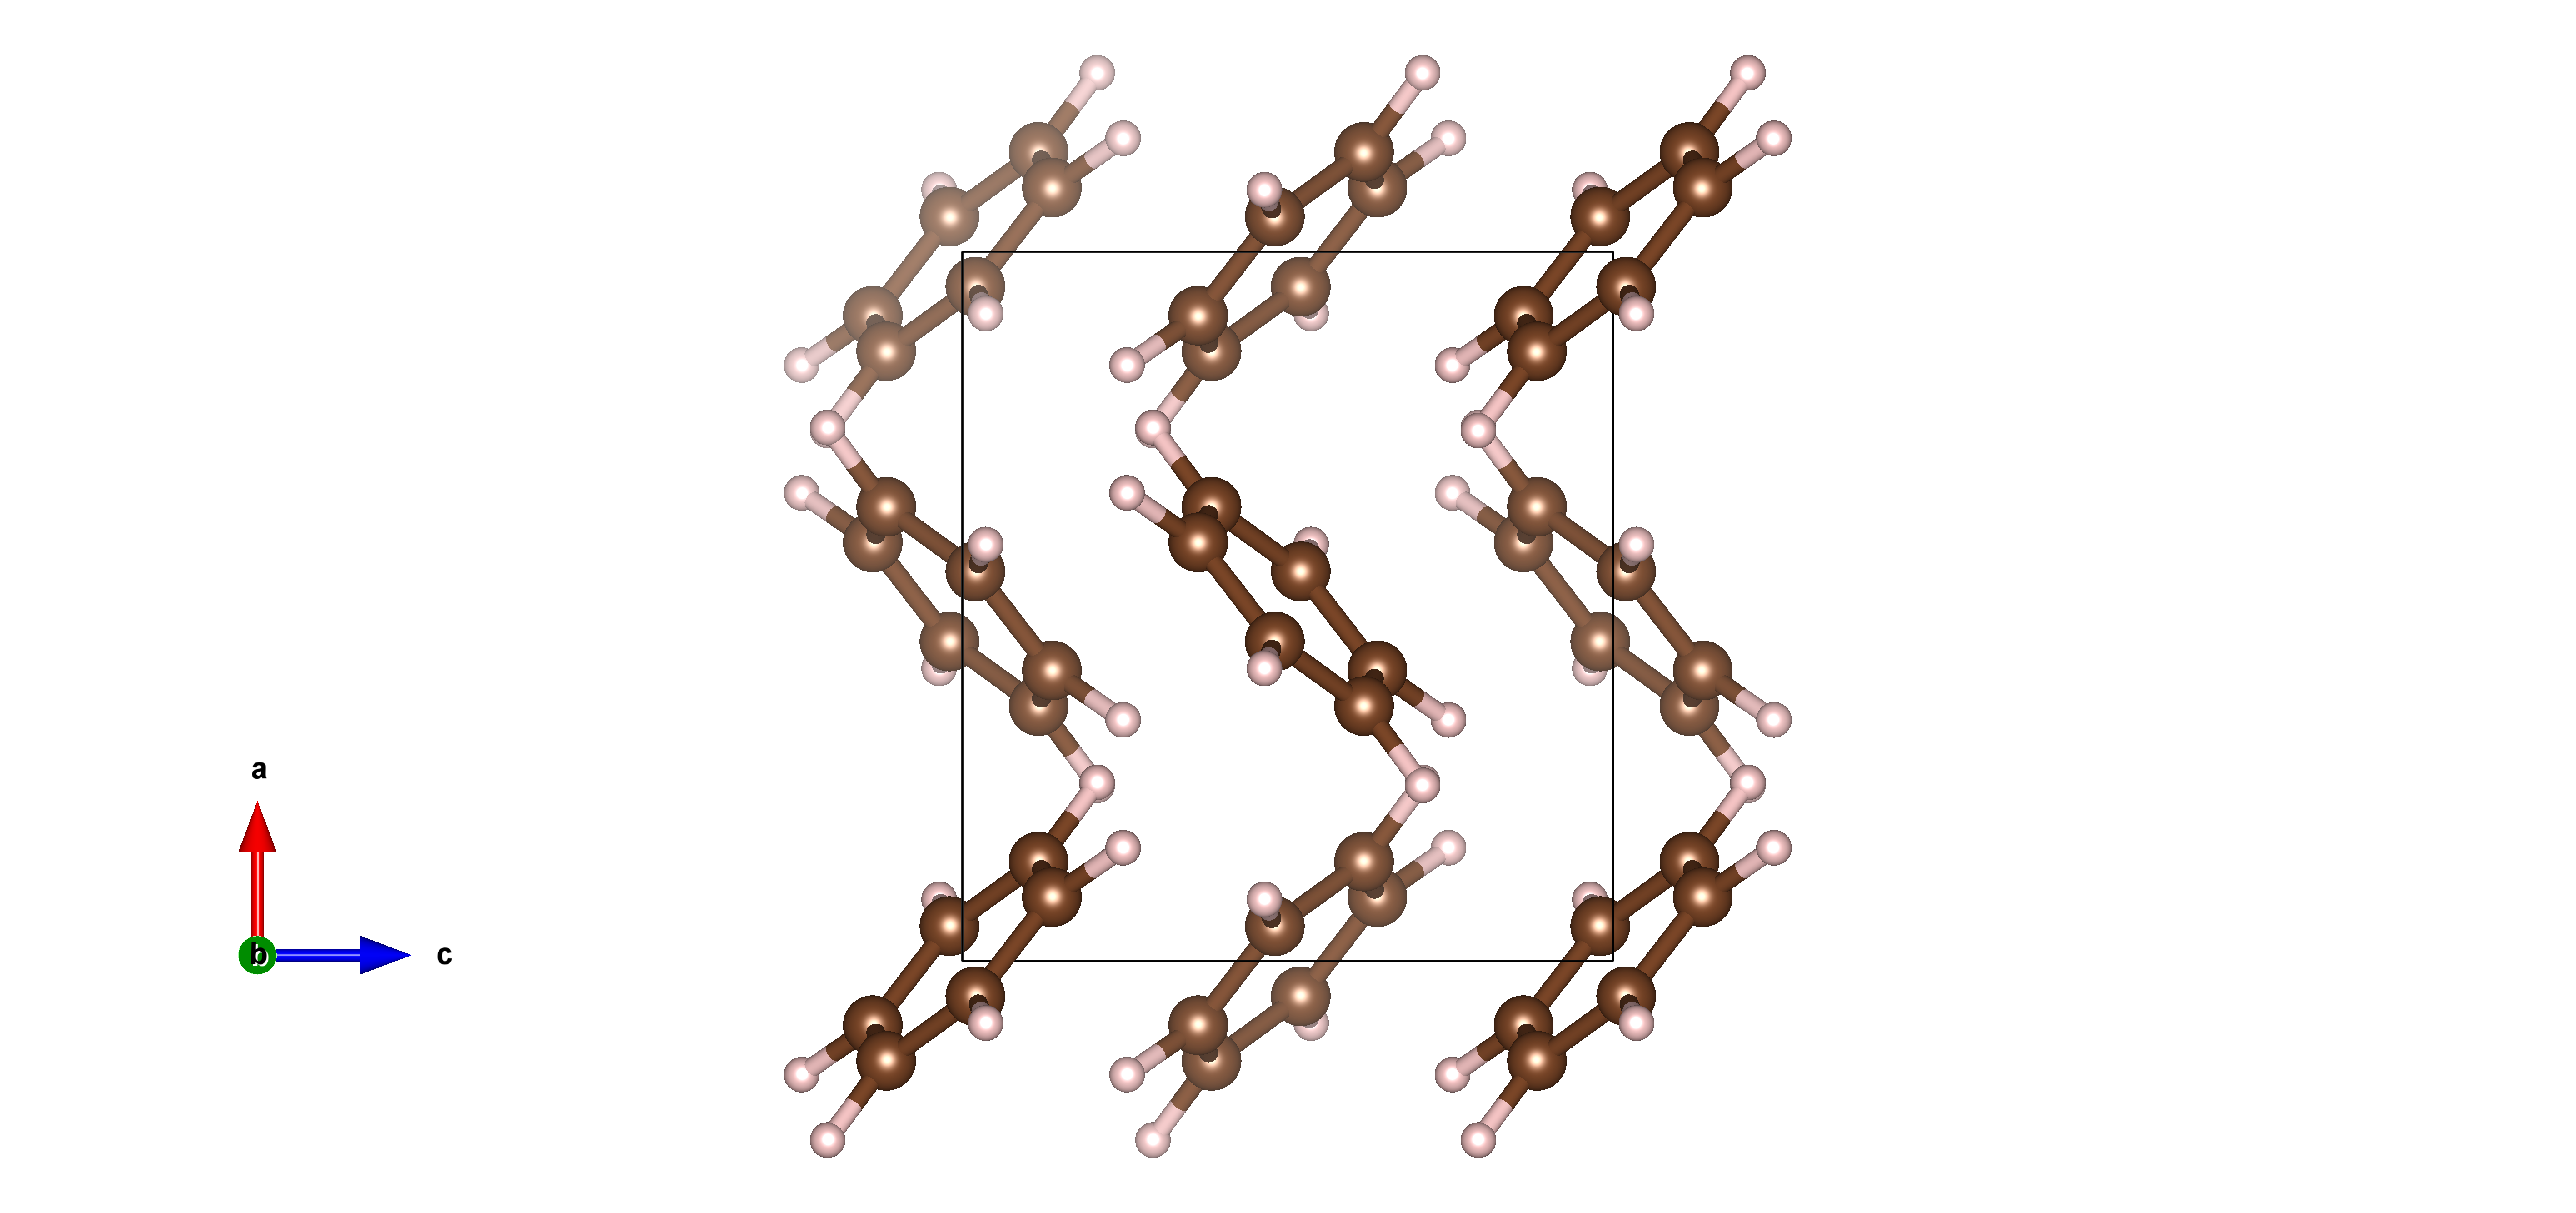
\includegraphics[scale=0.5]{image/Benzene-b} & 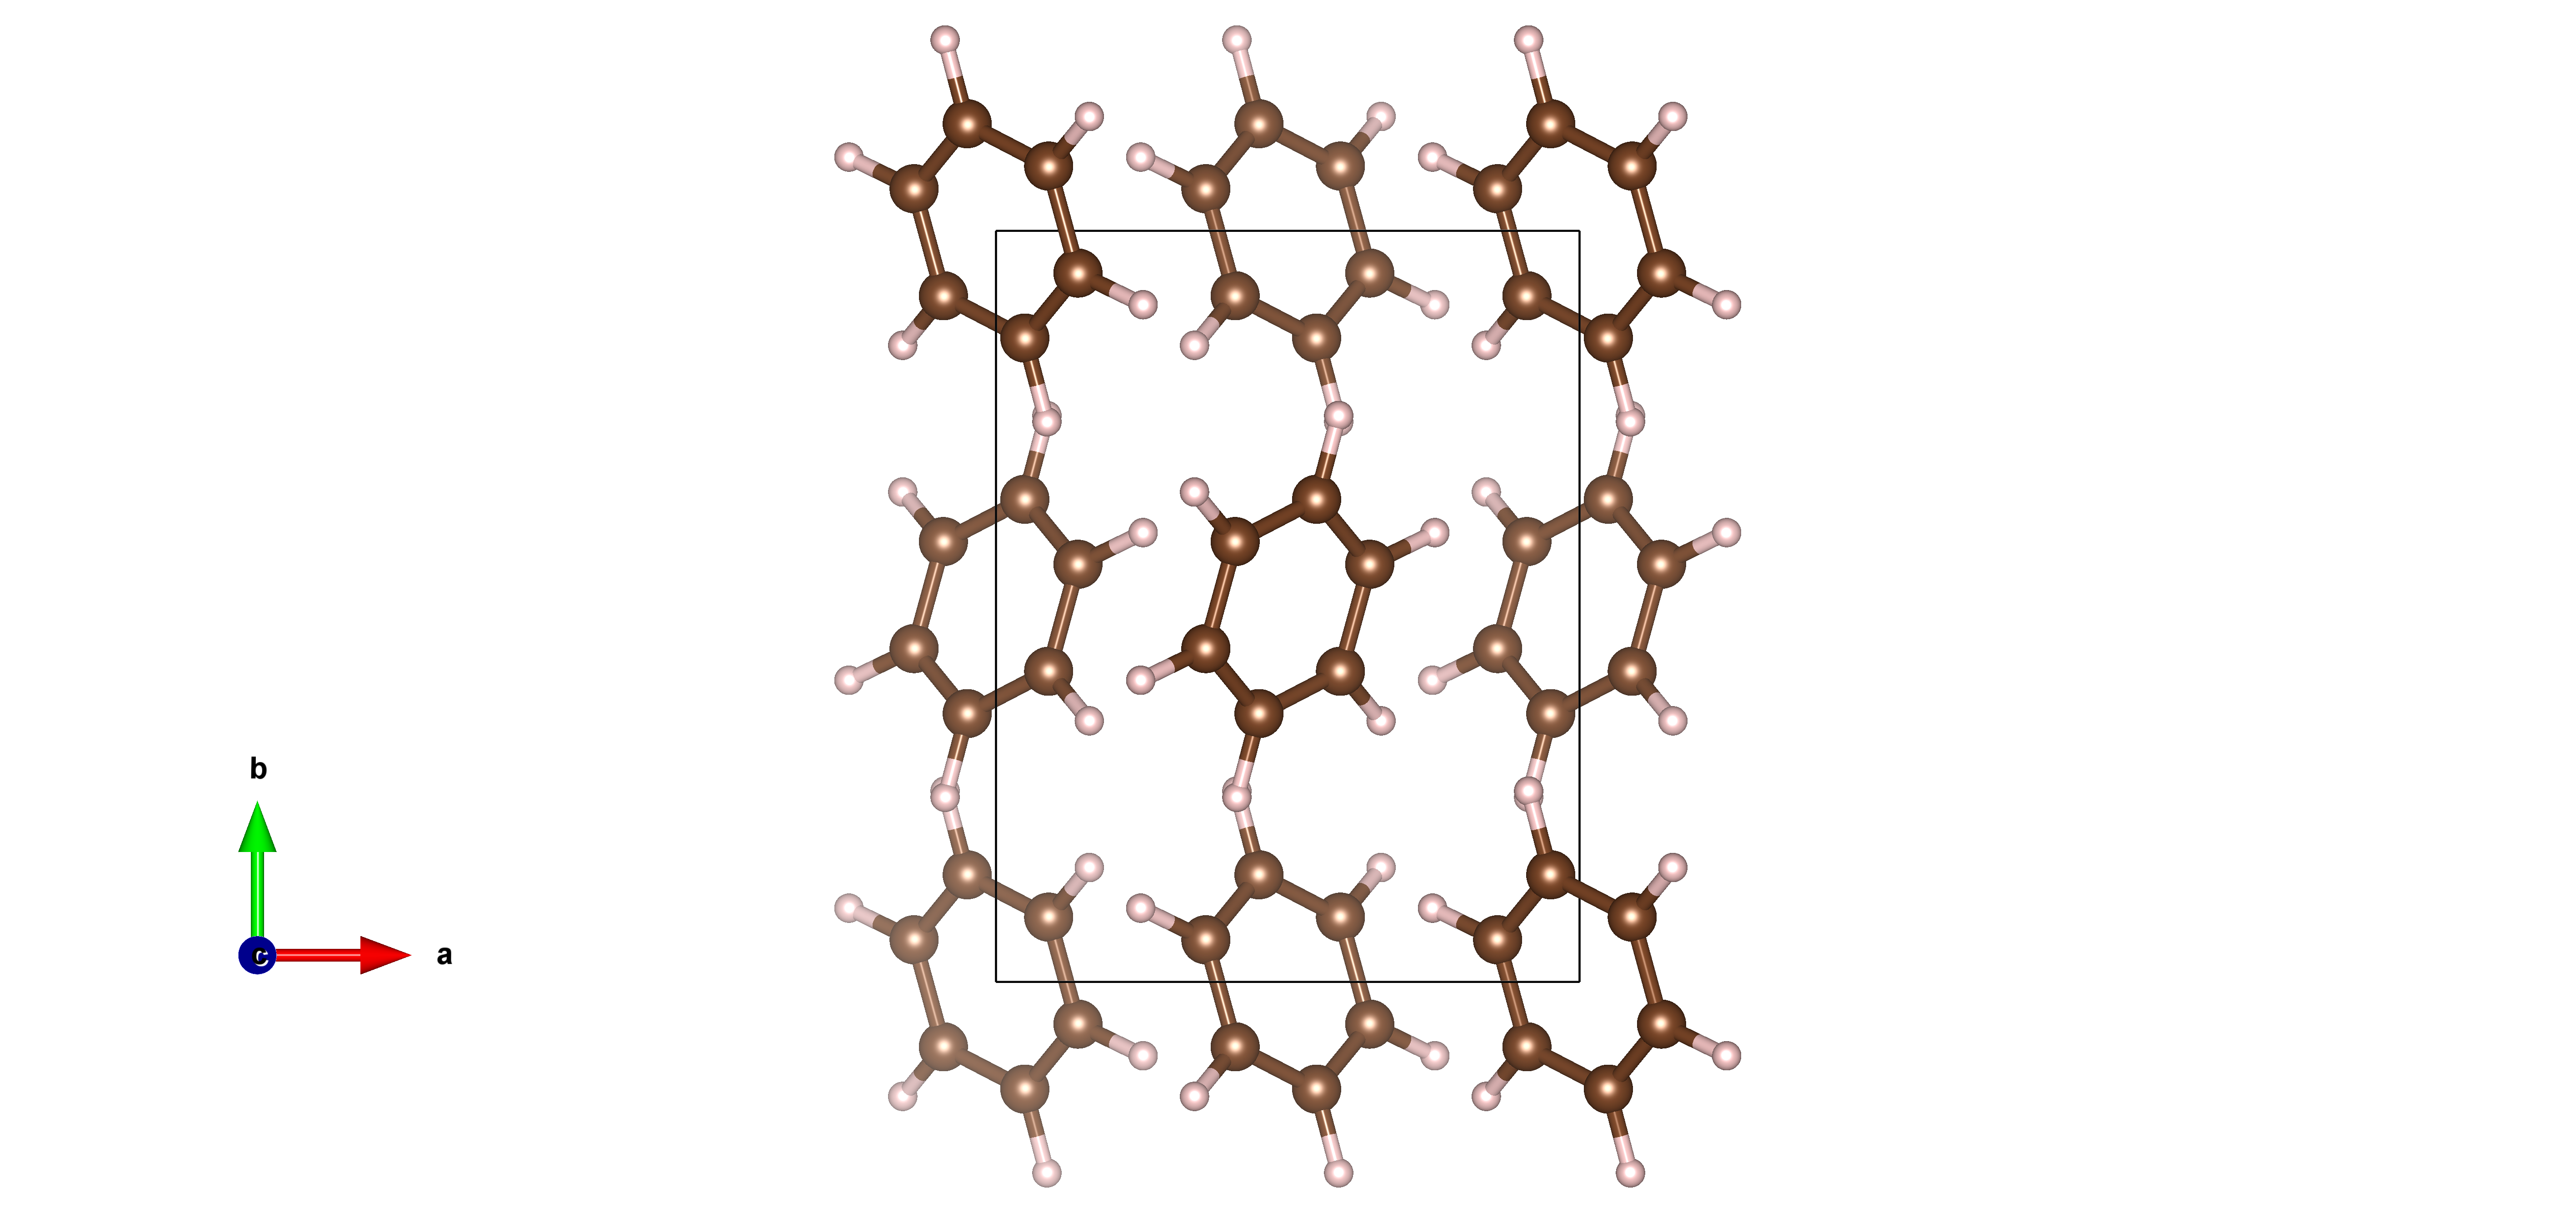
\includegraphics[scale=0.5]{image/Benzene-c} \\	
 	\end{tabular}}
 	\caption{The \textit{ac} and \textit{ab} planes of Benzene crystal}  \label{fig-benzsol}
 \end{center}
  \end{figure}
 
 	 	
 	
 	\begin{table}[H]
 		\caption{Lattice parameters of Benzene molecule calculated in VASP code} \label{table-benzsol}
 		\begin{center}
 			\begin{threeparttable}
 			\begin{tabular}{c c c c c c c}
 				\toprule
 				& \textbf{D2} & \textbf{D3} & \textbf{TS} & \textbf{TS-SCS} & \textbf{PBE*} & \textbf{Exp} ref\cite{meijer1996density} \\
 				\midrule
 				\textbf{a} &7.24 (6.90)& 7.45 & 7.32 & 7.33  & 8.29 & 7.36\\
 				\textbf{b}& 9.09 (9.13) & 9.54 & 9.41 & 9.42 & 10.35 & 9.37\\
 				\textbf{c}& 6.63 (6.55) & 6.84 & 6.71 & 6.72 & 7.73 & 6.70 \\
 				\textbf{Volume ($\AA^{3}$)}& 434.57 (412.45) & 485.94& 462.14 & 463.15 & 662.85 & 465.60\\
 				\bottomrule
 			\end{tabular}
 			
 			\begin{tablenotes}
 				\item[*] without dispersion correction
 				\item[()] Parenthesis values were calculated with CRYSTAL program
 			\end{tablenotes}
 		\end{threeparttable}
 		\end{center}
 	\end{table}
 
 
 \begin{figure}[H]
 	\begin{center}
 		\resizebox{20cm}{!}{
 			\begin{tabular}{c c}
 			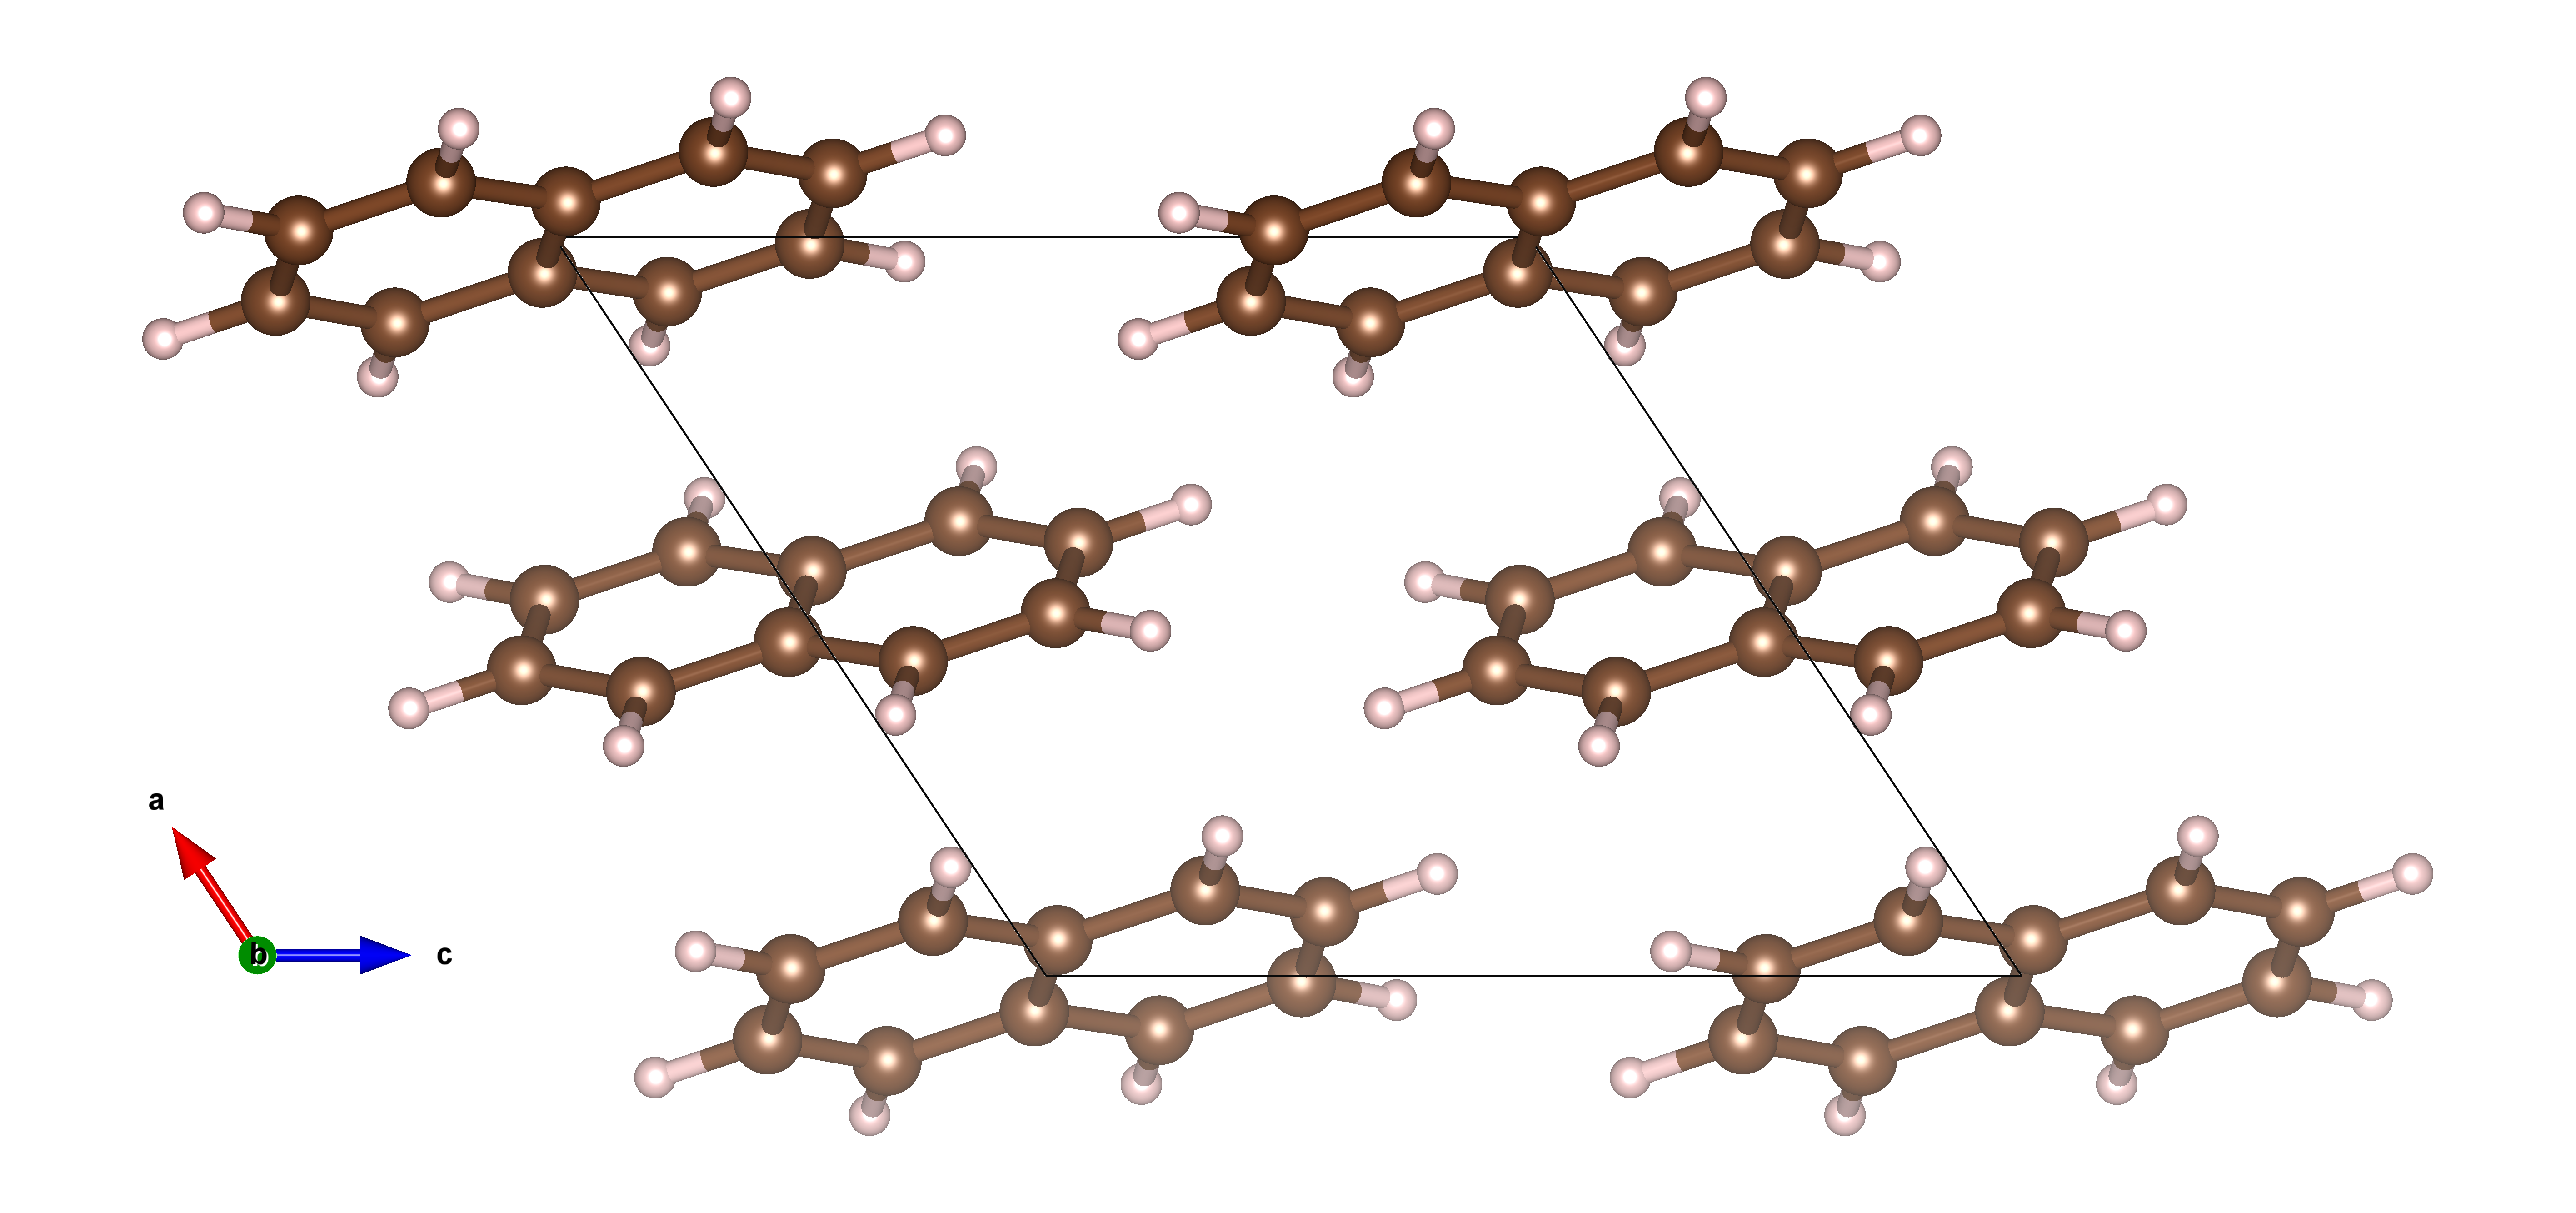
\includegraphics[scale=0.5]{image/Naphthalene-b}	& 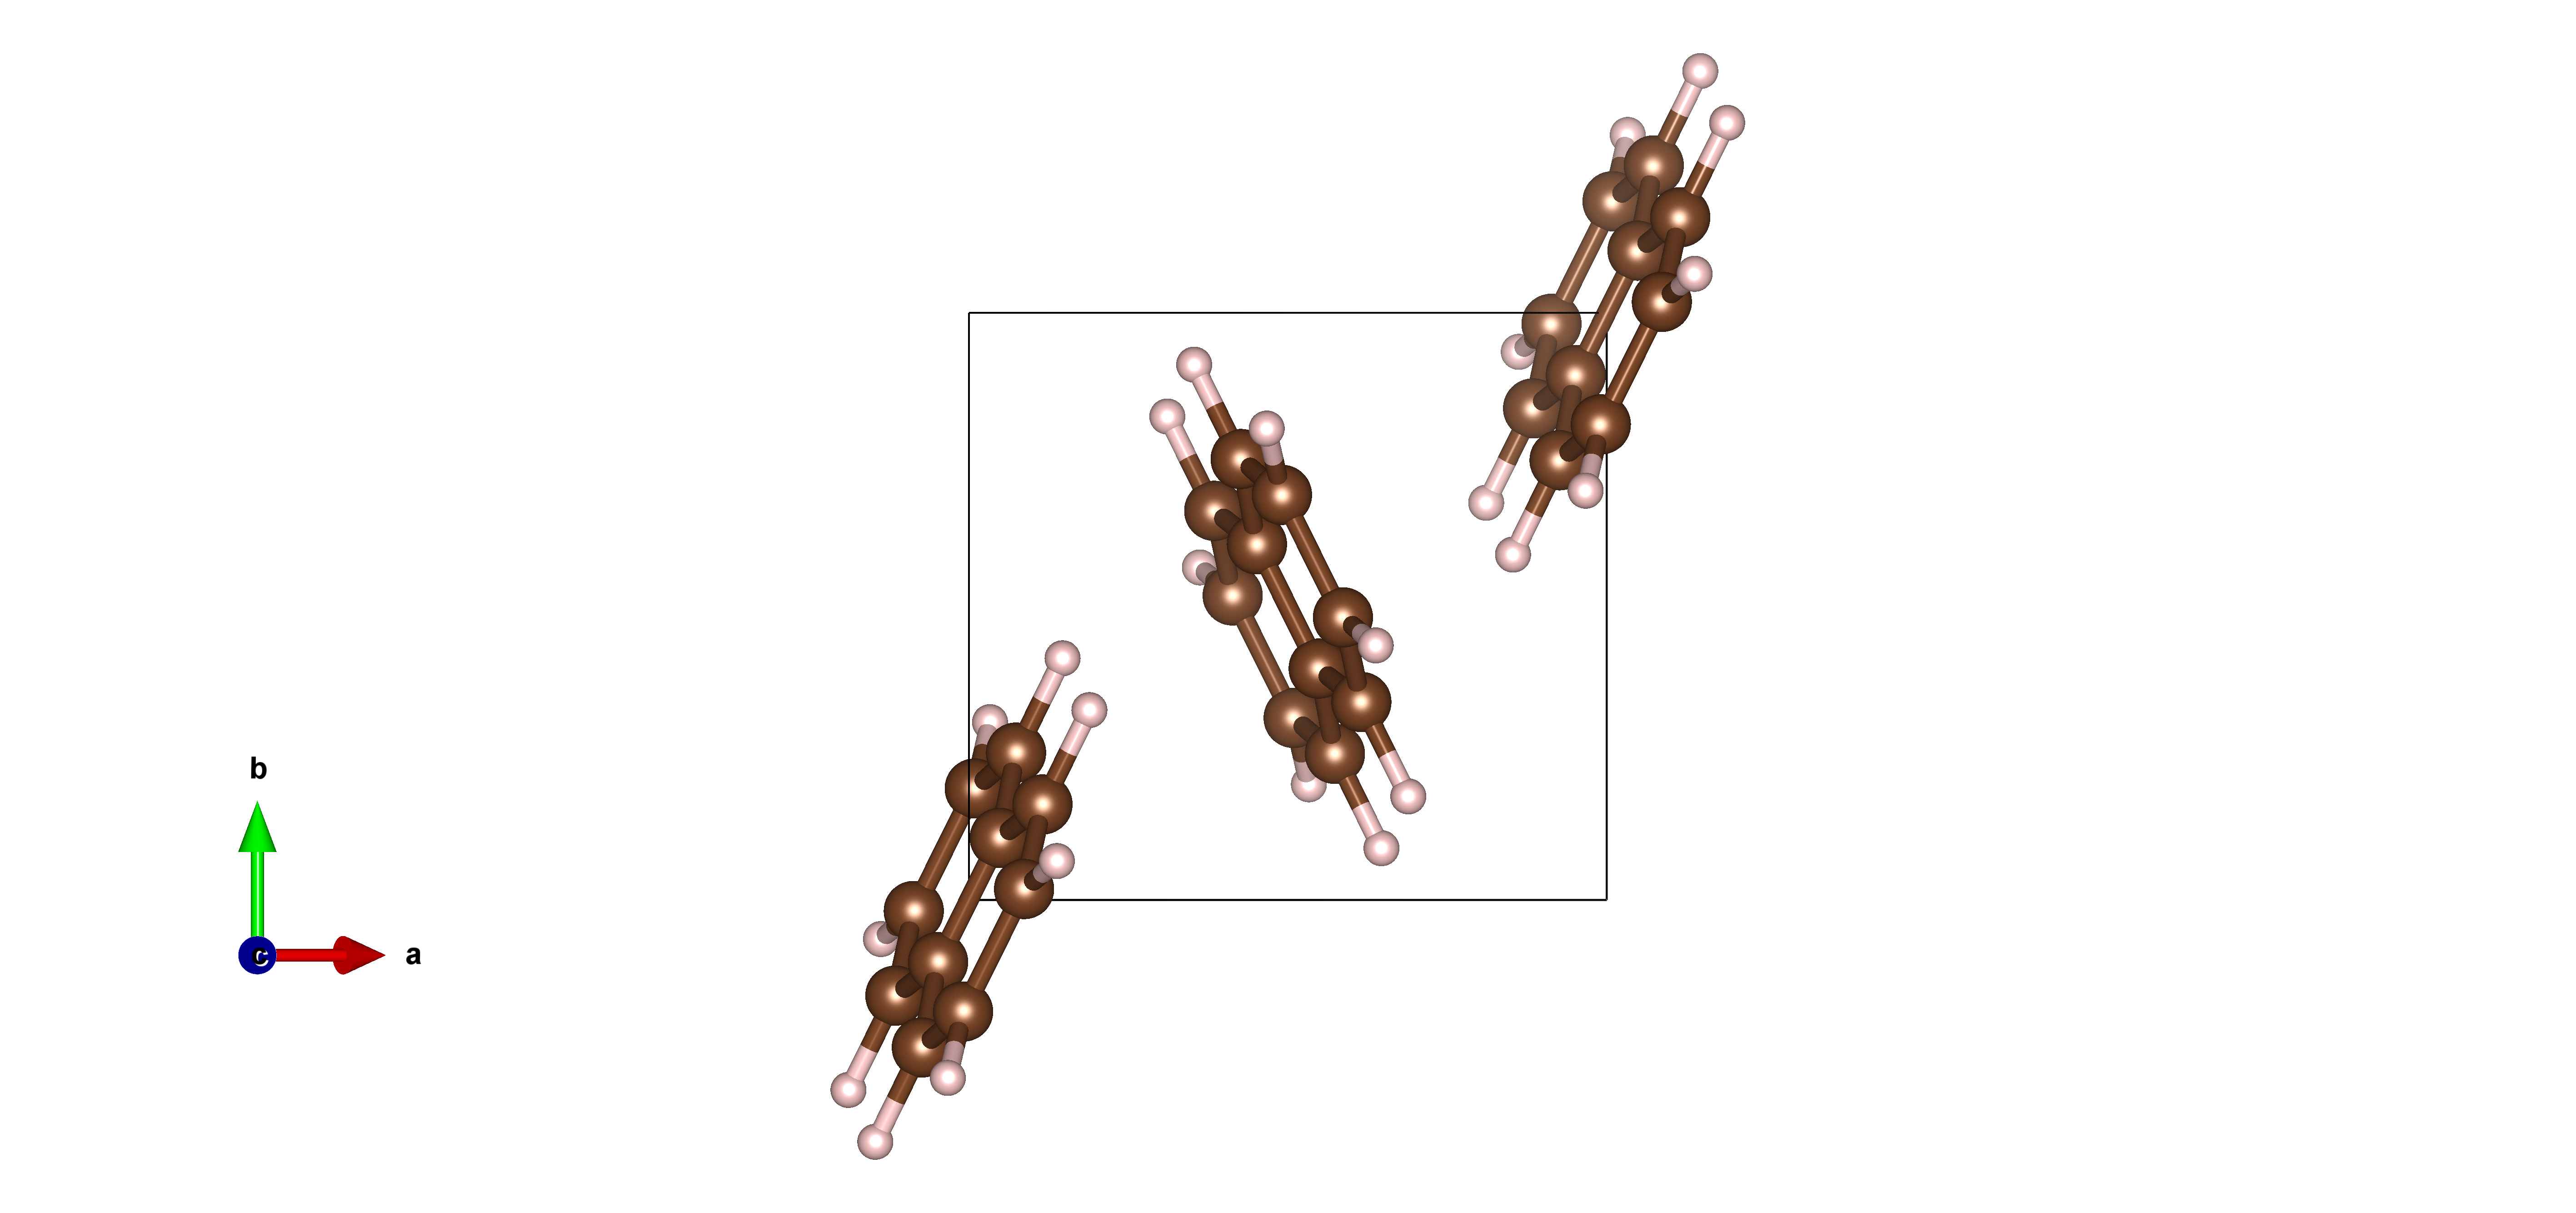
\includegraphics[scale=0.5]{image/Naphthalene-c} \\	
 			\end{tabular}}
 		\caption{The \textit{ac} and \textit{ab} planes of Naphthalene crystal} \label{fig-Naphsol}	
 		\end{center}
 	\end{figure}
 

 	
 	\begin{table}[H]
 		\caption{Lattice parameters of Naphthalene molecule calculated in VASP code} \label{table-Naphsol}
 		\begin{center}
 			\begin{threeparttable}
 			\begin{tabular}{c c c c c c c}
 				\toprule
 				& \textbf{D2} & \textbf{D3} & \textbf{TS} & \textbf{TS-SCS} & \textbf{PBE*} & \textbf{Exp} ref\cite{fabbiani2006exploration} \\
 				\midrule
 				\textbf{a} &7.71 (7.78) & 8.00 & 7.85 & 7.89 & 9.64 & 8.03\\
 				\textbf{b}& 5.84 (5.74) & 6.07 & 6.01 & 6.03 & 6.51 & 5.89 \\
 				\textbf{c}& 8.50 (8.57) & 8.68 & 8.63 & 8.65 & 9.14 & 8.57 \\
 				\textbf{$\beta$} & 125.18 (125.25) & 123.40 & 123.68 & 123.69 & 121.46 & 123.59\\
 				\textbf{Volume ($\AA^{3}$)} & 313.24 (312.75) & 351.97 & 338.45 & 342.52 & 488.96 & 337.65\\
 				\bottomrule
 			\end{tabular}
 			
 			\begin{tablenotes}
 				\item[*] without dispersion correction
 				\item[()] Parenthesis values were calculated with CRYSTAL program
 			\end{tablenotes}
 		\end{threeparttable}
 		\end{center}
 	\end{table}
 


\begin{figure}[H]
	\begin{center}
		\resizebox{20cm}{!}{
			\begin{tabular}{c c}
				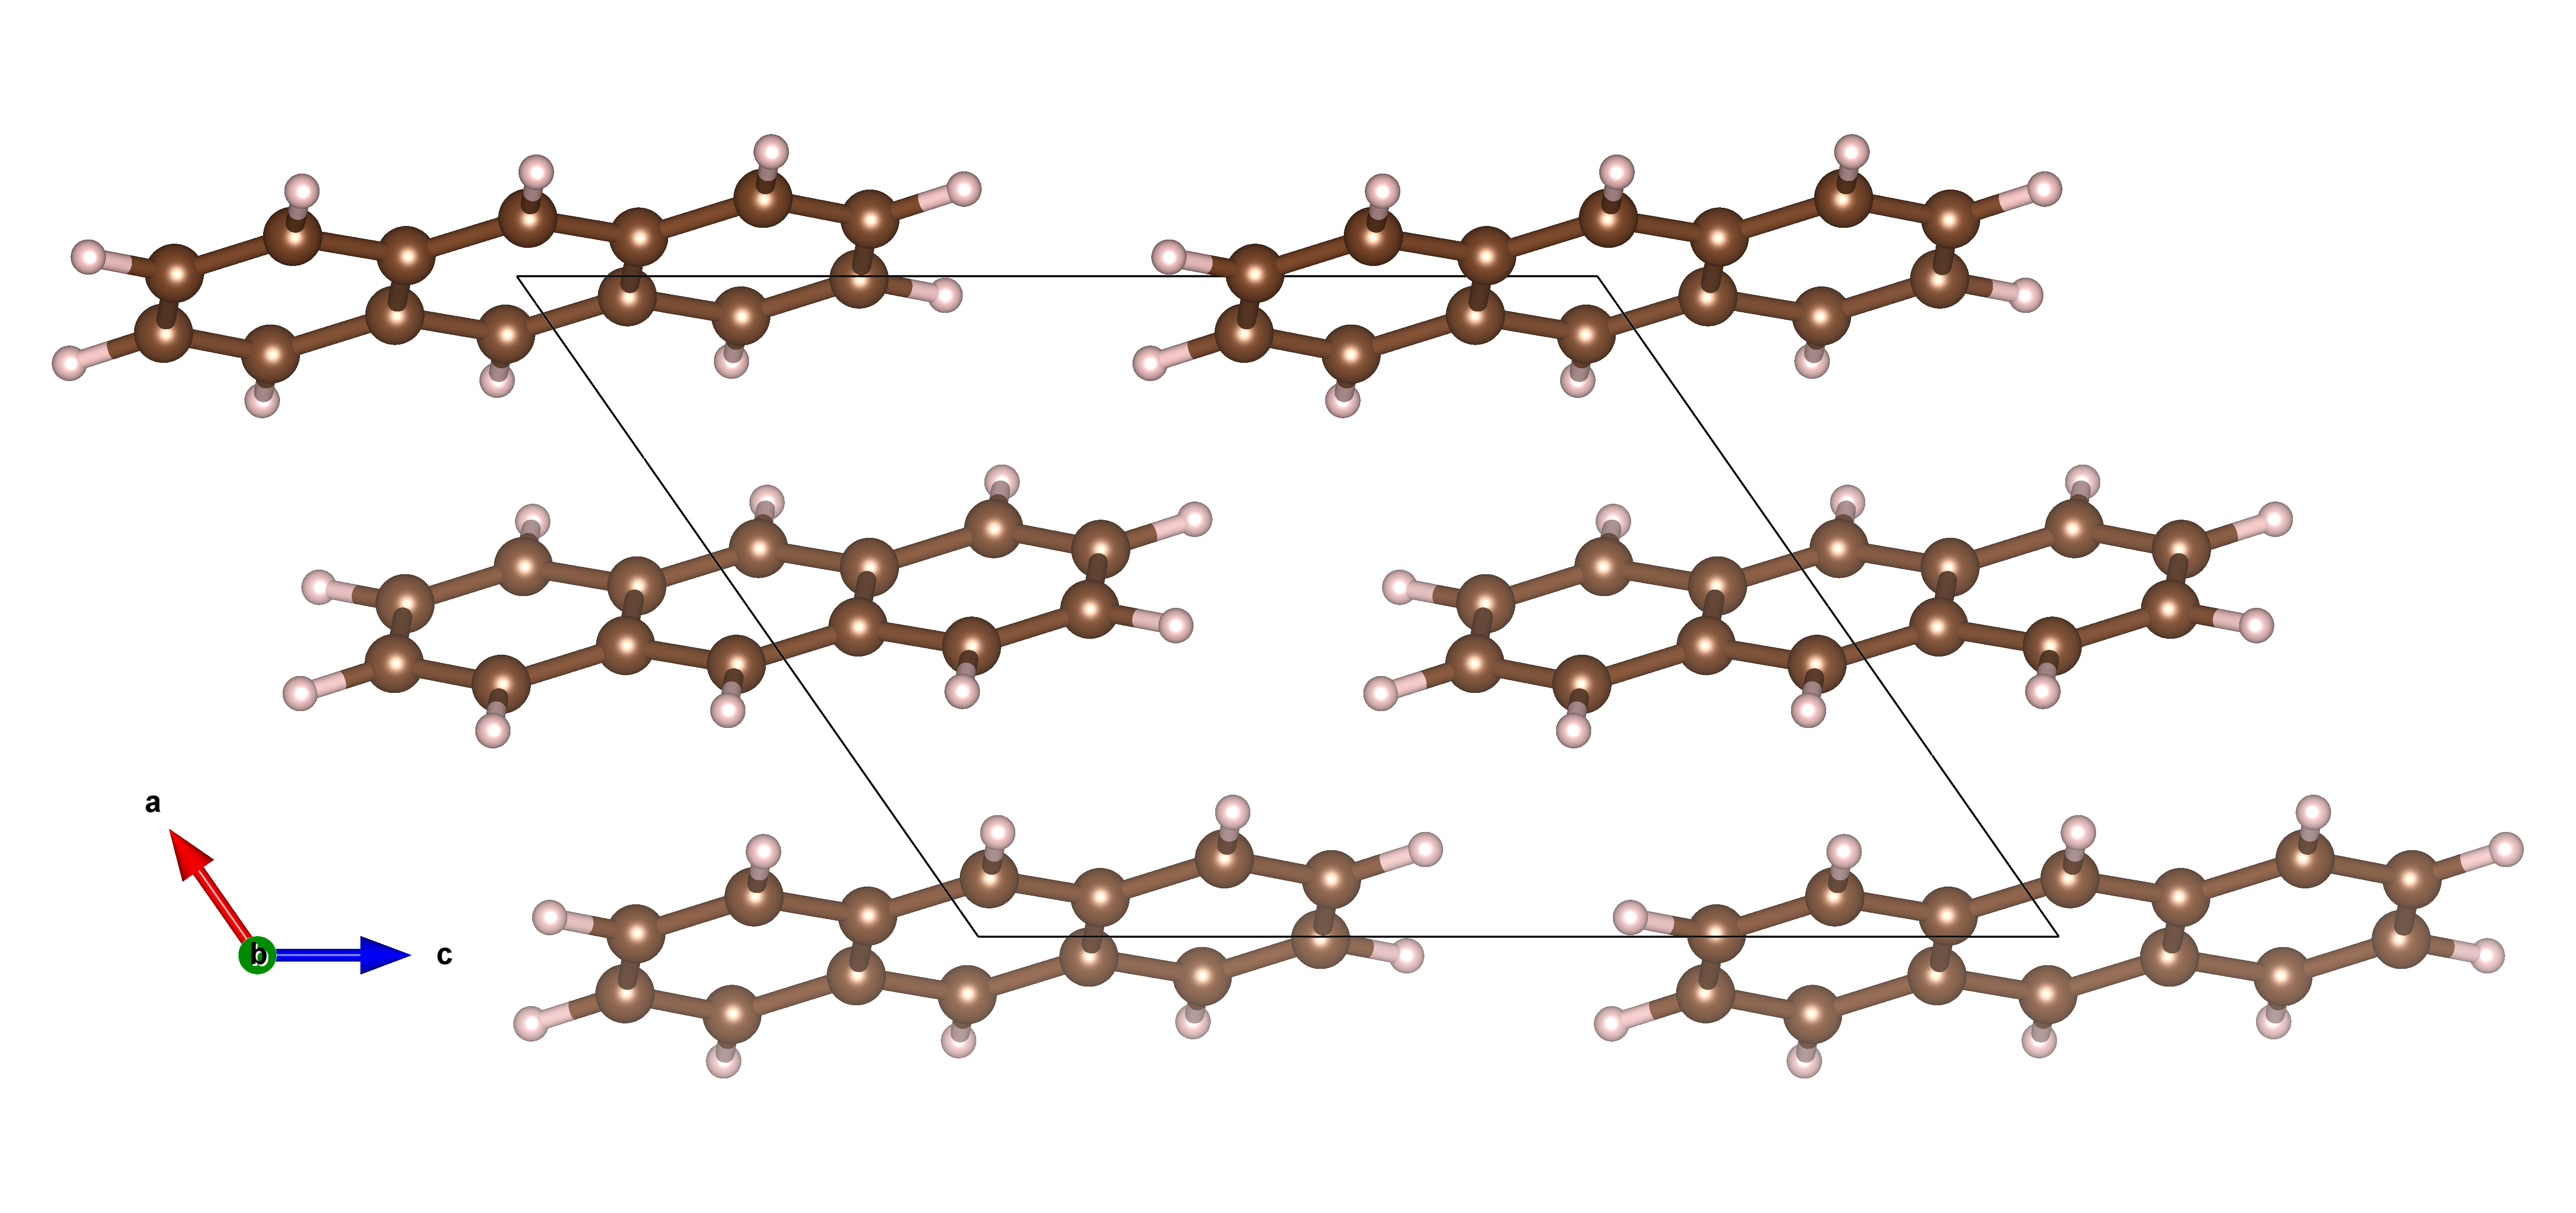
\includegraphics[scale=0.5]{image/Anthracene-b} & 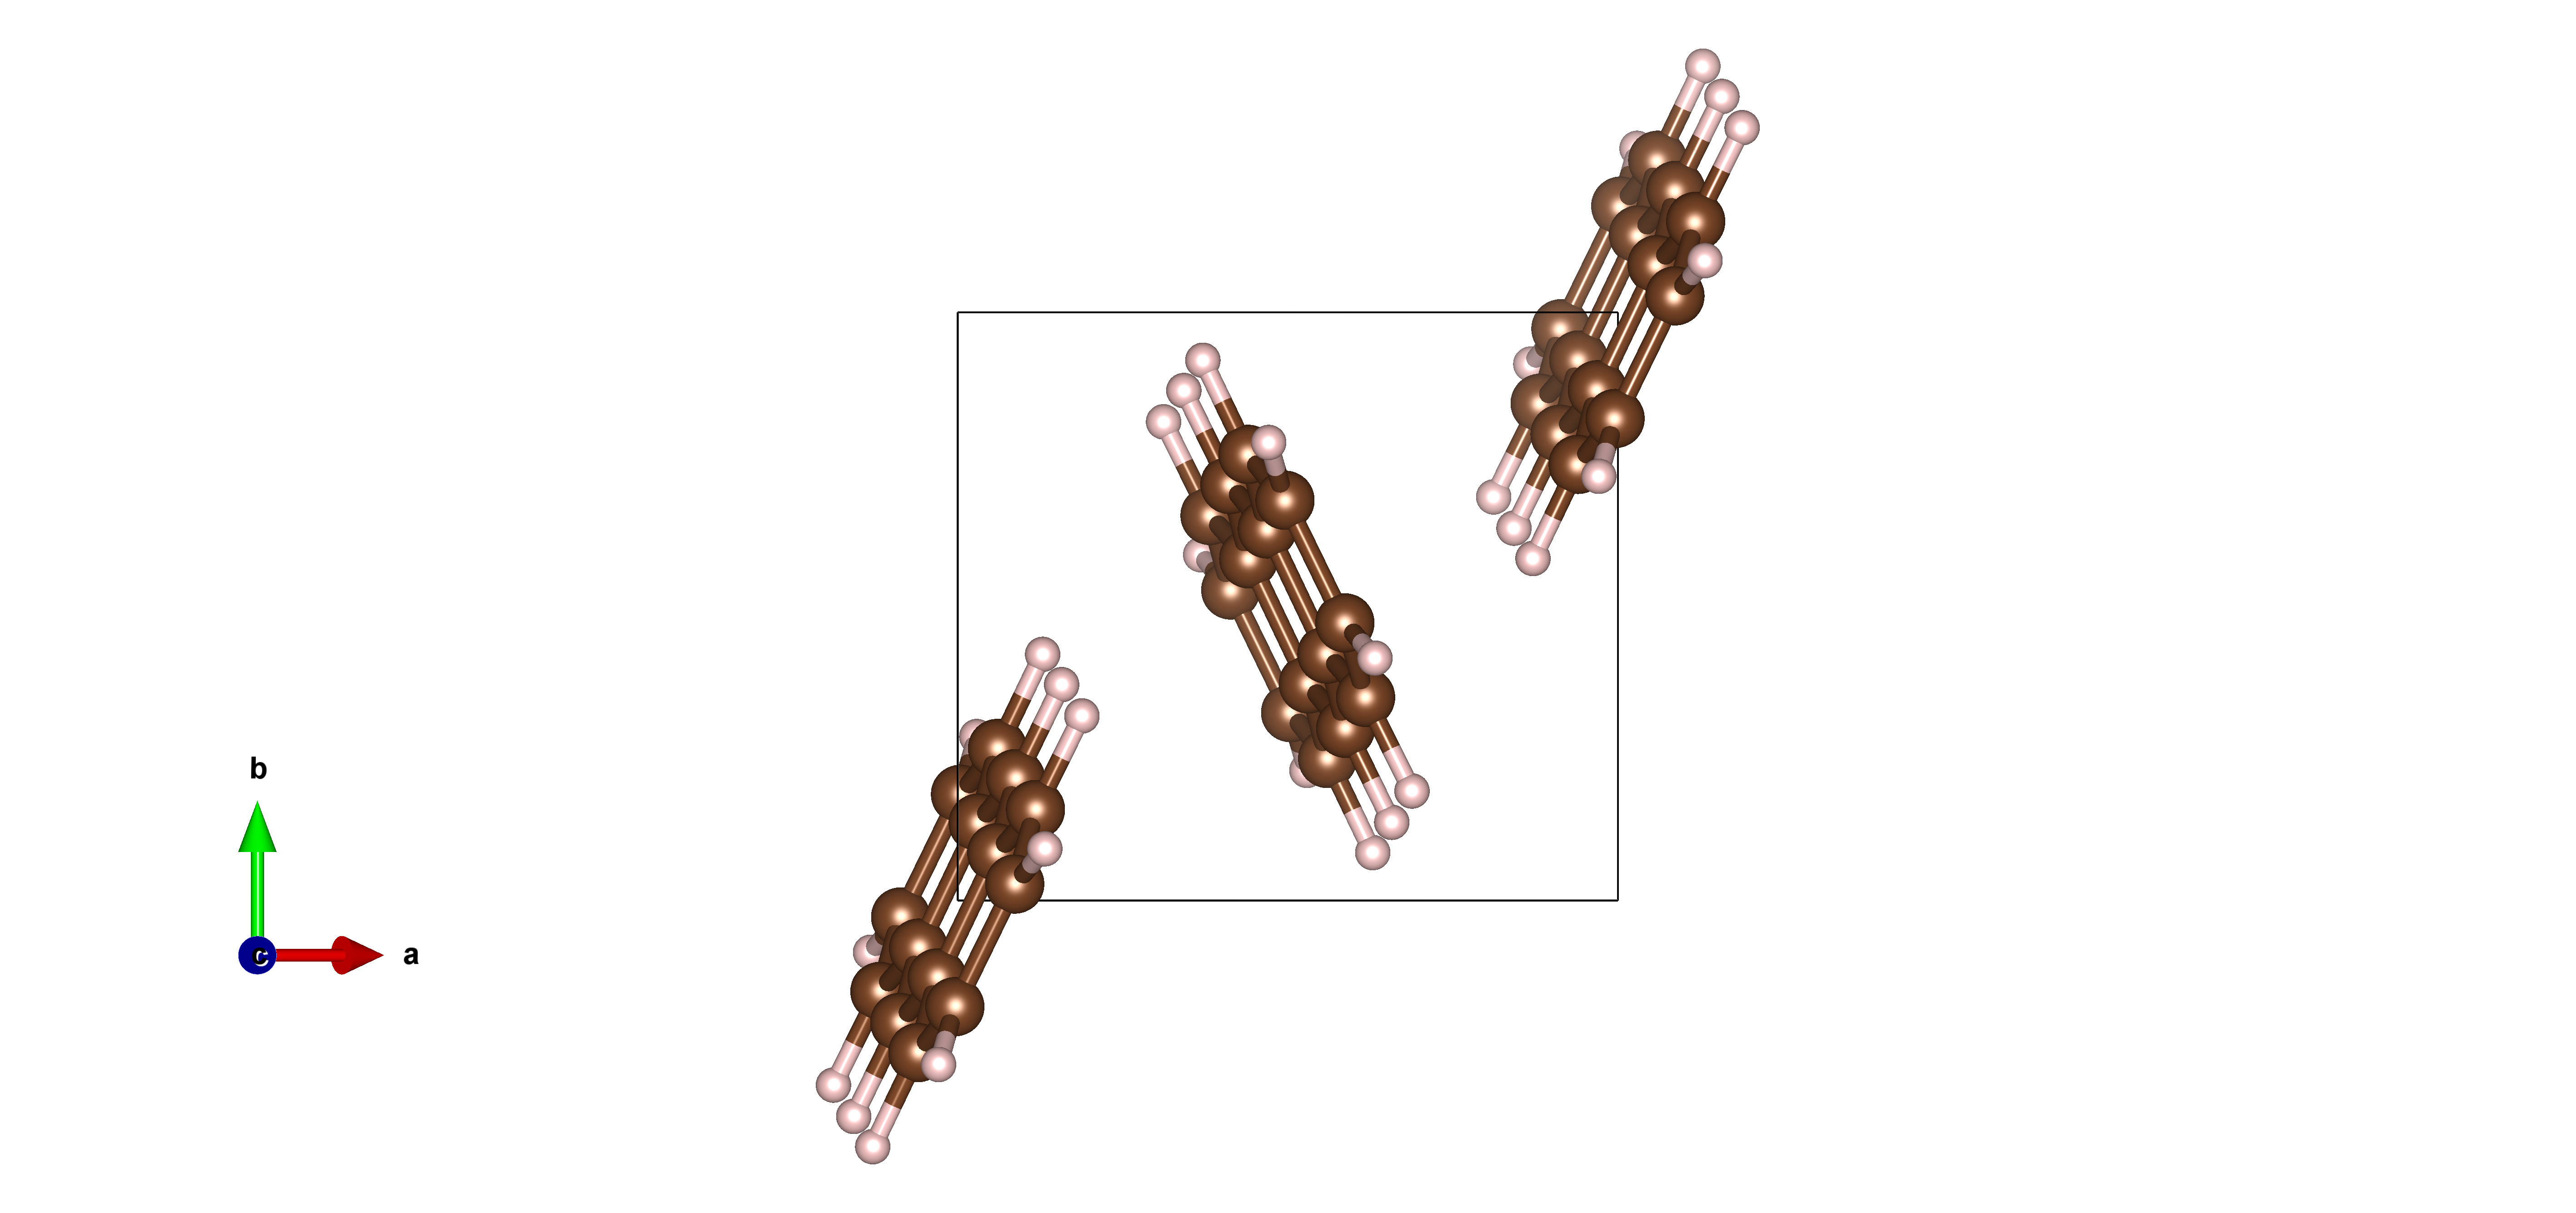
\includegraphics[scale=0.5]{image/Anthracene-c} \\	
			\end{tabular}}
			\caption{The \textit{ac} and \textit{ab} planes of Anthracene crystal}  \label{fig-Anthrasol}
		\end{center}
	\end{figure}



 
 	\begin{table}[htb]
 		\caption{Lattice parameters of Anthracene molecule calculated in VASP code} \label{table-Anthrasol}
 		\begin{center}
 			\begin{threeparttable}
 			\begin{tabular}{c c c c c c c}
 				\toprule
 				& \textbf{D2} & \textbf{D3} & \textbf{TS} & \textbf{TS-SCS} & \textbf{PBE*} & \textbf{Exp} ref\cite{brock1990temperature} \\
 				\midrule
 				\textbf{a} &8.04 (8.40) & 8.39 &8.23 & 8.26 & 9.97 &8.55 \\
 				\textbf{b}& 5.99 (5.67) & 6.12 & 6.03 & 6.07 & 6.54 & 6.02 \\
 				\textbf{c}& 11.14 (11.30) & 11.25 & 11.17 & 11.21 & 11.60 & 11.17 \\
 				\textbf{$\beta$} & 126.09 (128.26) & 124.95 & 125.46 & 125.42 & 121.61 & 124.60\\
 				\textbf{Volume ($\AA^{3}$)} & 433.85 (422.71) & 473.17 & 452.06 & 457.75 & 644.25 & 473.17\\
 				\bottomrule
 			\end{tabular}
 			
 			\begin{tablenotes}
 				\item[*] without dispersion correction
 				\item[()] Parenthesis values were calculated with CRYSTAL program
 			\end{tablenotes}
 		\end{threeparttable}
 		\end{center}
 	\end{table}
 
 \begin{figure}[H]
 	\begin{center}
 		\resizebox{20cm}{!}{
 			\begin{tabular}{c c}
 			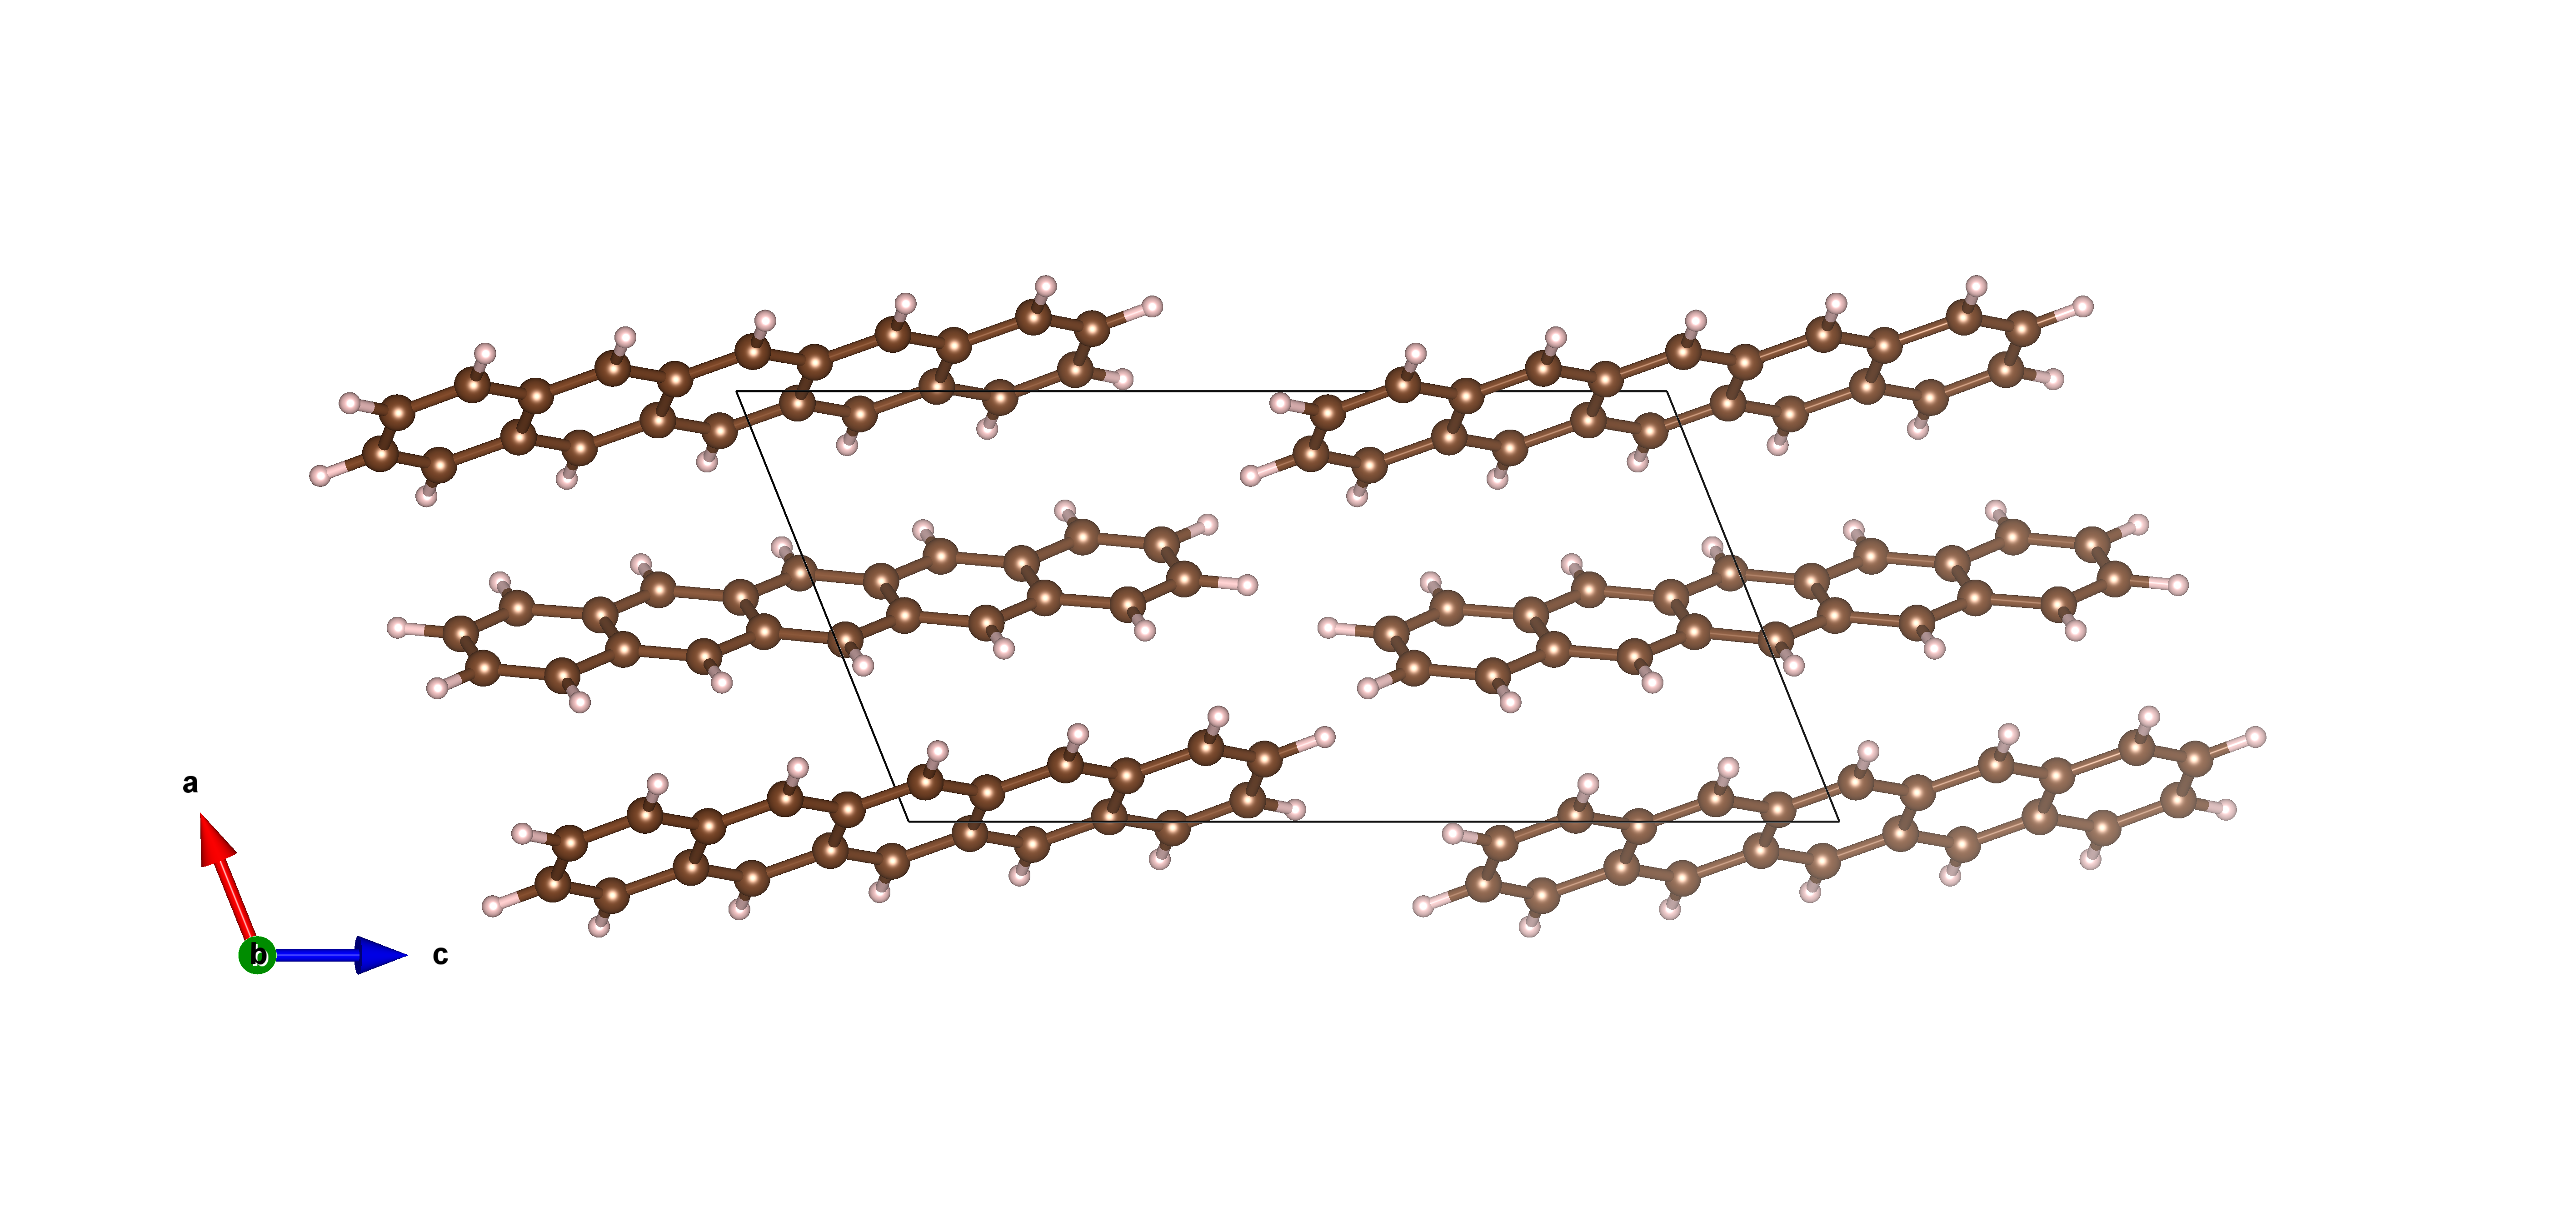
\includegraphics[scale=0.5]{image/PentaceneC-b} &  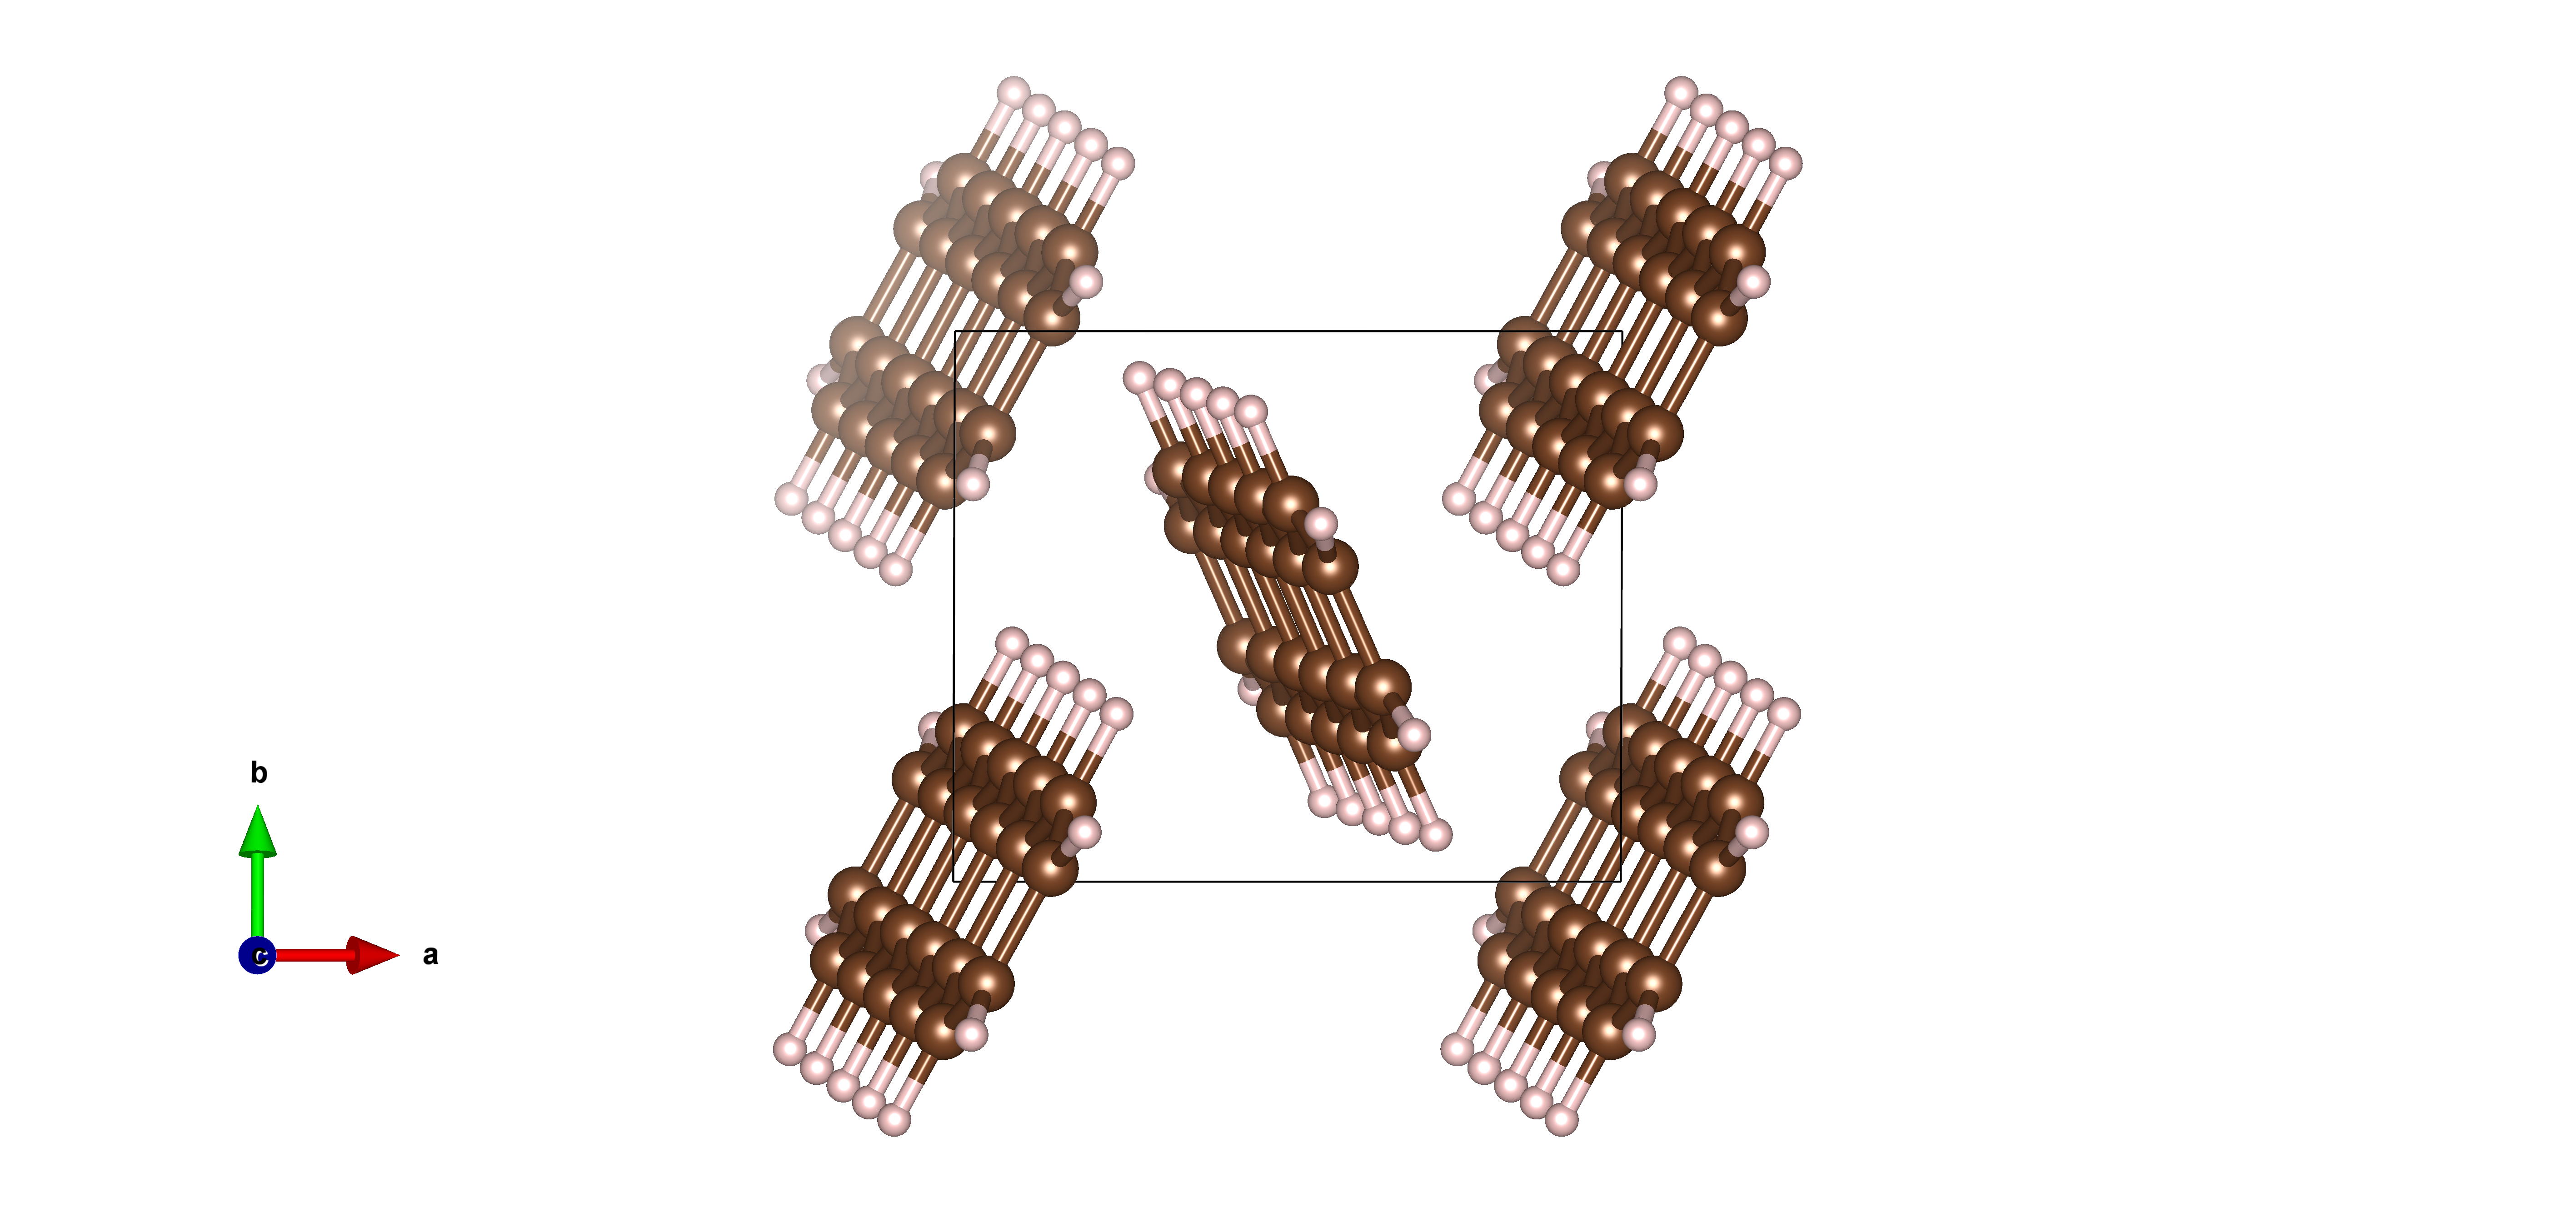
\includegraphics[scale=0.5]{image/PentaceneC-c}  \\
 			\end{tabular}}
 			\caption{The \textit{ac}, \textit{ab} planes of Pentacene polymorph C.}  \label{fig-Pentasol}	
 		\end{center}
 	\end{figure}
 
 
 
  \begin{figure}[H]
  	\begin{center}
  		\resizebox{20cm}{!}{
  			\begin{tabular}{c}
  			  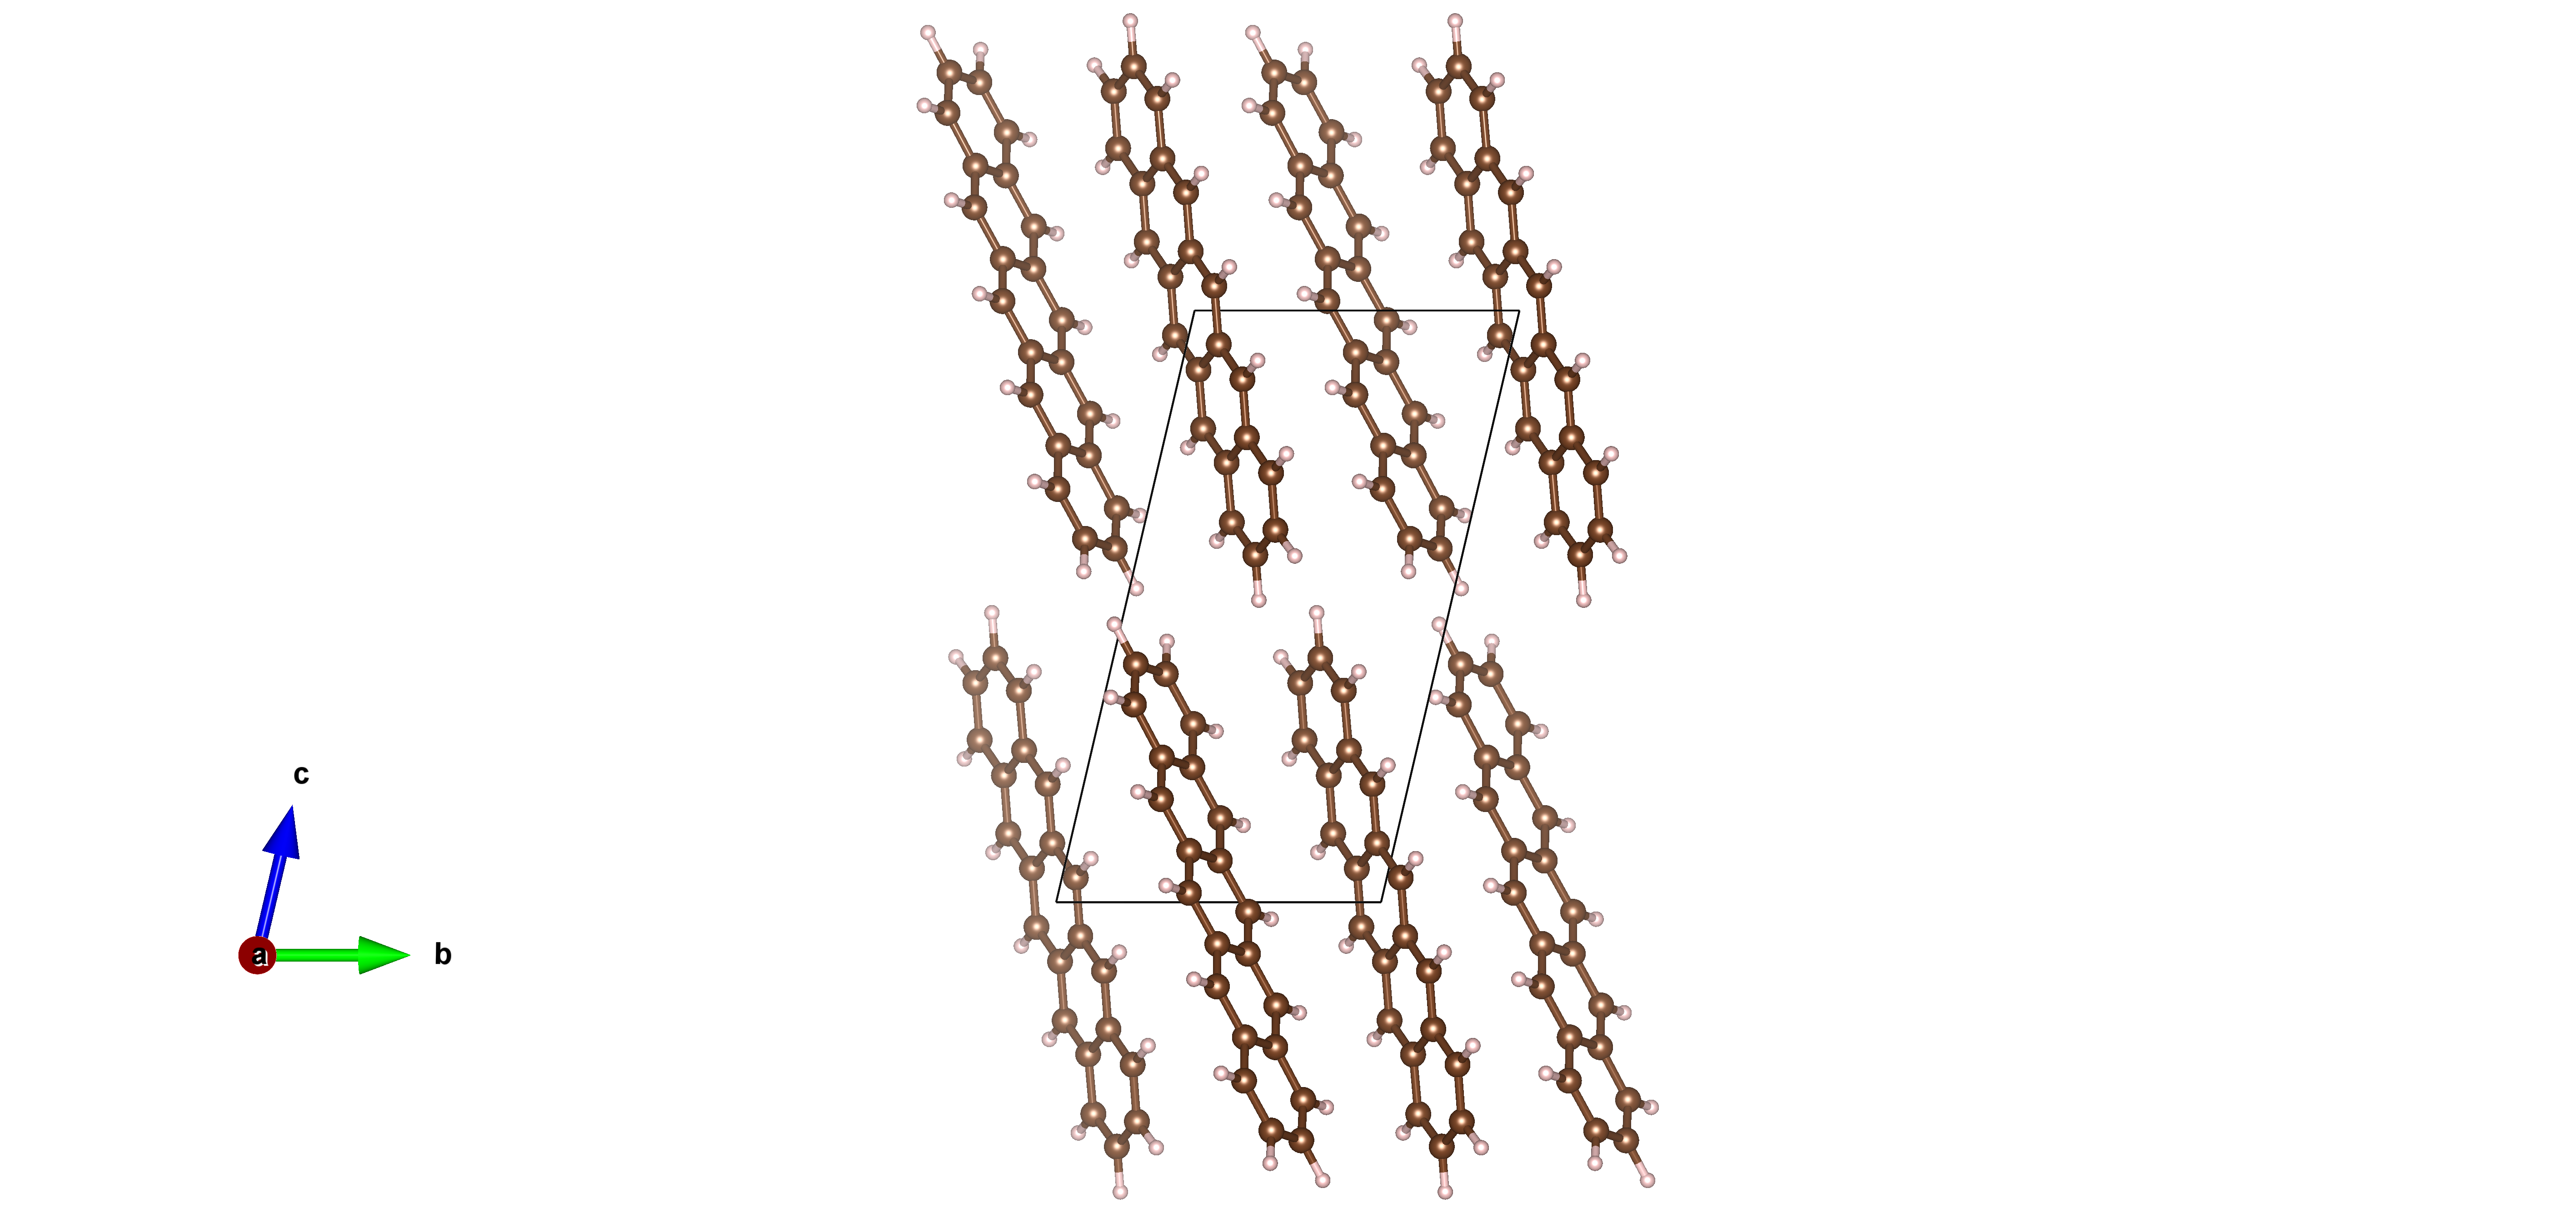
\includegraphics[scale=0.2]{image/PentaceneH-a}\\
  			\end{tabular}}
  			\caption{The \textit{bc} plane of Pentacene polymorph H at the bottom} 	
  		\end{center}
  	\end{figure}

 		
 	
 	\begin{table}[htb]
 		\caption{Lattice parameters of Pentacene molecule (Polymorphe H) calculated in VASP code} \label{table-penta}
 		\begin{center}
 			\begin{threeparttable}
 			\begin{tabular}{c c c c c c c}
 				\toprule
 				& \textbf{D2} & \textbf{D3} & \textbf{TS} & \textbf{TS-SCS} & \textbf{PBE*} & \textbf{Exp} ref\cite{mattheus2001polymorphism} \\
 				\midrule
 				\textbf{a} &6.16 (6.18) & 6.27 & 6.13 & 6.37 & 6.93 & 6.27\\
 				\textbf{b}& 7.25 (7.32) & 7.77 & 7.54 & 7.68 & 8.79 & 7.78 \\
 				\textbf{c}& 13.96 (13.98) & 14.48 & 14.33 & 14.46 & 15.36 & 14.53 \\
 				\textbf{$\alpha$} & 78.99 (78.92) & 76.72 & 77.89 & 77.62 & 72.10 &76.48\\
 				\textbf{$\beta$} & 88.69 (90.73) & 88.19 & 87.76 & 87.66 & 86.85 & 87.68\\
 				\textbf{$\gamma$} & 83.83(83.00) & 84.43 & 84.49 & 84.42 & 85.07 & 84.68\\
 				\textbf{Volume ($\AA^{3}$)} & 608.37 (615.63) & 683.04 & 644.52 & 687.62  & 886.39 & 685.15\\
 				\bottomrule
 			\end{tabular}
 			
 			\begin{tablenotes}
 				\item[*] without dispersion correction
 				\item[()] Parenthesis values were calculated with CRYSTAL program
 			\end{tablenotes}
 		\end{threeparttable}
 		\end{center}
 	\end{table}
 	
 	\begin{table}[H]
 		\caption{Lattice parameters of pentacene molecule (polymorphe C) calculated in VASP code} \label{table-pentaC}
 		\begin{center}
 			\begin{threeparttable}
 			\begin{tabular}{c c c c c c c}
 				\toprule
 				& \textbf{D2} & \textbf{D3} & \textbf{TS} & \textbf{TS-SCS} & \textbf{PBE*} & \textbf{Exp} ref\cite{campbell1961crystal} \\
 				\midrule
 				\textbf{a} &7.40 (7.02) & 7.81 & 7.67 & 7.61 & 9.03 & 7.90\\
 				\textbf{b}& 5.98 (5.70) & 6.09 & 6.02 & 6.09 & 6.54 & 6.06 \\
 				\textbf{c}& 15.70 (15.68) & 15.97 & 15.82 & 15.92 & 16.23 & 16.01 \\
 				\textbf{$\alpha$} & 102.67 (89.98) & 101.97 & 102.08 & 101.40 & 101.91 & 101.90\\
 				\textbf{$\beta$} & 113.48 (97.19) & 112.31 & 112.73 & 112.57 & 110.91 & 112.60\\
 				\textbf{$\gamma$} &84.98 (90.00) & 85.33 & 85.53 & 85.63 & 86.42 & 85.80\\
 				\textbf{Volume ($\AA^{3}$)} & 622.05 (622.95) & 686.75 & 659.16 & 668.18  & 878.28 & 692.38\\
 				\bottomrule
 			\end{tabular}
 			
 				\begin{tablenotes}
 					\item[*] without dispersion correction
 					\item[()] Parenthesis values were calculated with CRYSTAL program
 				\end{tablenotes}
 			\end{threeparttable}
 		\end{center}
 	\end{table}


The results associated to the acene family, i.e., benzene, naphthalene, anthracene and pentacene, are reported in Tables \ref{table-benzsol}- 7 hereafter. The calculation conditions in this piece of modelling are identical to those used just before for the tetracene molecule. The main conclusions arising from the study of these systems are in agreement with those obtained for the tetracene system. Indeed, for these systems, the structural parameters and unit cell volumes are better described by the PBE-D3 level of theory if a comparison is made with the other methods used in this work (except for the two anthracene and benzene systems where the TS and the TSC data are in relative better agreement in comparison to the experimental data \cite{buvcko2013tkatchenko}). The agreement between our theoretical and experimental data meets the requirements to the frequency calculation of the crystalline network. Moreover, the inclusion of the dispersive terms (like D3 or the modified D2:TS) must be introduce onto the frequency calculation because of the well-known dispersive character of the intermolecular modes to describe. The vibrational results calculated for these systems are reported in Table \ref{table-freqBen}- 11 in which the frequency values can also be found for each acene family-member monomer and dimer. According to the conclusions drawn for the tetracene system case, one can find for these systems at least an active signature associated to a network vibrational mode around 100 cm$^{-1}$ (88 and 106 cm$^{-1}$ for naphthalene, 98 cm$^{-1}$ for anthracene, and 102 cm$^{-1}$ for pentacene). One should note that the benzene molecule (also in the acene family) in its T-Shape conformation needs a specific analysis. As a matter of fact, for this conformation, the intermolecular interactions of the crystal network do not correspond any longer to the simple $\pi$-$\pi$ interactions (as it is the case of the other systems herein studied) but to interactions of the type $\pi$-H, as demonstrated by Katrusiak et al \cite{katrusiak2010association}. Yet, although the interactions are of different nature, our calculations show that the main active vibrational signature of the crystalline network remains localised in the 100-130 cm$^{-1}$ region. Moreover, in the following paragraphs, it will be shown that the spectral position remains unchanged for different systems only for this (these) specific mode(s). For all the other modes, depending on the symmetry of the system and on the strength of the long-range interactions between neighbour molecules, the spectral signatures can vary in position and in intensity. This observation only constitutes the major information to be extracted from our calculations given the aim of this work.	
 	
 				
 				\begin{table}[H]
 					\caption{ Calculated vibrational frequencies (cm$^{-1}$) of the monomer, dimer and solid-state (PBE Benzene system).}  \label{table-freqBen}
 					\begin{center}
 						\begin{threeparttable}
 						\begin{tabular}{c c c c c}
 							\toprule
 							\multicolumn{2}{p{4.5cm}}{\centering \textbf{Monomer}} & \textbf{Dimer} & \multicolumn{1}{p{4cm}}{\centering \textbf{Experimental}} & \textbf{VASP/CRYSTAL}\\
 							Assignment & $\nu$(cm$^{-1}$) & $\nu$(cm$^{-1}$) & $\nu$(cm$^{-1}$) & $\omega$(cm$^{-1}$) \\
 							& Int(km/mol) & Int(km/mol) & & Int(km/mol) \\
 							\midrule
 							&  &  \textit{7 (0.04)}& & \\
 							&  & \textit{12 (<0.01)} &  & \\
 							&  & \textit{48 (<0.01)}&  & \\
 							& & \textit{56 (0.07)} &  & \\
 							&  & \textit{63 (0.08)}&  & \textit{63 (0.69)} \\
 							&  & \textit{75 (0.03)} &  & \textit{71 (0.05)} \\
 							&   &  &    &  \textit{101 (0.69)}\\
 							&   & &  & \textit{119 (4.24)}\\
 							&   &   &   &  \textit{126 (1.11)}\\
 							&   &   &   & \textit{128 (4.83)}\\
 							\multirow{2}{2cm}{\centering $\nu_{1}$}& \multirow{2}{2cm}{\centering 426 (0)} & 424 (0.003) &   & 410 (0.05)\\
 							&   &   425 (0.003) &  & 419 (0.79)\\ 
 							\bottomrule	    
 						\end{tabular}
 						
 						\begin{tablenotes}
 							\item[] Italic: Intermolecular modes
 						\end{tablenotes}
 					\end{threeparttable}
 					\end{center}
 				\end{table}	
 				
 	
 	
 	\begin{table}[H]
 		\caption{ Calculated vibrational frequencies (cm$^{-1}$) of the monomer, dimer and solid-state (PBE Naphthalene system).} \label{table-freqNaph}
 		\begin{center}
 			\begin{threeparttable}
 				\begin{tabular}{c c c c c}
 					\toprule
 					\multicolumn{2}{p{4.5cm}}{\centering \textbf{Monomer}} & \textbf{Dimer} & \multicolumn{1}{p{4cm}}{\centering \textbf{Experimental} \\ ref \cite{krainov1964vibrational}} & \textbf{VASP/CRYSTAL}\\
 					Assignment & $\nu$(cm$^{-1}$) & $\nu$(cm$^{-1}$) & $\nu$(cm$^{-1}$) & $\omega$(cm$^{-1}$) \\
 					& Int(km/mol) & Int(km/mol) & & Int(km/mol) \\
 					\midrule
 					&  & \textit{33 (0.04)} & & \\
 					&  & \textit{36 (0)} &  & \\
 					&  & \textit{55 (0)} &  & \\
 					&  & \textit{75 (0.21)} &  & \textit{88 (1.74)}\\
 					&  & \textit{88 (0.08)} &  & \textit{106 (1.78)}\\
 					&  & \textit{101 (0)} &  & \\
 					\\
 					\multirow{2}{2cm}{\centering $\nu_{1}$} & \multirow{2}{2cm}{\centering 177 (3.2)}& 181 (3.8) & \multirow{2}{2cm}{\centering 176} & \multirow{2}{2cm}{\centering 174 (2.60)}\\
 					&   &   188 (0) &  & \\
 					\multirow{3}{2cm}{\centering $\nu_{2}$} & \multirow{3}{2cm}{\centering 191 (0)}& 201 (1.2) & \multirow{3}{2cm}{\centering 195} & 190 (0.04)\\
 					&   &   201 (0) &  & 208 (0.03)\\
 					&   &    &   & 210 (1.26)\\
 					\multirow{2}{2cm}{\centering $\nu_{3}$} & \multirow{2}{2cm}{\centering 379 (1.5)}& 372 (2.2) & \multirow{2}{2cm}{\centering 359} & 362 (0.35)\\
 					&   &   372 (0) &  & 364 (1.54)\\
 					\multirow{2}{2cm}{\centering $\nu_{4}$} & \multirow{2}{2cm}{\centering 403 (0)}& \multirow{2}{2cm}{\centering 396 (0.02)} &  & 386 (0)\\
 					&   &   &  & 391 (0)\\
 					\bottomrule	    
 				\end{tabular}
 				
 				\begin{tablenotes}
 					\item[] Italic : Intermolecular modes
 				\end{tablenotes}
 			\end{threeparttable}
 		\end{center}
 	\end{table}	
 	
 	
 	\begin{spacing}{1.1}
 		\begin{table}[H]
 			\caption{ Calculated vibrational frequencies (cm$^{-1}$) of the monomer, dimer and solid-state (PBE Anthracene system).} \label{table-freqAnthra}
 			\begin{center}
 				\begin{threeparttable}
 				\begin{tabular}{c c c c c}
 					\toprule
 					\multicolumn{2}{p{4.5cm}}{\centering \textbf{Monomer}} & \textbf{Dimer} & \multicolumn{1}{p{4cm}}{\centering \textbf{Experimental} \\ ref \cite{kalescky2013description}/ ref \cite{bree1968infrared}} & \textbf{VASP/CRYSTAL}\\
 					Assignment & $\nu$(cm$^{-1}$) & $\nu$(cm$^{-1}$) & $\nu$(cm$^{-1}$) & $\omega$(cm$^{-1}$) \\
 					& Int(km/mol) & Int(km/mol) & & Int(km/mol) \\
 					\midrule
 					&  &  \textit{22 (0.004)} & & \\
 					&  & \textit{34 (0)} &  & \\
 					& & \textit{57 (0)} &63 (m) & \\
 					&  & \textit{75 (0.05)} & 72 (w)& \\
 					&  & \textit{87 (0.8)} & & \textit{98(1.37)}\\
 					\\
 					\multirow{2}{2cm}{\centering $\nu_{1}$} & \multirow{2}{2cm}{\centering 93 (1.5)} & 111 (0.8)& \multirow{1}{2cm}{\centering 106/104(m)} & 101 (4.03)\\
 					& & 112 (1.2) & 110 (s) & 119 (0.05)\\
 					\multirow{2}{2cm}{\centering $\nu_{2}$} & \multirow{2}{2cm}{\centering 124 (0)}& 148 (0.6) & \multirow{1}{2cm}{\centering 137/126(s)} & 153 (1.77)\\
 					&  & 149 (0.02) &166 (s) & 155 (0.07)\\
 					\multirow{2}{2cm}{\centering $\nu_{4}$}& \multirow{2}{2cm}{\centering 243 (1.4)} & 244 (2.1) & \multirow{2}{2cm}{\centering 234 \\ 235 (s)} & 239 (1.25)\\
 					& & 244 (0) &  & 239 (0.33)\\ 
 					\multirow{2}{2cm}{\centering $\nu_{5}$}& \multirow{2}{2cm}{\centering 276 (1.1)} & 250 (0) & \multirow{2}{2cm}{\centering 244}& 236 (0)\\
 					&  & 253 (0.2) &  & 237 (0)\\
 					&   & 285 (0.02) & \multirow{2}{2cm}{\centering 287}& 278 (0)\\
 					& & 286 (0.08) &  & 281 (0)\\
 					\multirow{2}{2cm}{\centering $\nu_{6}$} & \multirow{2}{2cm}{\centering 394 (0.05)}& 396 (0.2) & \multirow{1}{2cm}{\centering 380/361(vw)} & 375 (0.23)\\
 					& & 396 (0.04) & 380 (w) & 379 (0.36)\\
 					\multirow{2}{2cm}{\centering $\nu_{7}$} &\multirow{2}{2cm}{\centering 407 (0)} & 407 (0) & \multirow{2}{2cm}{\centering 397} & 389 (0)\\
 					& & 407 (0.04) & & 391 (0)\\
 					\bottomrule	    
 				\end{tabular}
 				
 				\begin{tablenotes}
 					\item[] Italic: Intermolecular modes 
 				\end{tablenotes}
 			\end{threeparttable}
 			\end{center}
 		\end{table}
 	\end{spacing}
 		
 		
 			\begin{table}[H]
 				\caption{ Calculated vibrational frequencies (cm$^{-1}$) of the monomer, dimer and solid-state (PBE Pentacene system).} \label{table-freqPenta}
 				\begin{center}
 					\begin{threeparttable}
 					\begin{tabular}{c c c c c}
 						\toprule
 						\multicolumn{2}{p{5cm}}{\centering \textbf{Monomer}} & \textbf{Dimer} & \multicolumn{1}{p{4cm}}{\centering \textbf{Experimental} \\ \textbf{(P.A.) ref \cite{spillebout2014discerning}}} & \textbf{VASP/CRYSTAL}\\
 						Assignment & $\nu$(cm$^{-1}$) & $\nu$(cm$^{-1}$) & $\nu$(cm$^{-1}$) & $\omega$(cm$^{-1}$) \\
 						& Int(km/mol) & Int(km/mol) & & Int(relative) \\
 						\midrule
 						& & \textit{19 (<0.01)} & & \\
 						& & \textit{27 (0.0)} & & \\
 						&  38 (0.5) & 42 (0.4) &  & 58 (0.46) \\
 						& & \textit{57 (0.0)} & & \\
 						& & \textit{72 (0.9)} & & \\
 						& & \textit{74 (0.07)} & & \\
 						&  & 84 (0) & & \\
						& & \textit{95 (0.0)} & & \\
 						\\
 						\multirow{2}{2cm}{\centering $\nu_{3}$} & \multirow{2}{2cm}{\centering 97(0.003)} & 101 (0.002) & \multirow{2}{2cm}{\centering 102 (m)}  & \multirow{2}{2cm}{\centering \textit{102 (5.17)}}\\
 						& & 108 (0.2) & & \\
 						\multirow{2}{2cm}{\centering $\nu_{4}$}& \multirow{2}{2cm}{\centering 122 (1.0)} &\multirow{2}{2cm}{\centering 122 (1.5)} &\multirow{2}{2cm}{\centering 122 (m)} &117 (0.99)\\
 						&  &   &   &  127 (0.21)\\
 						&   &  125 (0.0) &   &  \multirow{2}{2cm}{\centering 134 (6.1)}\\
 						&  &  130 (0.08) &  &  \\
 						\multirow{2}{2cm}{\centering $\nu_{1} + \nu_{3}$} &\multirow{2}{2cm}{\centering 144 (0.04)} &  & \multirow{2}{2cm}{\centering 141 (m)} & 140 (0.68)\\
 						&  &   &   &  148 (1.58)\\ 
 						\multirow{2}{2cm}{\centering $\nu_{2}+ \nu_{3}$} & \multirow{2}{2cm}{\centering 164(<0.01)} & 168 (0.2) & \multirow{2}{2cm}{\centering 165 (vw)} &  \\
 						& & 168 (0.05) & & \\
 						&  &   & 188 (w) & 180 (2.54)\\
 						$\nu_{6}$ & 194 (1.4) & 204 (2.2) & 198 (m) & 204 (2.36) \\
 						$\nu_{3}+\nu_{4}$ & 224 (0.0) & \multirow{2}{2cm}{\centering 210(0.002)} & \multirow{2}{2cm}{\centering 223 (vw)} & \\
 						$\nu_{2}+ \nu_{5}$ & 222 (0.002) & & & \\
 						$\nu_{1}+ 2\nu_{3}$& 251 (0.0) & 247 (0.05) & \multirow{2}{2cm}{\centering 257 (w)} & \multirow{2}{2cm}{\centering 254 (0.29)}\\
 						$\nu_{9}$ & 265 (0.03) & 255 (0.02) &  & \\
 						$2\nu_{1}+ \nu_{6}$ & 274 (<0.01) &  & 272 (vw) & 272 (0.45)\\
 						$\nu_{3}+ \nu_{6}$& 291 (<0.01) & 302 (0.005) & \multirow{2}{2cm}{\centering 296 (w)} & \\
 						$\nu_{1}+ \nu_{9}$ & 292 (<0.01) & 303 (0.07)&  & \\	
 						$\nu_{2}+ \nu_{7}$ & 316 (<0.01) & & 317 (w)& \\
 						$\nu_{3}+ \nu_{8}$ & 346 (0.03) &  &  344 (vw) & \\
 						\multirow{2}{2cm}{\centering $\nu_{12}$} & \multirow{2}{2cm}{\centering 374 (0.1)} &  & \multirow{2}{2cm}{\centering 357 (w)} &352 (1.12)\\
 						&  &   &   & 355 (0.27)\\
 						\multirow{2}{2cm}{\centering $\nu_{13}$} & \multirow{2}{2cm}{\centering 374 (0.03)} &  & \multirow{2}{2cm}{\centering 381 (m)} & 382 (0.01)\\
 						&   &    &   & 386 (0.34)\\
 						\bottomrule	    
 					\end{tabular}
 					
 					\begin{tablenotes}
 						\item[] Italic: Intermolecular modes
 					\end{tablenotes}
 				\end{threeparttable}
 				\end{center}
 			\end{table}





%-------------------------------------------------------------------------------------------------------------------------
%-------------------------------------------------------------------------------------------------------------------------
%-------------------------------------------------------------------------------------------------------------------------
\section{Impact of both the chain-length and "widths" parameters on the vibrational signature of the crystalline network.}
%-------------------------------------------------------------------------------------------------------------------------
%-------------------------------------------------------------------------------------------------------------------------
%-------------------------------------------------------------------------------------------------------------------------

 	
The second parameter is the one characterising at the same time the chain lengths and “widths”. Calculations for the Phenanthrene, Pyrene, Chrysene and Perylene molecules were then performed. Furthermore, an additional calculation was performed for the fluorene molecule in order to verify that the signature of the interaction modes does not depend of the nature of the aromatic cycles composing the studied systems. The crystalline structures used for our modelling correspond to those already found in literature for low-pressure room-temperature conditions, \textit{i.e.}, monoclinic P21 \cite{fabbiani2006exploration}, monoclinic P21/a \cite{fabbiani2006exploration}, monoclinic I2/c \cite{burns1960refinement}, monoclinic P21/c \cite{nather1998solvent} and orthorombic Pnam  \cite{belsky1984fluorene}, for phenanthrene, pyrene, chrysene, perylene and fluorene, respectively. The numerical results so-obtained are reported in Tables \ref{table-phenan}-21, and the corresponding crystalline cells are shown in Figures \ref{fig-Phenansol}-15.
 	
 	
 	\begin{figure}[H]
 		\begin{center}
 			\resizebox{20cm}{!}{
 				\begin{tabular}{c c}
 				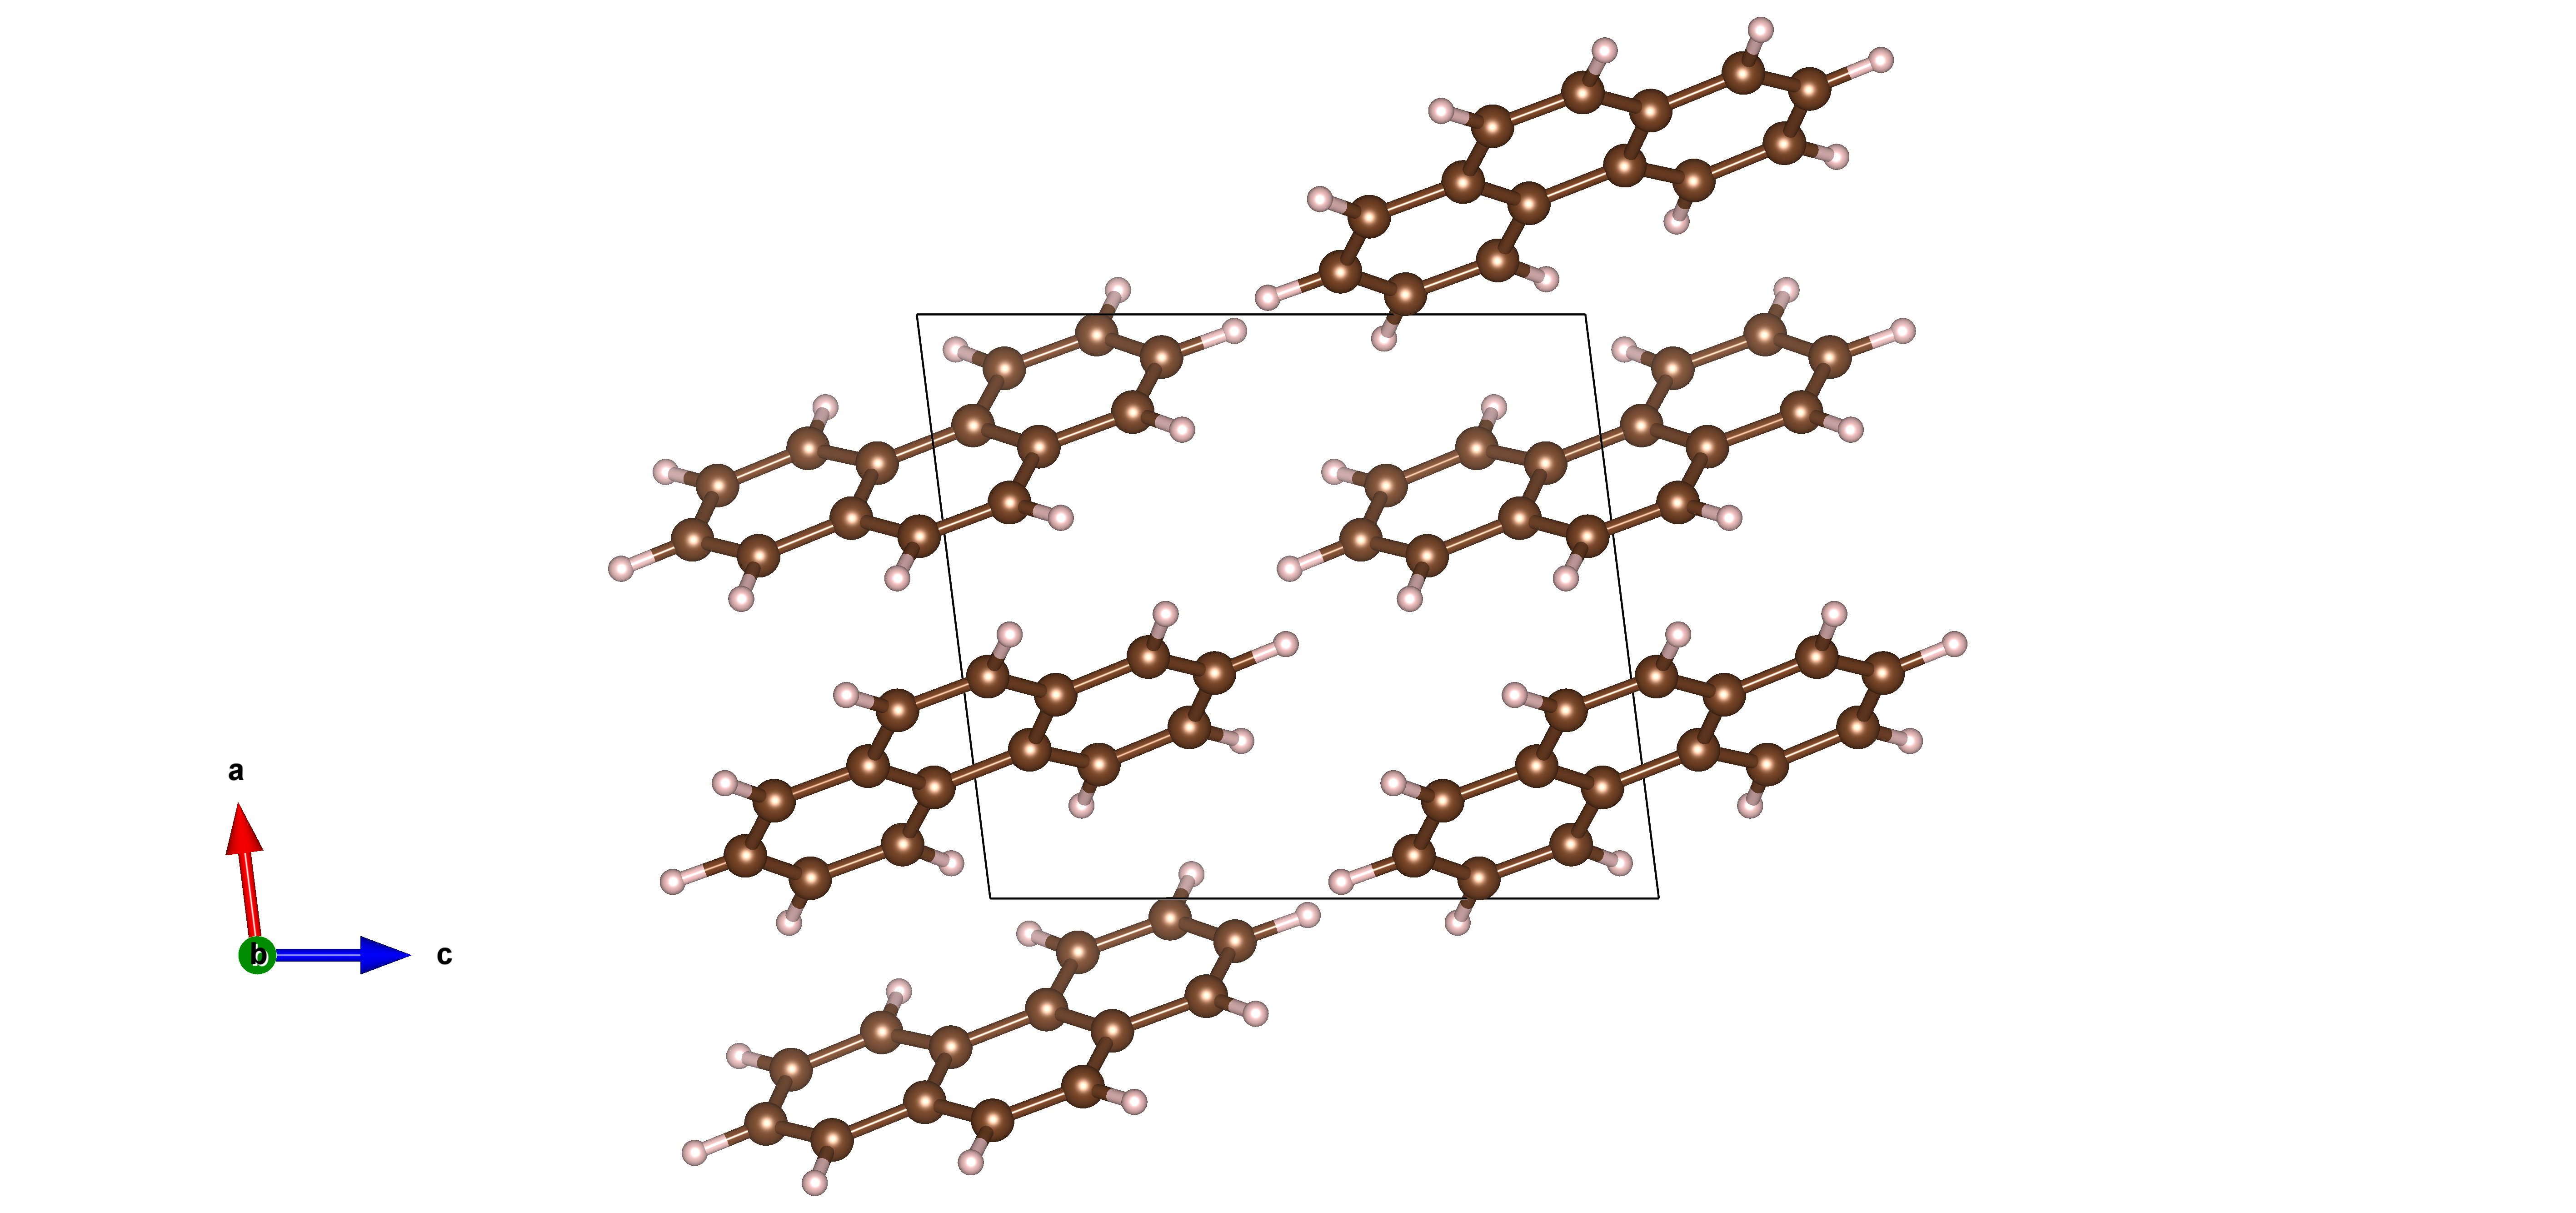
\includegraphics[scale=0.5]{image/Phenanthrene-b} & 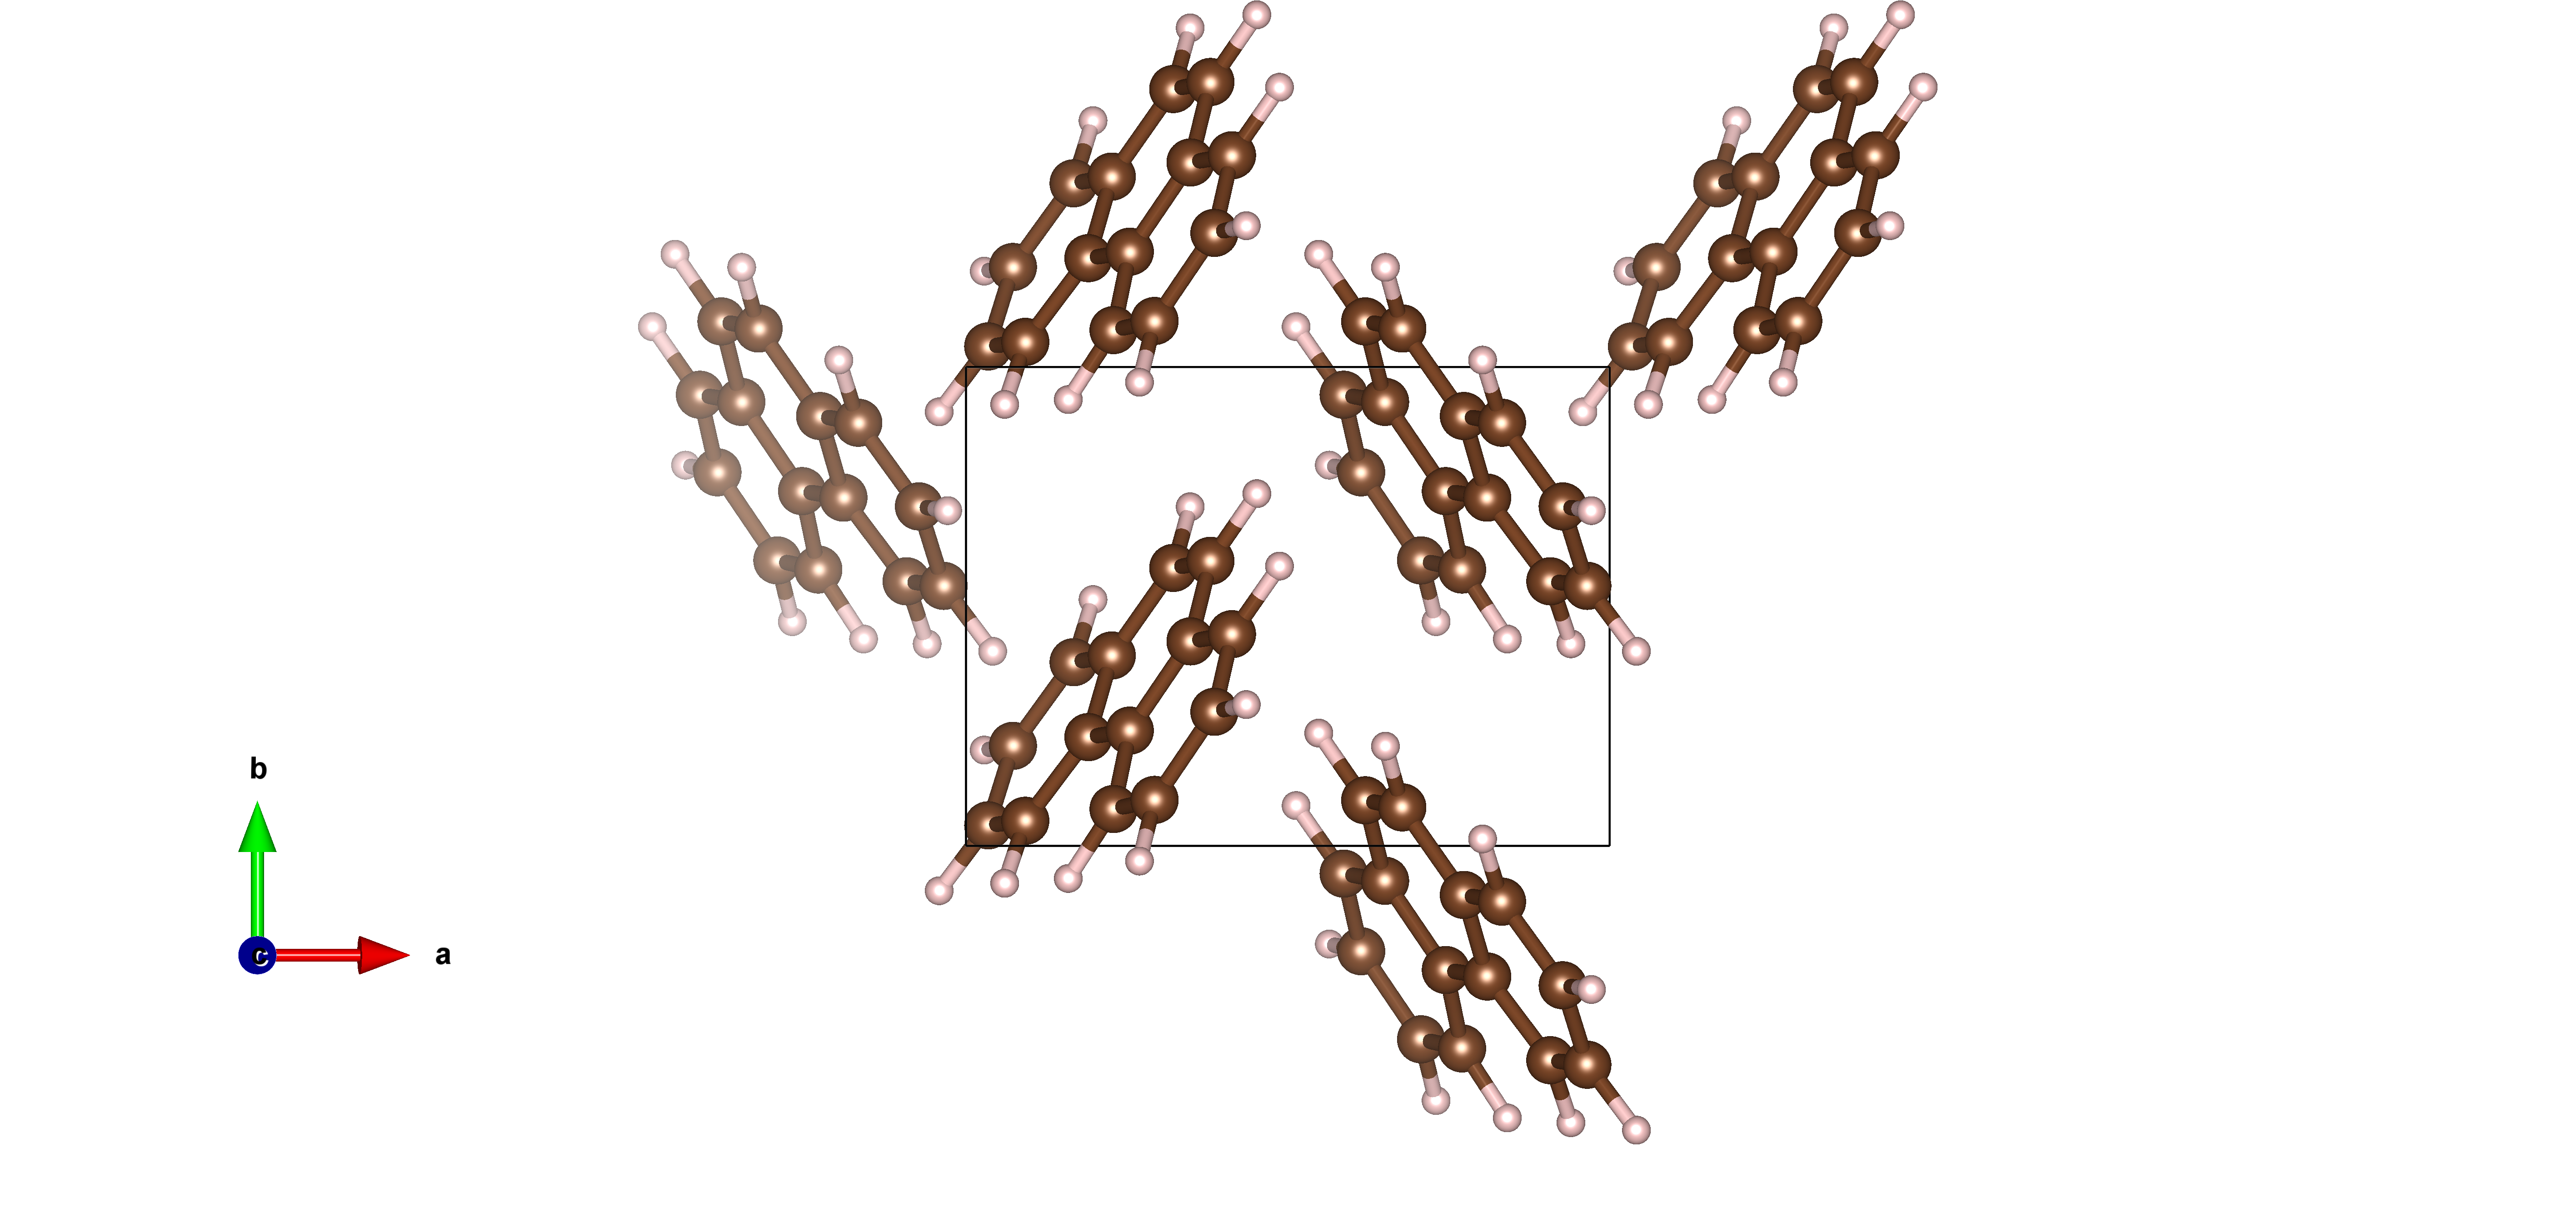
\includegraphics[scale=0.5]{image/Phenanthrene-c}  \\
 				\end{tabular}}
 				\caption{The \textit{ac} and \textit{ab} planes of Phenanthrene crystal} \label{fig-Phenansol}		
 			\end{center}
 		\end{figure}
 	
 	
 
 		
 		\begin{table}[H]
 			\caption{Lattice parameters of Phenanthrene molecule calculated in VASP code} \label{table-phenan}
 			\begin{center}
 				\begin{threeparttable}
 					\begin{tabular}{c c c c c c c}
 						\toprule
 						& \textbf{D2} & \textbf{D3} & \textbf{TS} & \textbf{TS-SCS} & \textbf{PBE*} & \textbf{Exp} ref\cite{fabbiani2006exploration} \\
 						\midrule
 						\textbf{a} & 7.91 (8.61) & 8.31 & 8.12 & 8.14 & 9.59 & 8.47\\
 						\textbf{b}& 6.04 (5.46) & 6.13 & 6.06 & 6.09 & 6.86 & 6.17\\
 						\textbf{c}& 9.30 (9.24) & 9.44 & 9.35 & 9.37 & 10.08 & 9.47\\
 						\textbf{$\beta$} & 95.89 (95.32) & 97.18 & 96.73 & 96.73 & 100.43 & 98.01\\
 						\textbf{Volume ($\AA^{3}$)}& 441.56 (432.83) & 477.42 & 456.69 & 460.92 & 651.81 & 489.72\\
 						\bottomrule
 					\end{tabular}
 					
 					\begin{tablenotes}
 						\item[*] without dispersion correction
 						\item[()] Parenthesis values were calculated with CRYSTAL program
 					\end{tablenotes}
 				\end{threeparttable}
 			\end{center}
 		\end{table}
 	
 	\begin{figure}[H]
 		\begin{center}
 			\resizebox{19cm}{!}{
 				\begin{tabular}{c c}
 				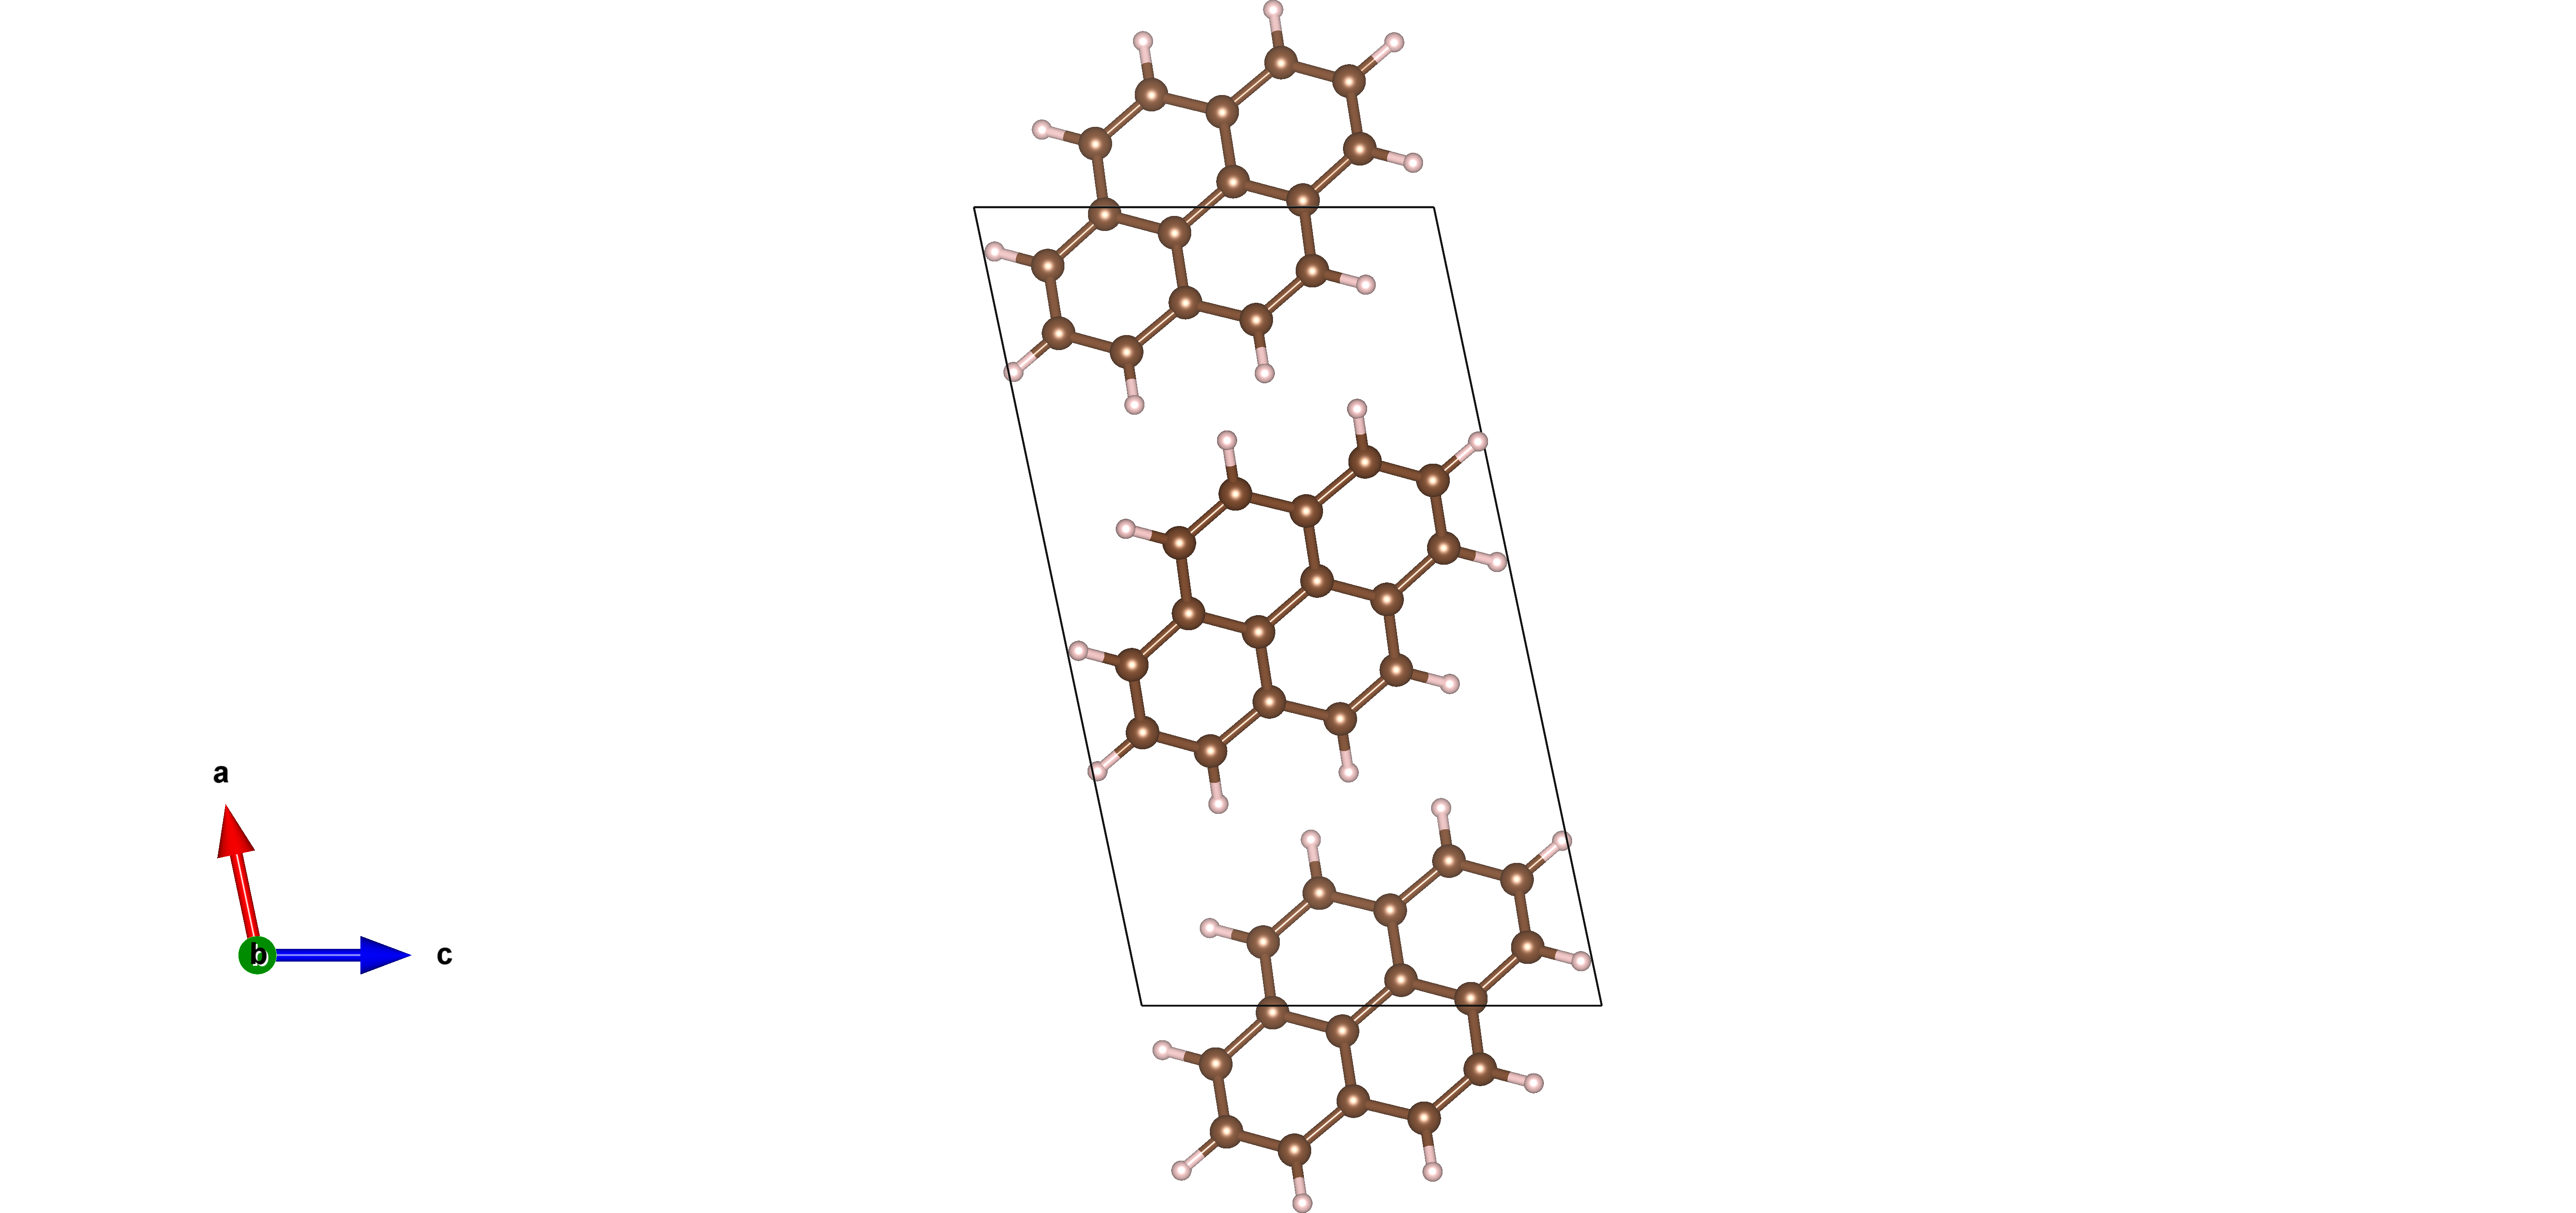
\includegraphics[scale=0.5]{image/Pyrene-b} &
 			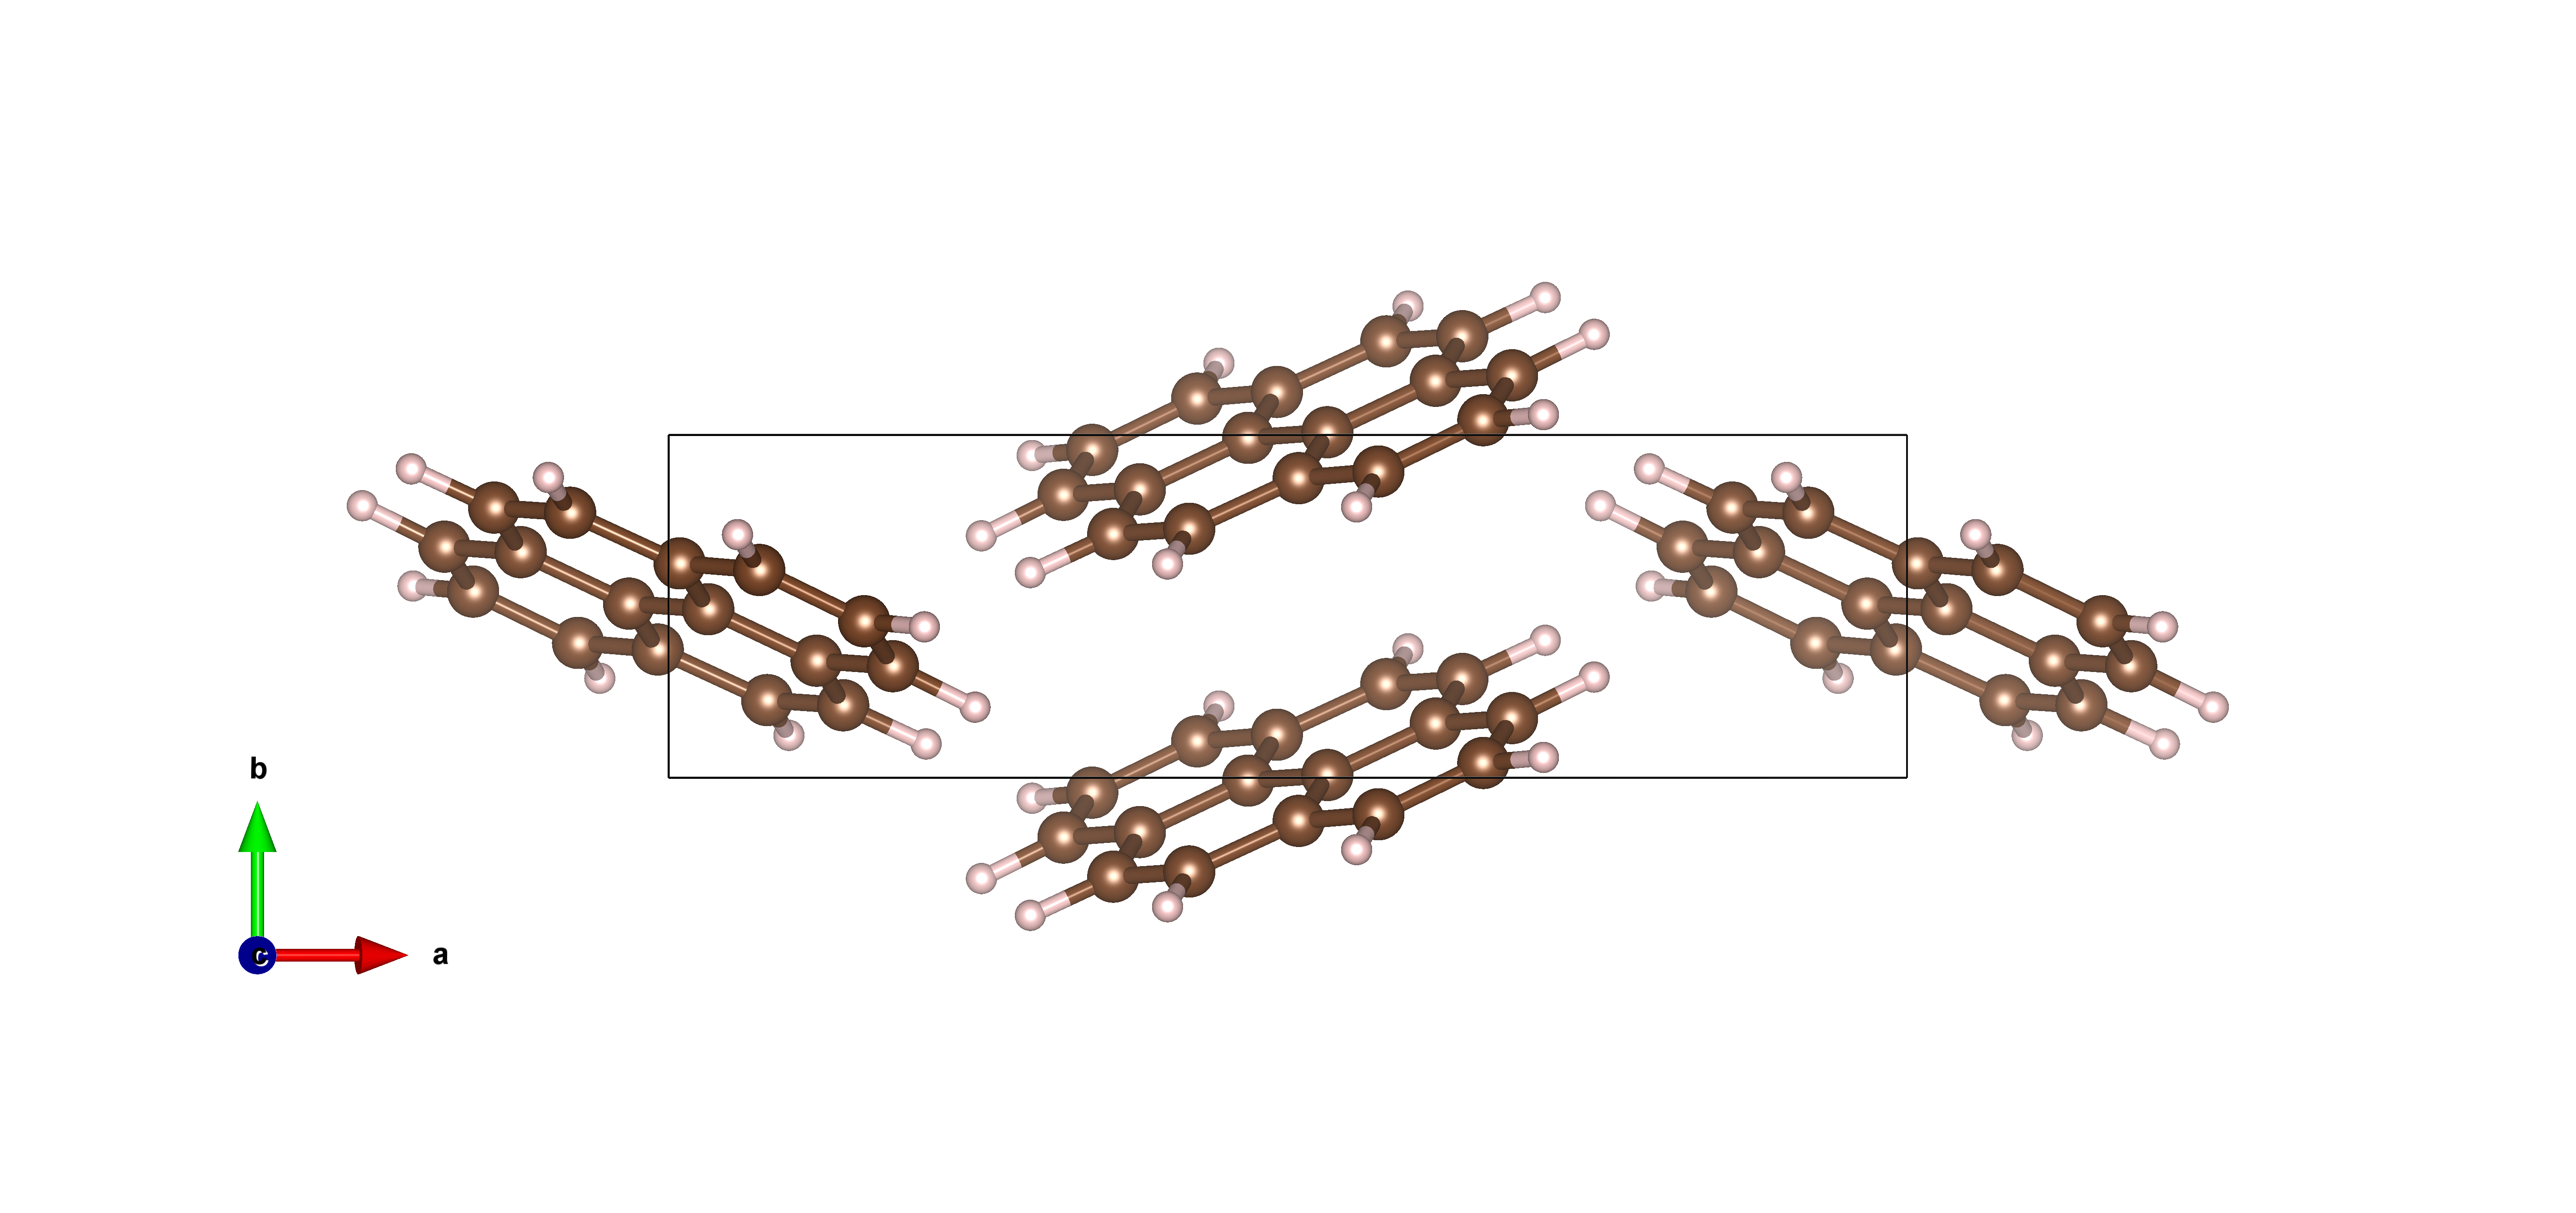
\includegraphics[scale=0.5]{image/Pyrene-c}  \\
 				\end{tabular}}
 			\caption{The \textit{ac} and \textit{ab} planes of Pyrene crystal}  \label{fig-pyrenesol}		
 			\end{center}
 		\end{figure}
 	
 
 	
 	\begin{table}[H]
 		\caption{Lattice parameters of Pyrene molecule calculated in VASP code}  \label{table-pyresol}
 		\begin{center}
 			\begin{threeparttable}
 			\begin{tabular}{c c c c c c c}
 				\toprule
 				& \textbf{D2} & \textbf{D3} & \textbf{TS} & \textbf{TS-SCS} & \textbf{PBE*} & \textbf{Exp} ref\cite{fabbiani2006exploration} \\
 				\midrule
 				\textbf{a} & 14.64 (13.22) & 14.93 & 15.02 & 15.10 & 16.17 & 15.35\\
 				\textbf{b}& 3.98 (4.41) & 4.04 & 3.93 & 4.00 & 4.64 & 3.85\\
 				\textbf{c}& 8.03 (8.01) & 8.42 & 8.43 & 8.42 & 9.10 & 8.65\\
 				\textbf{$\beta$} & 101.56 (98.28) & 101.88 & 102.02 & 101.83 & 103.82 & 103.03\\
 				\textbf{Volume ($\AA^{3}$)}& 470.08 (461.94) & 497.74 & 487.22 & 497.70 & 690.67 & 498.00\\
 				\bottomrule
 			\end{tabular}
 			
 			\begin{tablenotes}
 				\item[*] without dispersion correction
 				\item[()] Parenthesis values were calculated with CRYSTAL program
 			\end{tablenotes}
 		\end{threeparttable}
 		\end{center}
 	\end{table}
 	
 	
 	\begin{figure}[H]
 		\begin{center}
 			\resizebox{20cm}{!}{
 				\begin{tabular}{c c}
 				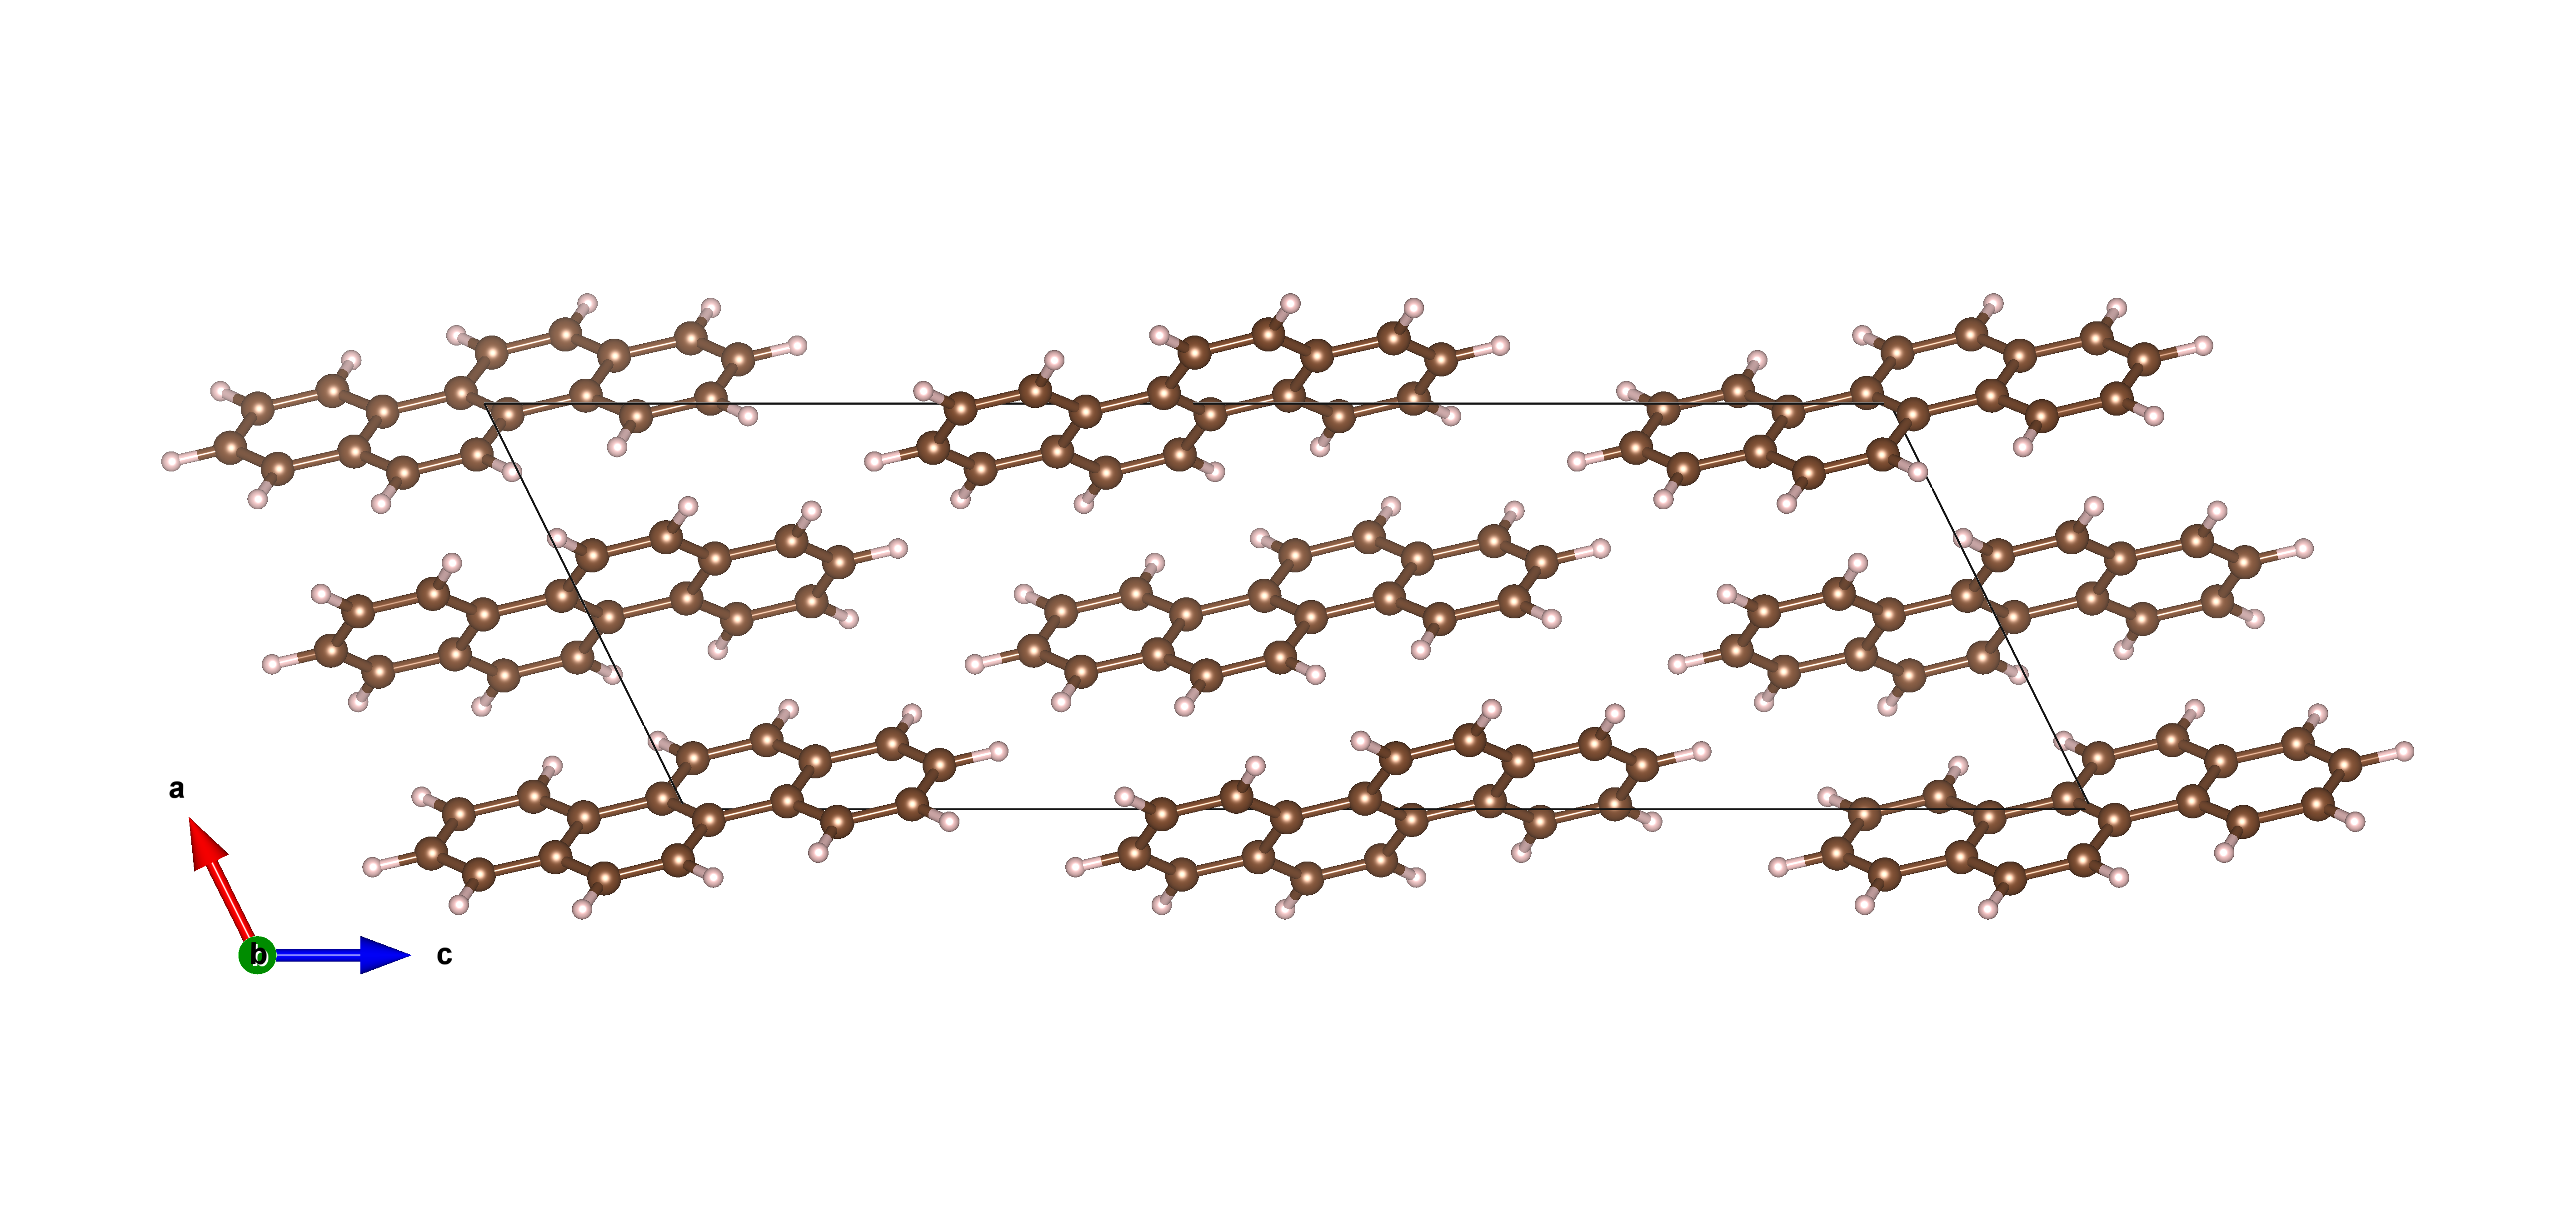
\includegraphics[scale=0.5]{image/Chrysene-b} & \includegraphics[scale=0.5]{image/Chrysene-C}  \\
 				\end{tabular}}
 			\caption{The \textit{ac} and \textit{ab} planes of Chrysene crystal}  \label{fig-chrysol}			
 			\end{center}
 		\end{figure}
 	
 
 	
 		
 		\begin{table}[H]
 			\caption{Lattice parameters of Chrysene molecule calculated in VASP code} \label{table-chrysol}
 			\begin{center}
 				\begin{threeparttable}
 				\begin{tabular}{c c c c c c c}
 					\toprule
 					& \textbf{D2} & \textbf{D3} & \textbf{TS} & \textbf{TS-SCS} & \textbf{PBE*} & \textbf{Exp} ref\cite{burns1960refinement} \\
 					\midrule
 					\textbf{a} & 7.85 (8.67) & 8.18 & 8.13 & 8.04 & 9.61 & 8.39\\
 					\textbf{b}& 6.08 (5.40) & 6.23 & 6.13 & 6.13 & 6.54 & 6.20\\
 					\textbf{c}& 25.10 (24.88) & 25.39 & 25.19 & 25.15 & 26.10 & 25.20\\
 					\textbf{$\beta$} & 117.05 (114.80) & 116.39 & 116.56 & 116.87& 115.76 & 116.20\\
 					\textbf{Volume ($\AA^{3}$)}& 1067.63 (1057.28)& 1157.58 & 1123.04 & 1105.90 & 1476.90 & 1175.00\\
 					\bottomrule
 				\end{tabular}
 				
 					\begin{tablenotes}
 						\item[*] without dispersion correction
 						\item[()] Parenthesis values were calculated with CRYSTAL program
 					\end{tablenotes}
 				\end{threeparttable}
 			\end{center}
 		\end{table}
 		
 	
 	\begin{figure}[H]
 		\begin{center}
 			\resizebox{20cm}{!}{
 				\begin{tabular}{c c}
 				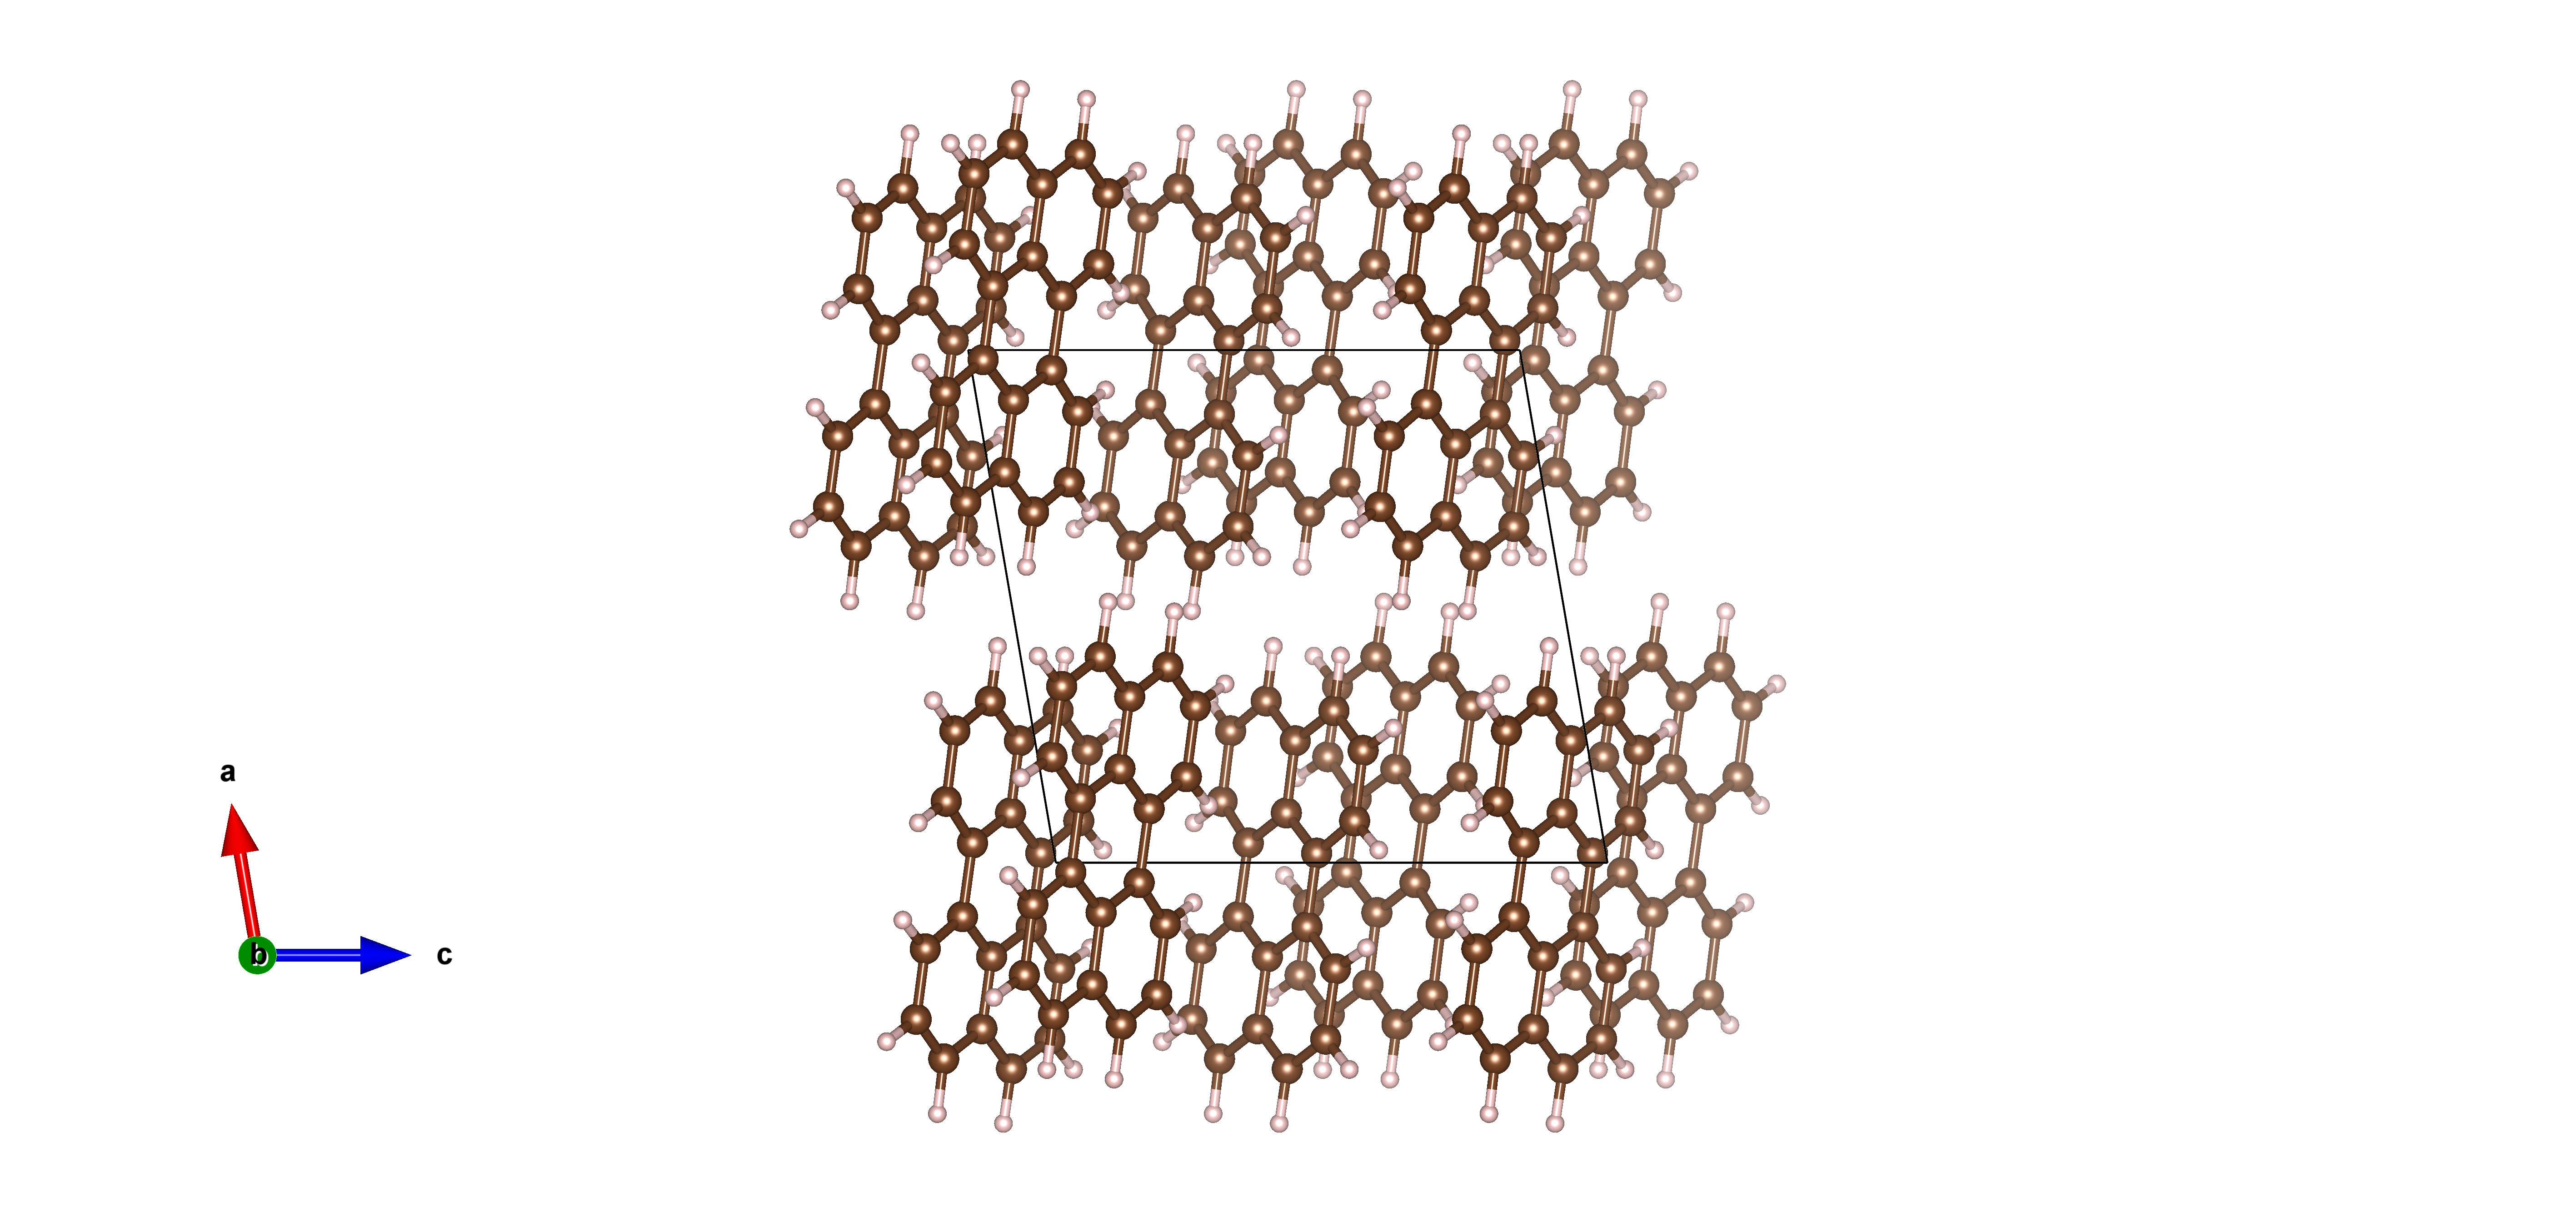
\includegraphics[scale=0.5]{image/Perylene-b} & 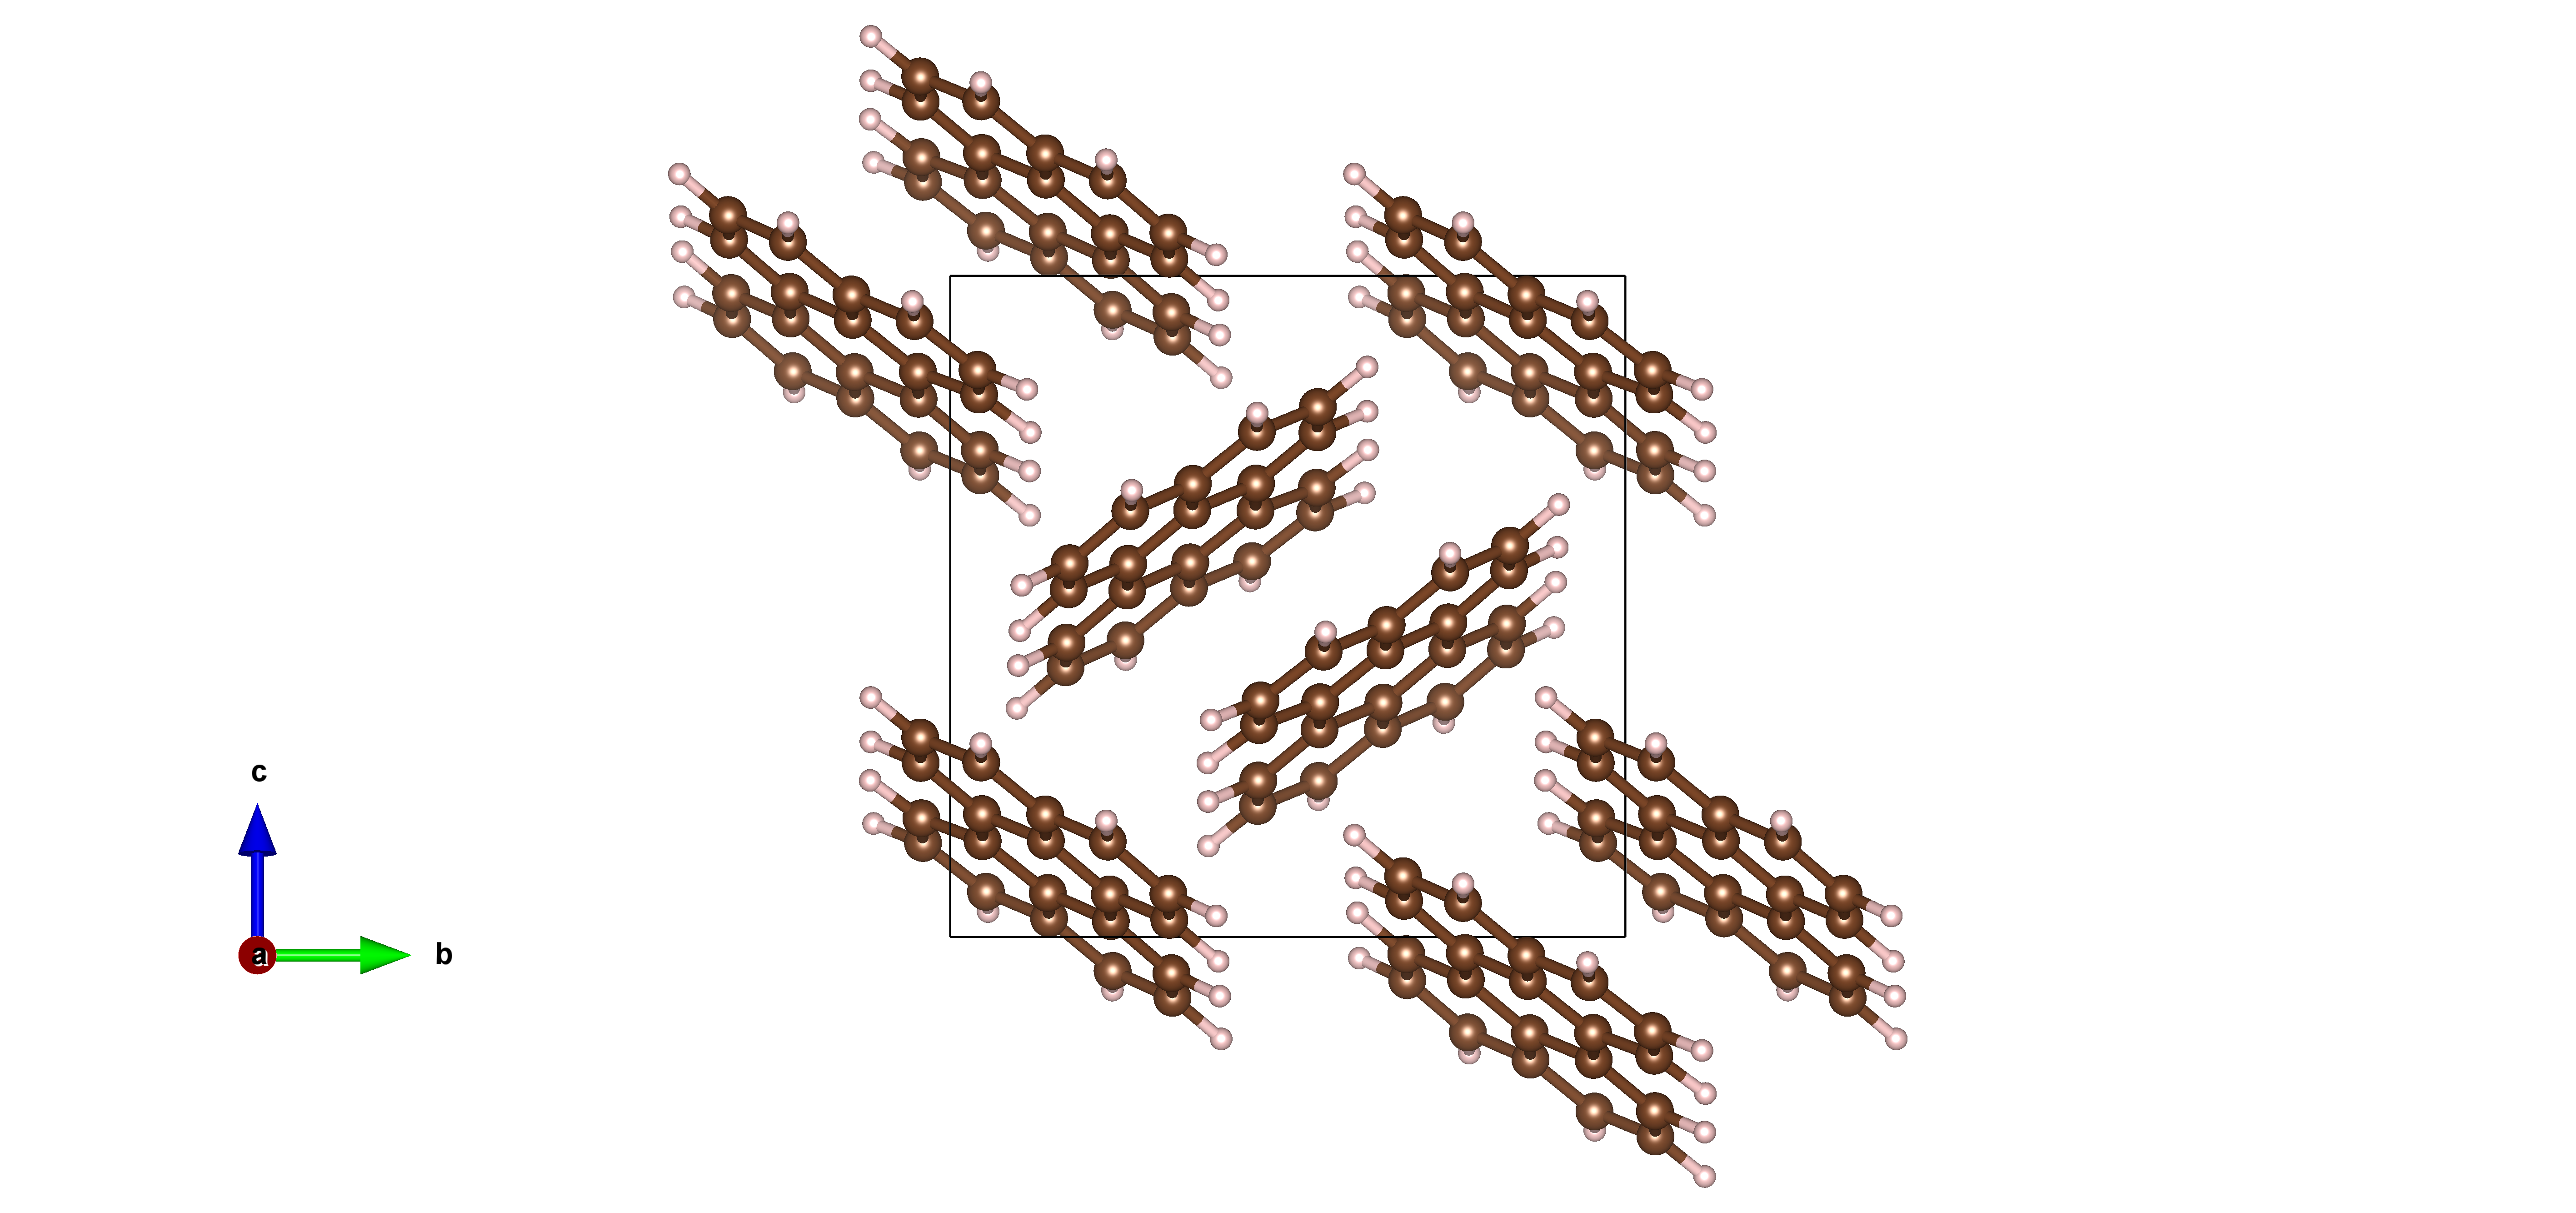
\includegraphics[scale=0.5]{image/Perylene-a} \\
 				\end{tabular}}
 			\caption{The \textit{ac} and \textit{bc} planes of Perylene crystal}  \label{fig-perylenesol}		
 			\end{center}
 		\end{figure}
 				
 					
 					
 					\begin{table}[H]
 						\caption{Lattice parameters of Perylene molecule calculated in VASP code} \label{table-perysol}
 						\begin{center}
 							\begin{threeparttable}
 								\begin{tabular}{c c c c c c c}
 									\toprule
 									& \textbf{D2} & \textbf{D3} & \textbf{TS} & \textbf{TS-SCS} & \textbf{PBE*} & \textbf{Exp} ref\cite{nather1998solvent}\\
 									\midrule
 									\textbf{a} & 9.99 (10.37)  & 10.29 & 10.21 & 10.27 & 10.80 &10.27 \\
 									\textbf{b}& 10.67 (10.27) & 11.00 & 10.91 & 10.98 & 11.41 & 10.84\\
 									\textbf{c}& 10.51 (10.91) & 10.92 & 10.64 & 10.83 & 12.85 & 11.28\\
 									\textbf{$\beta$} & 99.54 (103.62) & 99.70 & 99.25 &99.55 & 102.75 & 100.53 \\
 									\textbf{Volume ($\AA^{3}$)}& 1105.54 (1128.72)& 1218.72 & 1169.03 & 1203.94 & 1544.16 & 1234.29\\
 									\bottomrule
 								\end{tabular}
 								
 								\begin{tablenotes}
 									\item[*] without dispersion correction
 									\item[()] Parenthesis values were calculated with CRYSTAL program
 								\end{tablenotes}
 							\end{threeparttable}
 						\end{center}
 					\end{table}
 		
 		\begin{figure}[H]
 			\begin{center}
 				\resizebox{18cm}{!}{
 					\begin{tabular}{l}
 						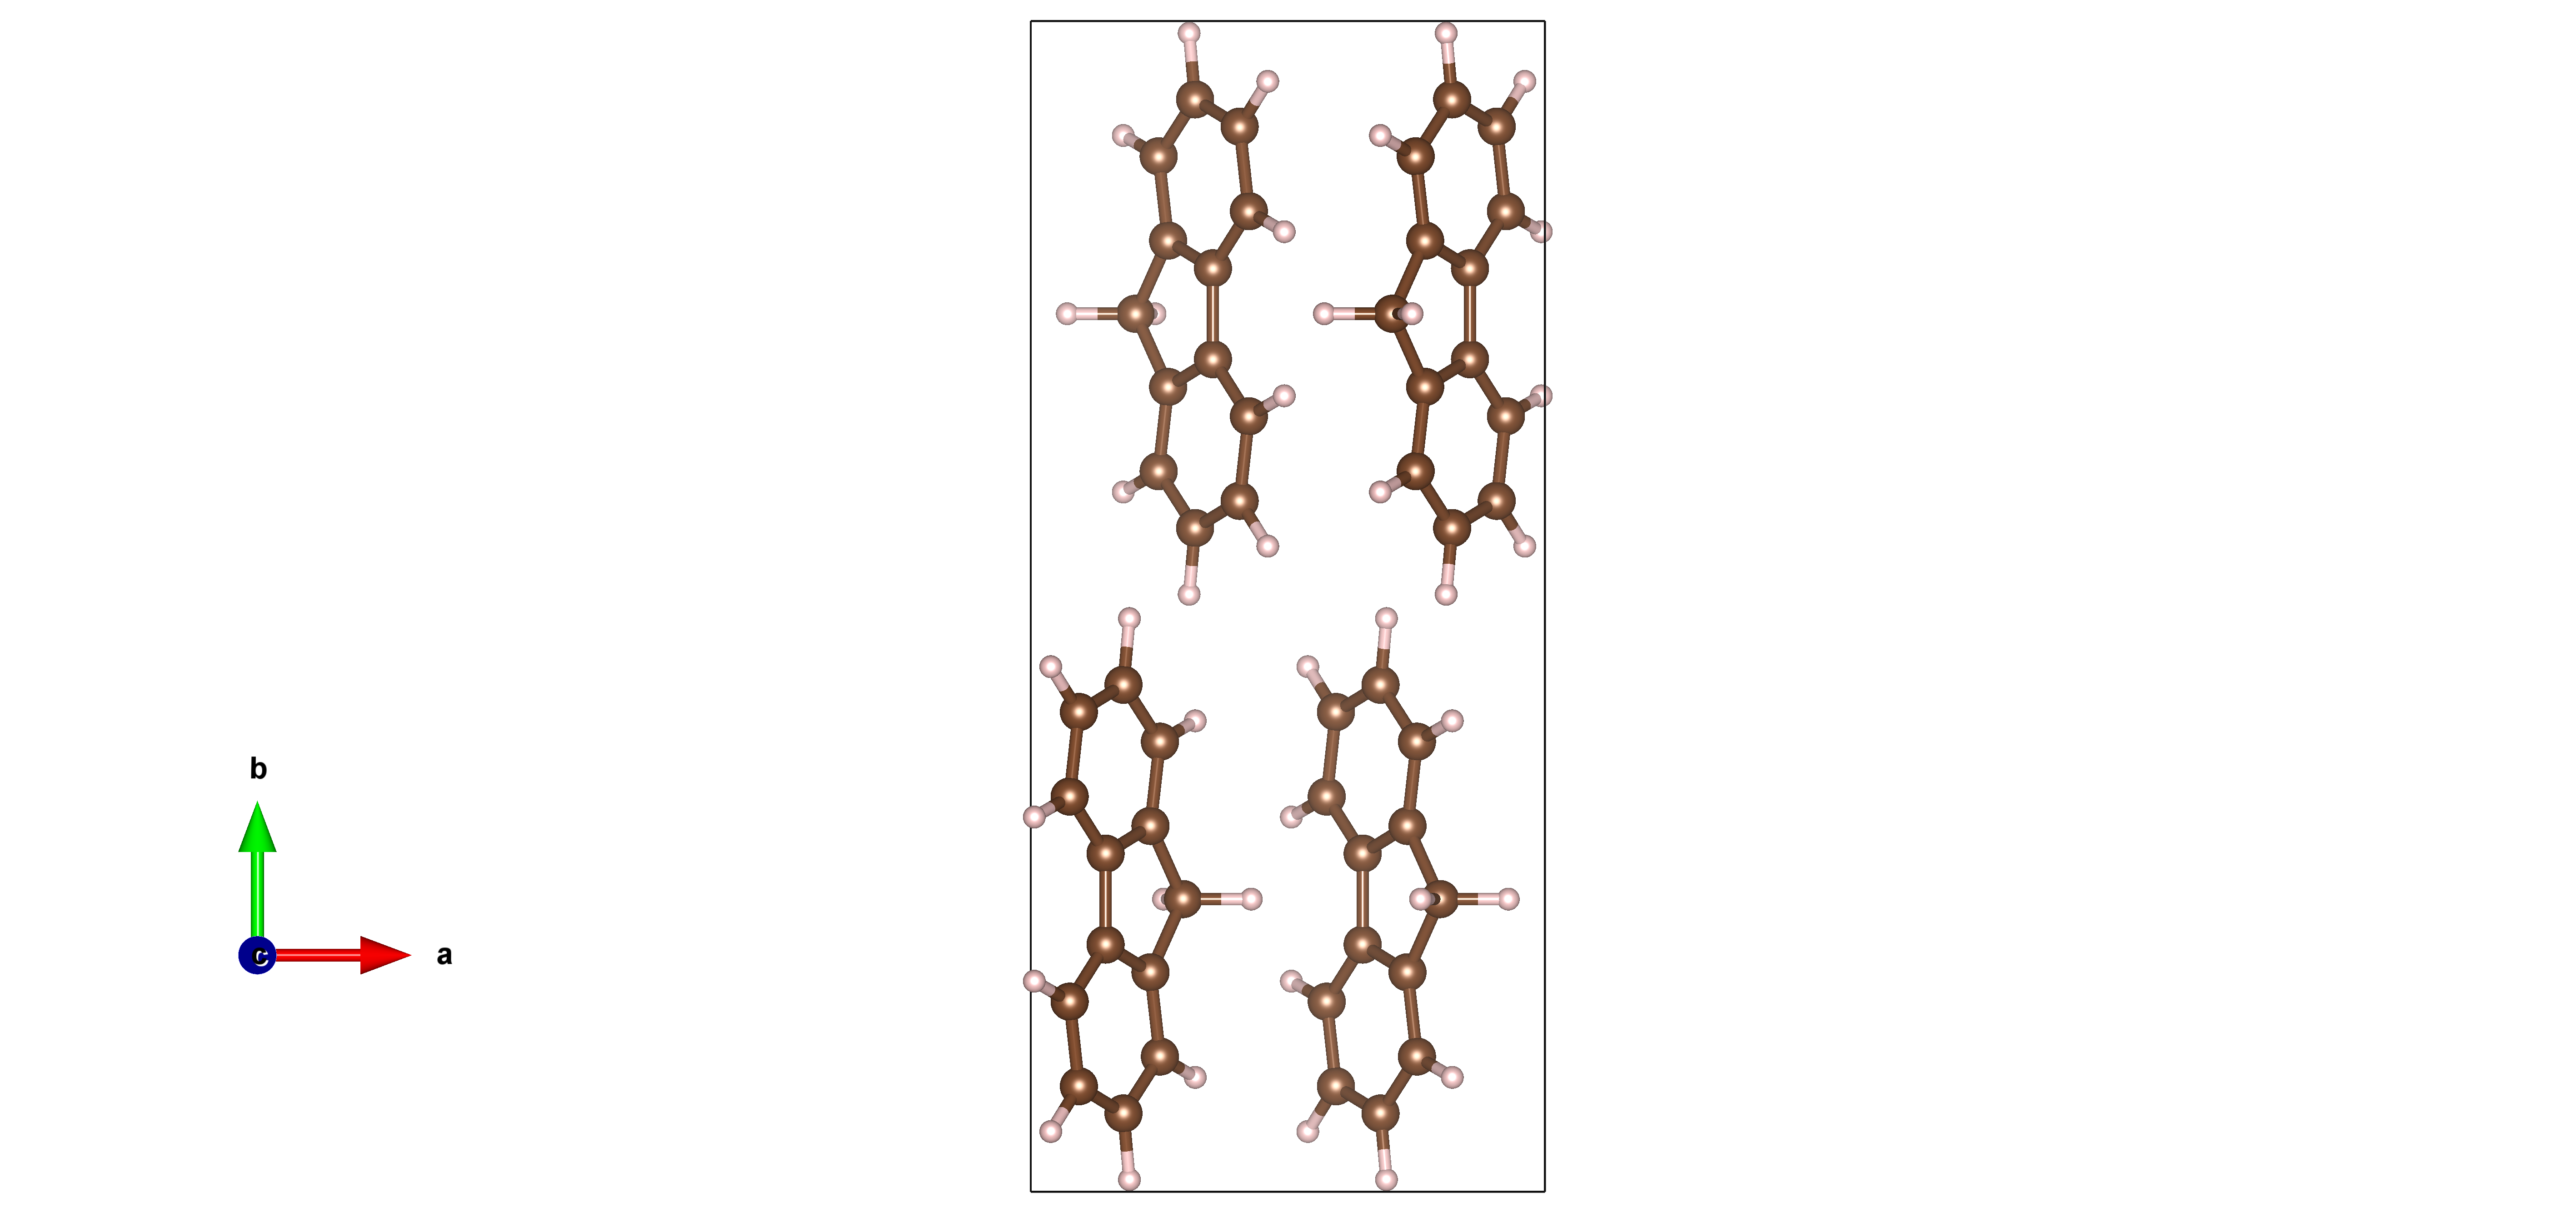
\includegraphics[scale=0.005]{image/Fluorene-c} \\
 						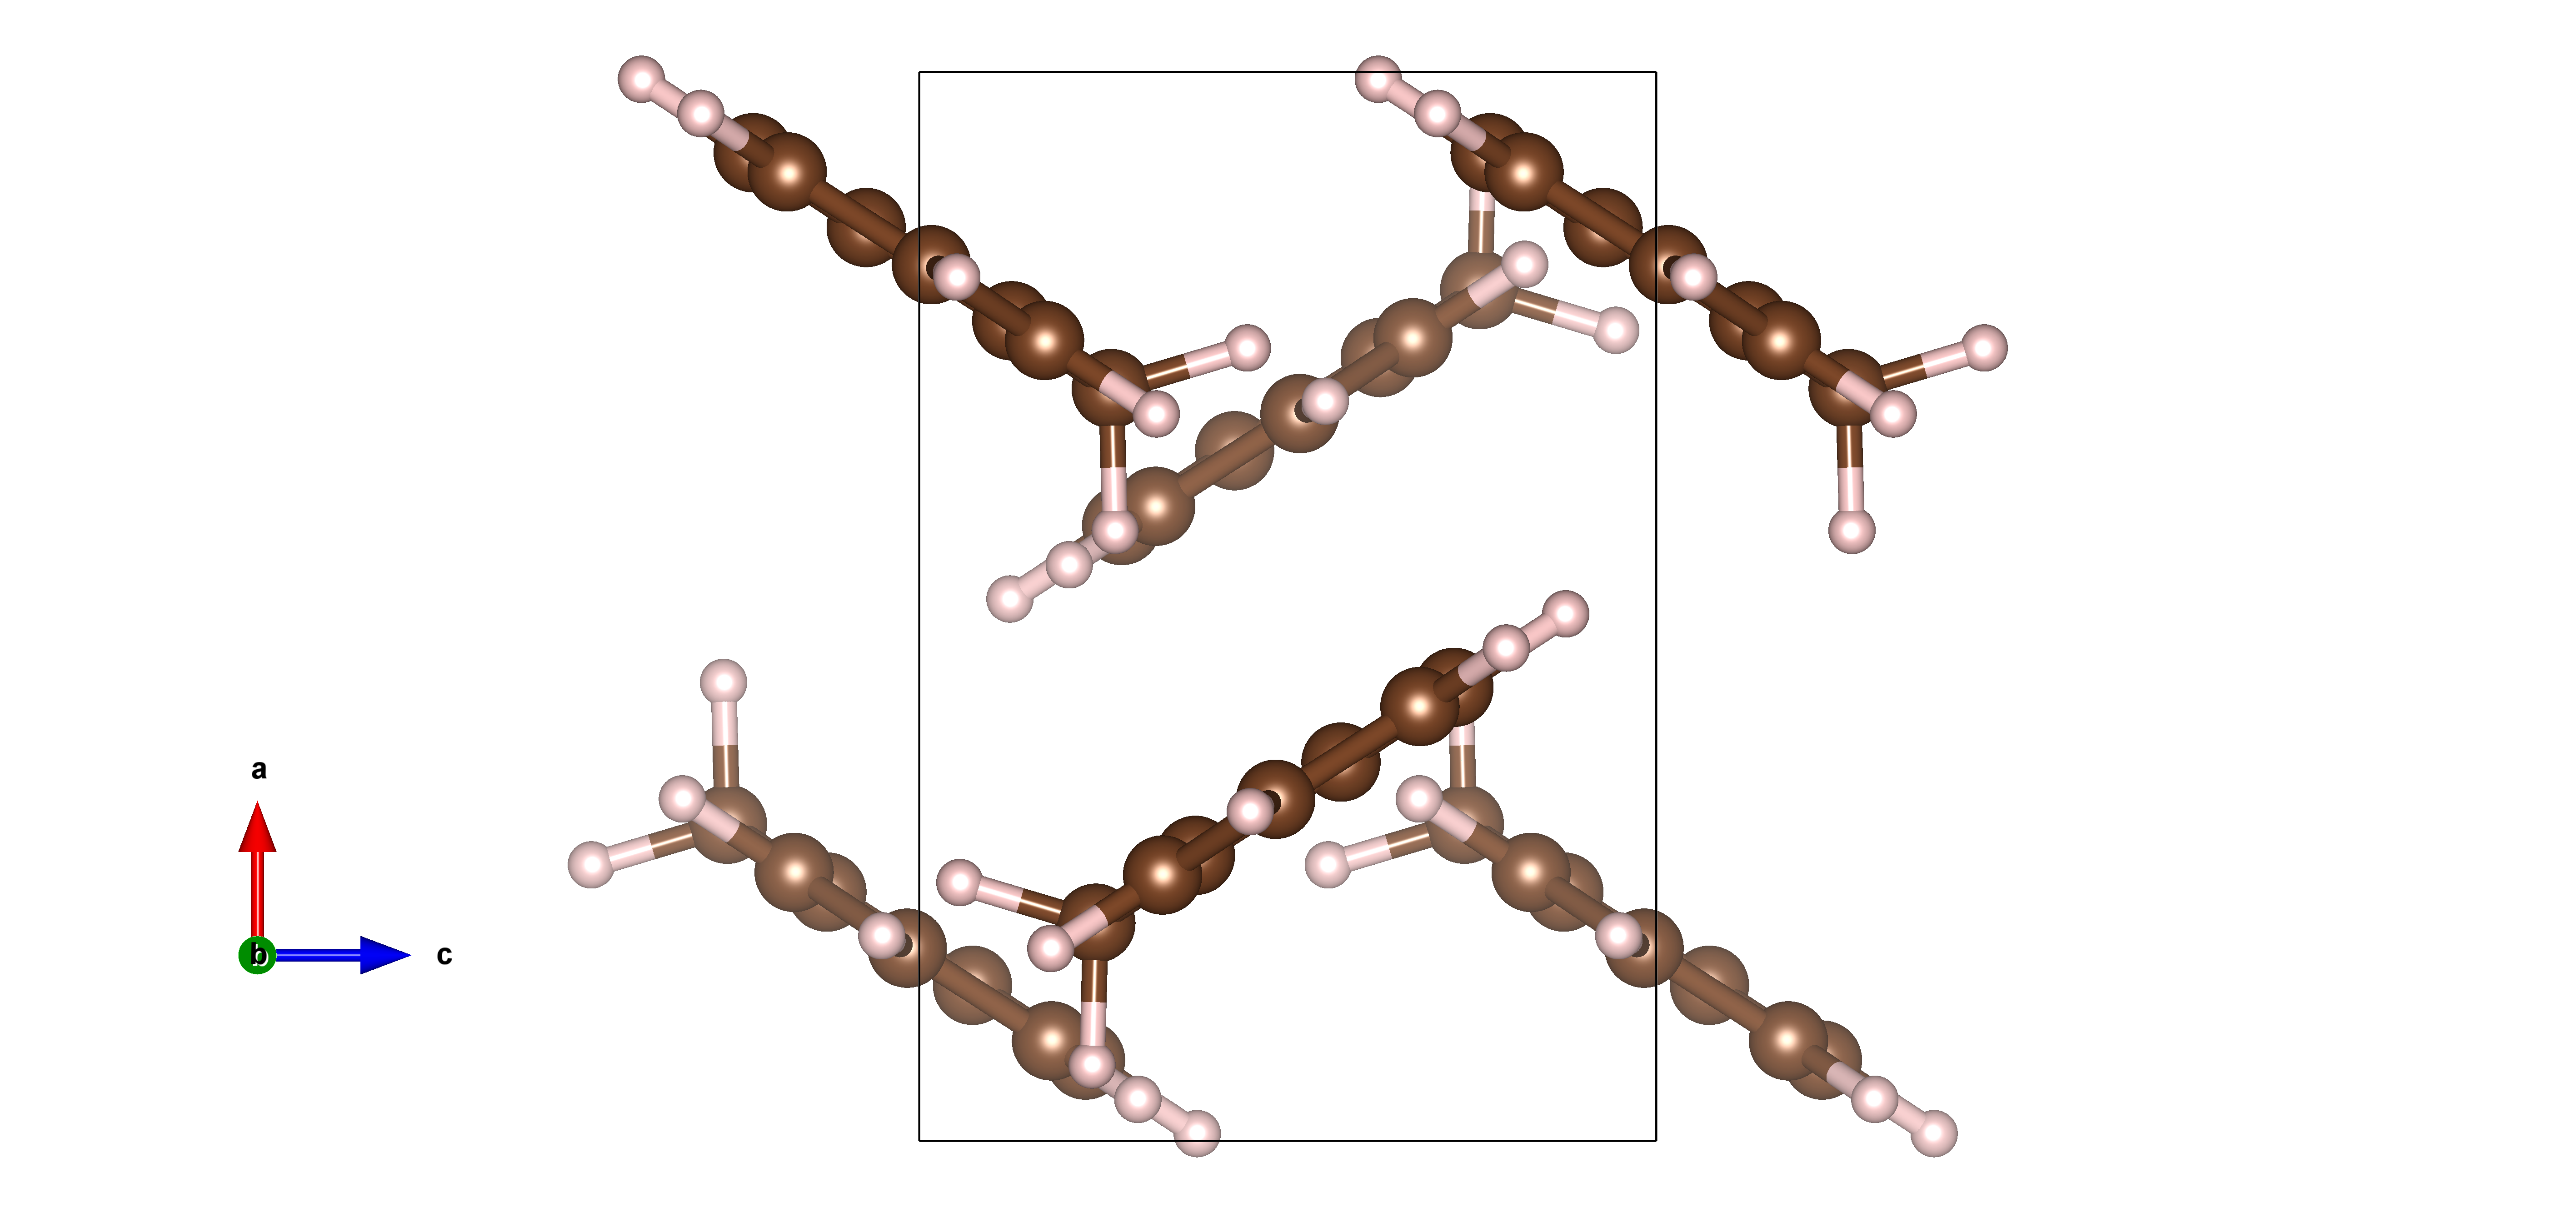
\includegraphics[scale=0.005]{image/Fluorene-b} \\
 					\end{tabular}}
 					\caption{The \textit{ab} and \textit{ac} planes of Fluorene crystal}  \label{fig-fluorenesol}
 				\end{center}
 			\end{figure}
 			 		 	
 			
 			
 				\begin{table}[H]
 					\caption{Lattice parameters of Fluorene molecule calculated in VASP code}  \label{table-fluorenesol}
 					\begin{center}
 						\begin{threeparttable}
 						\begin{tabular}{c c c c c c c}
 							\toprule
 							& \textbf{D2} & \textbf{D3} & \textbf{TS} & \textbf{TS-SCS} & \textbf{PBE*} & \textbf{Exp} ref\cite{belsky1984fluorene}\\
 							\midrule
 							\textbf{a} & 7.96 (8.25) & 8.30 & 8.08 & 8.16 & 9.77 & 8.48 \\
 							\textbf{b}& 18.40 (18.61) & 18.90 & 18.77 & 18.82 & 19.54 & 18.92\\
 							\textbf{c}& 5.54 (5.26) & 5.72 & 5.64 & 5.68 & 6.16 & 5.72\\
 							\textbf{Volume ($\AA^{3}$)}& 810.91 (807.12) & 897.69 & 855.73 & 871.59 & 1176.23 & 916.60\\
 							\bottomrule
 						\end{tabular}
 						
 						\begin{tablenotes}
 							\item[*] without dispersion correction
 							\item[()] Parenthesis values were calculated with CRYSTAL program
 						\end{tablenotes}
 					\end{threeparttable}
 					\end{center}
 				\end{table}
 				

 	\begin{spacing}{1.1}		
 		\begin{table}[H]
 			\caption{ Calculated vibrational frequencies (cm$^{-1}$) of the monomer, dimer and solid-state (PBE Phenanthrene system).}  \label{table-freqPhen}
 			\begin{center}
 				\begin{threeparttable}
 				\begin{tabular}{c c c c c}
 					\toprule
 					\multicolumn{2}{p{4.5cm}}{\centering \textbf{Monomer}} & \textbf{Dimer} & \multicolumn{1}{p{4cm}}{\centering \textbf{Experimental} \\ ref \cite{godec1976interpretation}/ ref \cite{bree1972vibrational}} & \textbf{VASP/CRYSTAL}\\
 					Assignment & $\nu$(cm$^{-1}$) & $\nu$(cm$^{-1}$) & $\nu$(cm$^{-1}$) & $\omega$(cm$^{-1}$) \\
 					& Int(km/mol) & Int(km/mol) & & Int(km/mol) \\
 					\midrule
 					&  &  \textit{11 (0.003)}& & \\
 					&  & \textit{14 (0.005)} &  & \\
 					&  & \textit{42 (0.02)}&  & \textit{57 (0.4)}\\
 					&  & \textit{69 (0.2)} &  & \textit {63 (1.05)}\\
 					&  & \textit{74 (0.06)}&  & \textit{73 (0.01)}\\
 					&  & \textit{81 (0.02)} & 89 & \textit{88 (0.91)} \\
 					&   &    &    &  \textit{93 (1.88)}\\
 					\\
 					\multirow{2}{2cm}{\centering $\nu_{1}$}& \multirow{2}{2cm}{\centering 99 (0)} & 102 (1.04) & \multirow{2}{2cm}{\centering 97}& 103 (0.34)\\
 					&   & 113 (0.61)  &    & 118 (1.88)\\
 					\multirow{2}{2cm}{\centering $\nu_{2}$} & \multirow{2}{2cm}{\centering 103 (1.06)}& 123 (0.44)& \multirow{1}{2cm}{\centering 124/127} & 119 (0.05)\\
 					&  &  126 (0.02) & 143 (sh)  & 127 (0.53)\\
 					\multirow{2}{2cm}{\centering $\nu_{3}$} &  \multirow{2}{2cm}{\centering 235 (5.01)}& 239 (9.23)& \multirow{2}{2cm}{\centering 229(w)/ \\ 233 (s)} & 231 (0.44)\\
 					&  & 244 (0.35)  &   & 241 (0.86)\\
 					\multirow{2}{2cm}{\centering $\nu_{4}$} & \multirow{2}{2cm}{\centering 251 (0)} & 250 (0.31) & \multirow{4}{4cm}{\centering 248(s)/ \\ 250 (m)} & 241 (0.12) \\
 					&  &  255 (0.5)&   & 243 (4.21)\\
 					\multirow{2}{2cm}{\centering $\nu_{5}$} & \multirow{2}{2cm}{\centering 255 (0.43)} & 255 (0.21)&  & 250 (2.51)\\
 					&   &  259 (0.13) &  & 251 (0.04) \\
 					&   &   & 289(w) & \\
 					&  &    &  \multirow{2}{2cm}{\centering 398(vw)/ \\ 395 (vw)}& 394 (0.34)\\
 					&  &    &   & 395 (0.11)\\
 					\multirow{2}{2cm}{\centering $\nu_{6}$} & \multirow{2}{2cm}{\centering 412 (0)} & 411 (0.03)& \multirow{2}{2cm}{\centering 409(w)/ \\ 408 (ms)} & 403 (0.1)\\
 					&   &  415 (0.28) &  & 408 (0.63)\\
 					\bottomrule	    
 				\end{tabular}
 				
 				\begin{tablenotes}
 					\item[] Italic: Intermolecular modes
 				\end{tablenotes}
 			\end{threeparttable}
 			\end{center}
 		\end{table}
 	\end{spacing}
 		
 		
 		\begin{table}[H]
 			\caption{ Calculated vibrational frequencies (cm$^{-1}$) of the monomer, dimer and solid-state (PBE Pyrene system).}  \label{table-freqPyr}
 			\begin{center}
 				\begin{threeparttable}
 				\begin{tabular}{c c c c c}
 					\toprule
 					\multicolumn{2}{p{4.5cm}}{\centering \textbf{Monomer}} & \textbf{Dimer} & \multicolumn{1}{p{4cm}}{\centering \textbf{Experimental} \\ ref \cite{michaelian2009far}} & \textbf{VASP/CRYSTAL}\\
 					Assignment & $\nu$(cm$^{-1}$) & $\nu$(cm$^{-1}$) & $\nu$(cm$^{-1}$) & $\omega$(cm$^{-1}$) \\
 					& Int(km/mol) & Int(km/mol) & & Int(km/mol) \\
 					\midrule
 					&  &  \textit{17 (<0.01)}& & \\
 					&  & \textit{30 (0)} &  & \\
 					&  & \textit{40 (0)}&  & \\
 					&  & \textit{69 (0.01)} &  & \textit {50 (0.05)}\\
 					&  & \textit{94 (0.01)}& 83 (m) & \textit{94 (5.98)}\\
 					&  & \textit{95 (0)} &  & \\
 					\\
 					\multirow{2}{2cm}{\centering $\nu_{1}$}& \multirow{2}{2cm}{\centering 100 (0.66)} & \multirow{2}{2cm}{\centering 115 (1.60)} & \multirow{2}{2cm}{\centering 98 (m)}& \textit{97 (2.31)}\\
 					&   &   &    & 105 (0.33)\\
 					&   &   &  121 (w)& \\
 					&   &   &  138 (vw) & 135 (2.71)\\
 					\multirow{2}{2cm}{\centering $\nu_{2}$} & \multirow{2}{2cm}{\centering 157 (0)}& \multirow{2}{2cm}{\centering 162 (0.03)}& \multirow{2}{2cm}{\centering 157 (w)} & 157 (0.77)\\
 					&  &   &   & 162 (4.27)\\
 					&  &   & 181 (vw) & \\
 					&   &   & 197 (vw) &  \\
 					\multirow{2}{2cm}{\centering $\nu_{3}$} &  \multirow{2}{2cm}{\centering 220(12.56)}& \multirow{2}{2cm}{\centering 225(24.34)}& \multirow{2}{2cm}{\centering 221 (m)} & 211 (4.64)\\
 					&  &   &   & 231 (7.89)\\
 					$\nu_{4}$ & 260 (0) & 264 (0) & \multirow{2}{2cm}{\centering 260 (w)} & 261 (0) \\
 					$\nu_{5}$ & 269 (0) & 275 (0.18)&  & 264 (0)\\
 					&   &   & 284 (w) &  \\
 					&   &   & 305 (vw) & \\
 					&  &   & 323 (w) &  \\
 					\multirow{2}{2cm}{\centering $\nu_{6}$} & \multirow{2}{2cm}{\centering 370 (1.54)} & \multirow{2}{2cm}{\centering 370 (2.05)}& \multirow{2}{2cm}{\centering 353 (m)} & 349 (0.53)\\
 					&   &   &   & 350 (1.71)\\
 					\multirow{2}{2cm}{\centering $\nu_{7}$} & \multirow{2}{2cm}{\centering 412 (0)}& \multirow{2}{2cm}{\centering 416(0.004)} & \multirow{2}{2cm}{\centering 396 (vw)}& 391 (0.82)\\
 					&   &   &   & 394 (0.04)\\
 					\bottomrule	    
 				\end{tabular}
 				
 				\begin{tablenotes}
 					\item[] Italic: Intermolecular modes
 				\end{tablenotes}
 			\end{threeparttable}
 			\end{center}
 		\end{table}
 				
 	
 	\begin{spacing}{1.1}
 		\begin{table}[H]
 			\caption{ Calculated vibrational frequencies (cm$^{-1}$) of the monomer, dimer and solid-state (PBE Chrysene system).}  \label{table-freqChry}
 			\begin{center}
 				\begin{threeparttable}
 				\begin{tabular}{c c c c c}
 					\toprule
 					\multicolumn{2}{p{4.5cm}}{\centering \textbf{Monomer}} & \textbf{Dimer} & \multicolumn{1}{p{4cm}}{\centering \textbf{Experimental} \\ ref \cite{zhang1996far}} & \textbf{VASP/CRYSTAL}\\
 					Assignment & $\nu$(cm$^{-1}$) & $\nu$(cm$^{-1}$) & $\nu$(cm$^{-1}$) & $\omega$(cm$^{-1}$) \\
 					& Int(km/mol) & Int(km/mol) & & Int(km/mol) \\
 					\midrule
 					&  &  \textit{15 (0.002)}& & \\
 					&  & \textit{26 (0.02)} &  & \\
 					&  & \textit{34 (0)}&  & \textit{41 (0.01)}\\
 					$\nu_{1}$ & 50 (0.21) & 53 (0.2) &  & 69 (0.11)\\
 					$\nu_{2}$ &79 (0.34)  & 76 (0.02)&  & \\
 					&  & \textit{86 (0)} &  &  \\
 					&   &  \textit{88 (0.18)}  &    &  \textit{112 (2.88)}\\
 					&   & \textit{95 (0.95)}&  & \textit{114 (3.19)}\\
 					\\
 					&   &  100 (0) &  & \multirow{2}{2cm}{\centering 100 (0.09)}\\
 					&   &  115 (0)&  &  \\
 					\multirow{2}{2cm}{\centering $\nu_{3}$}& \multirow{2}{2cm}{\centering 138 (0)} & 145 (0) & & 134 (0.63)\\
 					&   & 157 (0.01)  &    & 158 (0.26)\\
 					\multirow{2}{2cm}{\centering $\nu_{4}$} & \multirow{2}{2cm}{\centering 181 (0)} & 190 (0) &  &   \\
 					&   &  194 (0.13) &  &  \\
 					\multirow{2}{2cm}{\centering $\nu_{5}$} & \multirow{2}{2cm}{\centering 192 (0.52)}& 194 (0.73)&  & \multirow{2}{2cm}{\centering 189 (0.82)}\\
 					&   &  195 (0)&  &  \\
 					\multirow{2}{2cm}{\centering $\nu_{6}$} & \multirow{2}{2cm}{\centering 243 (7.50)} & 248 (14.70) & \multirow{2}{2cm}{\centering 232} & 247 (1.18)\\
 					&   &  254 (0)&  & 251 (10.72)\\
 					\multirow{2}{2cm}{\centering $\nu_{7}$} & \multirow{2}{2cm}{\centering 300 (0)} & 302 (0) &  &  \\
 					&   & 303 (0.06)&  & \\
 					\multirow{2}{2cm}{\centering $\nu_{8}$} & \multirow{2}{2cm}{\centering 301 (0.24)} & 308 (0) &  & 292 (2.56)\\
 					&  &  309 (0.44)&  & 295 (0.09)\\
 					\multirow{2}{2cm}{\centering $\nu_{9}$} & \multirow{2}{2cm}{\centering 396 (0)} & 396 (0.005) &   &  \\
 					&   & 396 (0) &  & \\
 					\bottomrule	    
 				\end{tabular}
 				
 				\begin{tablenotes}
 					\item[] Italic: Intermolecular modes
 				\end{tablenotes}
 			\end{threeparttable}
 			\end{center}
 		\end{table}
 	\end{spacing}
 	
 	
 	\begin{spacing}{1.1}
 		\begin{table}[H]
 			\caption{ Calculated vibrational frequencies (cm$^{-1}$) of the monomer, dimer and solid-state (PBE Perylene system).}  \label{table-freqPery}
 			\begin{center}
 				\begin{threeparttable}
 					\resizebox{17cm}{!}{
 					\begin{tabular}{c c c c c}
 						\toprule
 						\multicolumn{2}{p{4.5cm}}{\centering \textbf{Monomer}} & \textbf{Dimer} & \multicolumn{1}{p{4cm}}{\centering \textbf{Experimental} \\ ref \cite{michaelian2009far}} & \textbf{VASP/CRYSTAL}\\
 						Assignment & $\nu$(cm$^{-1}$) & $\nu$(cm$^{-1}$) & $\nu$(cm$^{-1}$) & $\omega$(cm$^{-1}$) \\
 						& Int(km/mol) & Int(km/mol) & & Int(km/mol) \\
 						\midrule
 						\multirow{2}{2cm}{\centering $\nu_{1}$}& \multirow{2}{2cm}{\centering 17 (0.00)}& 14 (0.001) &   &   \\
 						&   &   33(0.00) &   &  \\
 						&  & \textit{31 (0.00)}&  & \textit{39 (0.12)}\\
 						&  & \multirow{2}{2cm}{\centering \textit{35 (0.00)}} &  & \textit{45 (0.06)}\\
 						&  &   &   &  \textit{48 (0.17)}\\	
 						&  & \textit{73 (0.10)} & \multirow{2}{2cm}{\centering 83 (m)} & \multirow{2}{2cm}{\centering \textit{87 (3.61)}}\\
 						&  &  \textit{84 (0.15)} &  &  \\
 						&   &  \textit{89 (0.00)}&   &  \\
 						\\
 						\multirow{3}{3cm}{\centering $\nu_{2}$}& \multirow{3}{3cm}{\centering 100 (1.00)} & \multirow{3}{3cm}{\centering 110 (2.00) \\ 126 (0.00)} & \multirow{3}{3cm}{\centering 98 (m)}& 95 (0.29)\\
 						&   &   &    & \textit{103 (1.03)}\\
 						&   &   &  & \textit{104 (9.86)}\\
 						&   &   &  \multirow{2}{2cm}{\centering 117 (m)} & 111 (7.38)\\
 						&  &   &    &  117 (2.72)\\
 						&   &   &  124 (vw) & 127 (0.52)\\
 						\multirow{2}{2cm}{\centering $\nu_{3}$} & \multirow{2}{2cm}{\centering 128 (0.00)}& 138 (0.00)& 142 (w) & 148 (0.68)\\
 						&  &  144 (0.08) &  157 (w) & 152 (1.73)\\
 						\multirow{3}{3cm}{\centering $\nu_{4}$} & \multirow{3}{3cm}{\centering 182 (8.02)}&\multirow{3}{3cm}{\centering 190 (15.52) \\ 192 (0.00)} & \multirow{3}{3cm}{\centering 185 (m)} & 185 (1.10)\\
 						&  &   &  & 187 (16.72)\\
 						&  &   &  & 189 (0.55)\\
 						\multirow{2}{2cm}{\centering $\nu_{5}$} & \multirow{2}{2cm}{\centering 212 (0.00)} & 218 (0.00) & 205 (vw) & 219 (0.00)\\
 						&  & 223 (0.02) & 222 (vw) & 233 (0.06)\\
 						\multirow{3}{3cm}{\centering $\nu_{6}$} & \multirow{3}{3cm}{\centering 245 (0.00)}&\multirow{3}{3cm}{\centering 249 (0.09) \\ 253 (0.00)}& \multirow{3}{3cm}{\centering 254 (w)}& 244 (0.03)\\
 						&  &  &  & 249 (0.20)\\
 						&  &  &  & 250 (0.01)\\
 						\multirow{2}{2cm}{\centering $\nu_{7}$} & \multirow{2}{2cm}{\centering 264 (0.19)} & 264 (0.00) & \multirow{2}{2cm}{\centering 283 (vw)} & 299 (0.02)\\
 						&  &  264 (0.27)&  & 300 (0.62)\\
 						\multirow{2}{2cm}{\centering $\nu_{8}$} & \multirow{2}{2cm}{\centering 307 (0.00)} & 312 (0.00)& 311 (vw) & \\
 						&   & 315 (0.72)& 323 (vw) & 348 (0.04) \\
 						\multirow{3}{3cm}{\centering $\nu_{9}$} & \multirow{3}{3cm}{\centering 366 (0.00)}&  \multirow{3}{3cm}{\centering 367 (0.00) \\ 367 (0.04)} &  \multirow{3}{3cm}{\centering 354 (w)} & 350 (0.06)\\
 						&  &    &  &  361 (0.13)\\
 						&  &  &  & 363 (0.14)\\
 						\multirow{2}{2cm}{\centering $\nu_{10}$} & \multirow{2}{2cm}{\centering 375 (0.00)} & 375 (0.00) & \multirow{2}{2cm}{\centering 395 (vw)} & \multirow{2}{2cm}{\centering 410 (0.31)}\\
 						&  & 375 (0.04)&  &  \\
 					\bottomrule	    
 					\end{tabular}}
 					
 					\begin{tablenotes}
 						\item[] Italic: Intermolecular modes
 					\end{tablenotes}
 				\end{threeparttable}
 			\end{center}
 		\end{table}
 	\end{spacing}
 	
 	
 		
 				
 		\begin{table}[H]
 			\caption{ Calculated vibrational frequencies (cm$^{-1}$) of the monomer, dimer and solid-state (PBE Fluorene system).}  \label{table-freqFluore}
 			\begin{center}
 				\begin{threeparttable}
 				\begin{tabular}{c c c c c}
 					\toprule
 					\multicolumn{2}{p{4.5cm}}{\centering \textbf{Monomer}} & \textbf{Dimer} & \multicolumn{1}{p{4cm}}{\centering \textbf{Experimental} \\ ref \cite{michaelian2014raman}} & \textbf{VASP/CRYSTAL}\\
 					Assignment & $\nu$(cm$^{-1}$) & $\nu$(cm$^{-1}$) & $\nu$(cm$^{-1}$) & $\omega$(cm$^{-1}$) \\
 					& Int(km/mol) & Int(km/mol) & & Int(km/mol) \\
 					\midrule
 					&  &  \textit{20 (0.01)}& & \\
 					&  & \textit{23 (0.06)} &  & \\
 					&  & \textit{35 (0.02)}&  & \\
 					& & \textit{74 (0.06)} &  & \\
 					&  & \textit{85 (0.1)}&  & \textit{83 (0.07)} \\
 					&  & \textit{89 (0.02)} &  & \textit{88 (1.02)} \\
 					\\
 					\multirow{2}{2cm}{\centering $\nu_{1}$}& \multirow{2}{2cm}{\centering 100 (0.84)} & 119 (1.16) & \multirow{2}{2cm}{\centering 108 (m)}  & \textit{100 (5.17)}\\
 					&   &   124 (0.02) &  & 101 (2.18)\\
 					&   &   & \multirow{2}{2cm}{\centering 122 (w)} & 110 (1.13)\\
 					&   &   &   & 118 (0.83)\\
 					\multirow{2}{2cm}{\centering $\nu_{2}$} & \multirow{2}{2cm}{\centering 140 (0)} & 148 (0.04) & \multirow{2}{2cm}{\centering 140 (w)} & \multirow{2}{2cm}{\centering 123 (0.93)}\\ 
 					&    &   162 (0.04) &   &   \\
 					&    &    & 151 (vw) &  \\
 					&    &    &  172 (w) & 160 (0.02)\\
 					\multirow{2}{2cm}{\centering $\nu_{3}$} & \multirow{2}{2cm}{\centering 220 (0.22)} & 221 (0.18)& \multirow{2}{2cm}{\centering 217 (m)} & 222 (0.04)\\
 					&   &  222 (0.17) &  & 226 (2.87)\\
 					\multirow{2}{2cm}{\centering $\nu_{4}$} & \multirow{2}{2cm}{\centering 254 (9.39)} & 265 (6.20) & \multirow{2}{2cm}{\centering 256 (m)} & \multirow{2}{2cm}{\centering 248(14.23)}\\
 					&    &   277 (16.91) &  & \\
 					&    &     & \multirow{2}{2cm}{\centering 266 (m)}& 262 (42.37)\\
 					&   &    &   &  266 (0.01)\\
 					\multirow{2}{2cm}{\centering $\nu_{5}$} & \multirow{2}{2cm}{\centering 286 (0)} & 292 (0.04) & \multirow{2}{2cm}{\centering 302 (w)} &  \\
 					&     &  297 (0.11) &   &  \\
 					\multirow{2}{2cm}{\centering $\nu_{6}$} & \multirow{2}{2cm}{\centering 429 (0.45)} & 430 (0.54) & \multirow{4}{4cm}{\centering 411 (s)} & 405 (9.39)\\
 					&   &   430 (0.23) &    & 405 (4.71)\\
 					\multirow{2}{2cm}{\centering $\nu_{7}$} & \multirow{2}{2cm}{\centering 439 (8.29)} &  440 (19.00)  &  & \multirow{2}{2cm}{\centering 407(19.44)}\\
 					&   &    442 (1.09) &   &  \\   
 					\bottomrule	    
 				\end{tabular}
 				
 				\begin{tablenotes}
 					\item[] Italic: Intermolecular modes
 				\end{tablenotes}
 			\end{threeparttable}
 			\end{center}
 		\end{table}	
 
 \newpage


The vibrational data obtained within the same calculation conditions for the polyaromatic phenanthrene, pyrene, chrysene and perylene molecule lead to the same conclusions: each system owns at least one active signature found around 100 cm$^{-1}$ and inherent to the network (93 cm$^{-1}$ for phenanthrene, 94 and 97 cm-1 for pyrene, 112 and 114 cm$^{-1}$ for chrysene, 87, 103 and 104 cm$^{-1}$ for perylene). The fluorene molecule, besides having a different aromatic constitution (other than benzenic rings) lead to the similar results, for which the modes were estimated to be found at 88 and 100 cm$^{-1}$.\\
 	
The available vibrational data for these  systems are not easily exploitable for the network modes characterization. For these modes, indeed, either the data is incomplete or the intramolecular signatures (highlighted by the calculations of the monomers) overlap the intermolecular ones in the 100-150 cm$^{-1}$ zone.  For example, the modes associated to pyrene (monomer calc 100 cm$^{-1}$ int 0.66 km.mol$^{-1}$ – solid state calc 97 cm$^{-1}$ int 2.31 km.mol$^{-1}$) and fluorene (monomer calc 100 cm$^{-1}$ int 0.84 km.mol$^{-1}$ – solid state calc 100 cm$^{-1}$ int 5.71 km.mol$^{-1}$) are respectively measured at 98 and 108 cm$^{-1}$, illustrating this problem.


%-------------------------------------------------------------------------------------------------------------------------
%-------------------------------------------------------------------------------------------------------------------------
%------------------------------------------------------------------------------------------------------------------------- 	
\section{Impact of heteroatoms on the vibrational signature of the crystalline network.}
%-------------------------------------------------------------------------------------------------------------------------
%-------------------------------------------------------------------------------------------------------------------------
%-------------------------------------------------------------------------------------------------------------------------


			
 	Third and last parameter studied was heteroatoms influence inside intermolecular modes. Calculations for Carbazole, Dibenzofuran and Dibenzothiophene were performed, those molecules are nitrogen, oxygene and sulphur analogues of Fluorene. The crystallines structures used for our calculations correspond to low- pressure and room- temperature conditions found in literature. All unit cell contain four molecules and crystallize in an orthorhombic Pbnm \cite{belskii1985structure}, orthorhombic Pnam \cite{dideberg1972crystal} and monoclinic P21/c \cite{schaffrin1970structure}, for carbazole, dibenzofuran and dibenzothiophene respectively. Results for lattices parameter are reported in tables \ref{table-carbazolesol}- 24, and the corresponding crystallines cells are shown in Figures \ref{fig-carbazolesol}- 17. In the same way calculations with D3 dispersion correction exhibit the better values for network systems, except for dibenzothiophene where TS-SCS is comparable to D3, because it present unlike only 0.02\%.
 	

Intermolecular mode around 100 cm$^{-1}$ appear not to depend to the side and ring cycle structure. Heteroatoms influence was studied by fluorene analogues, vibrational calculation for monomer, dimer and solid state are shown in tables \ref{table-freqCarbaz}- 27. These systems present actives network modes at 72, 114 and 118 cm$^{-1}$ for carbazole; 106, 108 cm$^{-1}$ for dibenzofuran and 91, 108 and 113 cm$^{-1}$ for dibenzothiophene, accordingly our previous results for acenes family and other systems heteroatoms presence have not impact in frequence values for these actives bands which are produced by intermolecular interactions. 

 
 \begin{figure}[H]
 	\begin{center}
 		\resizebox{20cm}{!}{
 			\begin{tabular}{c c}
 			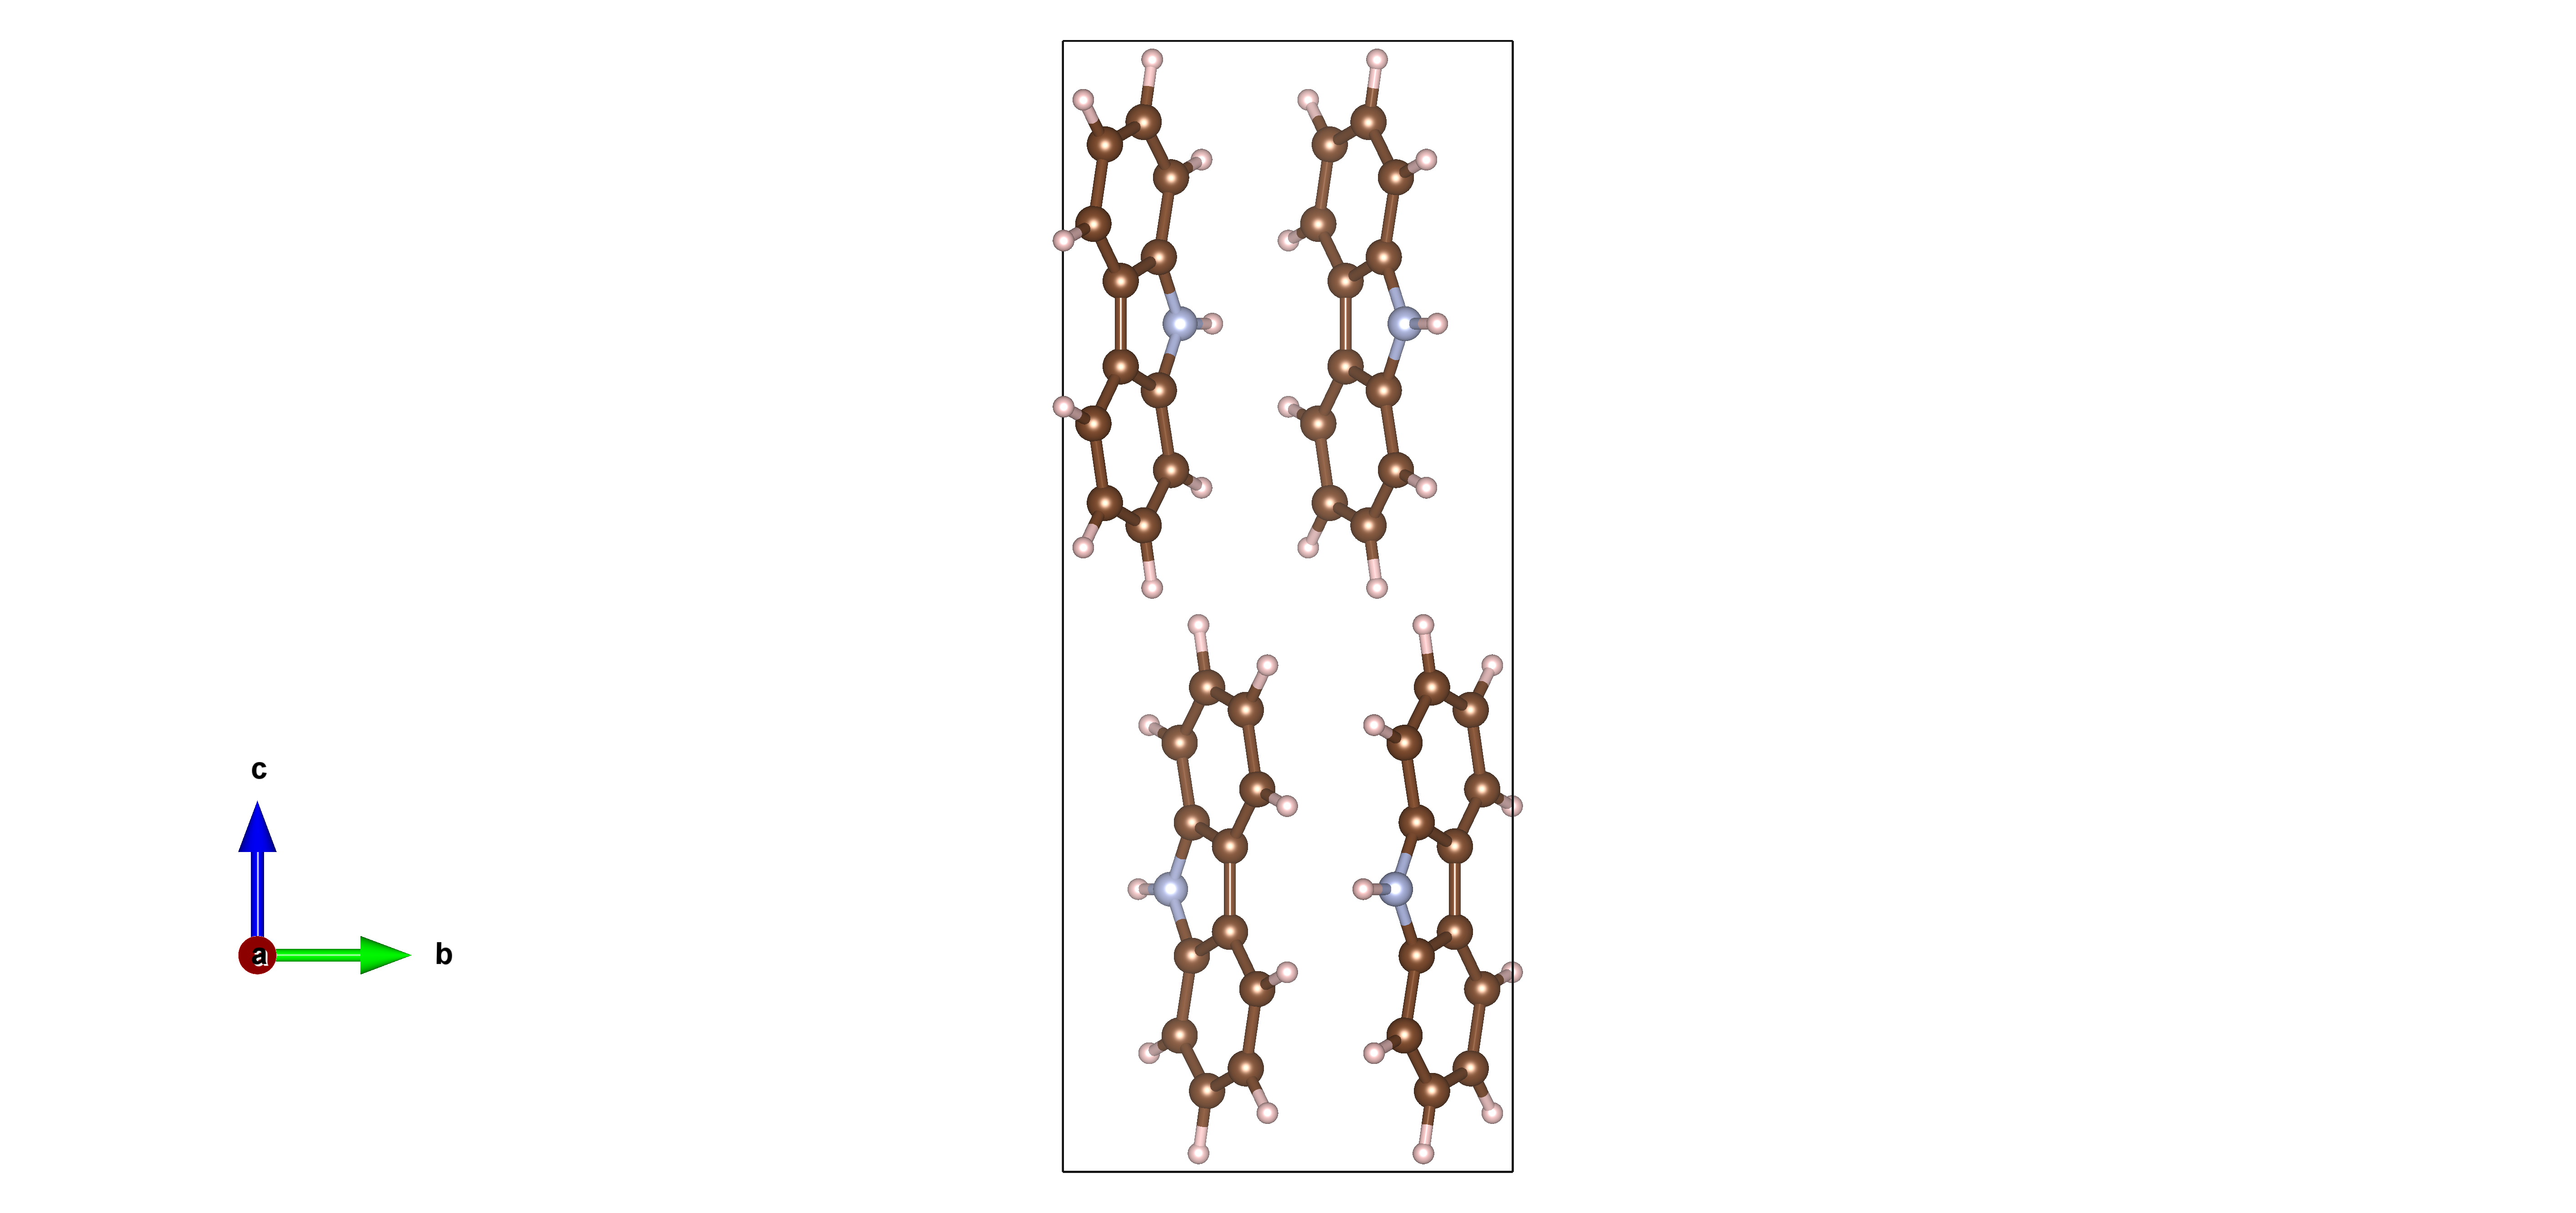
\includegraphics[scale=0.5]{image/Carbazole-a} & 
 		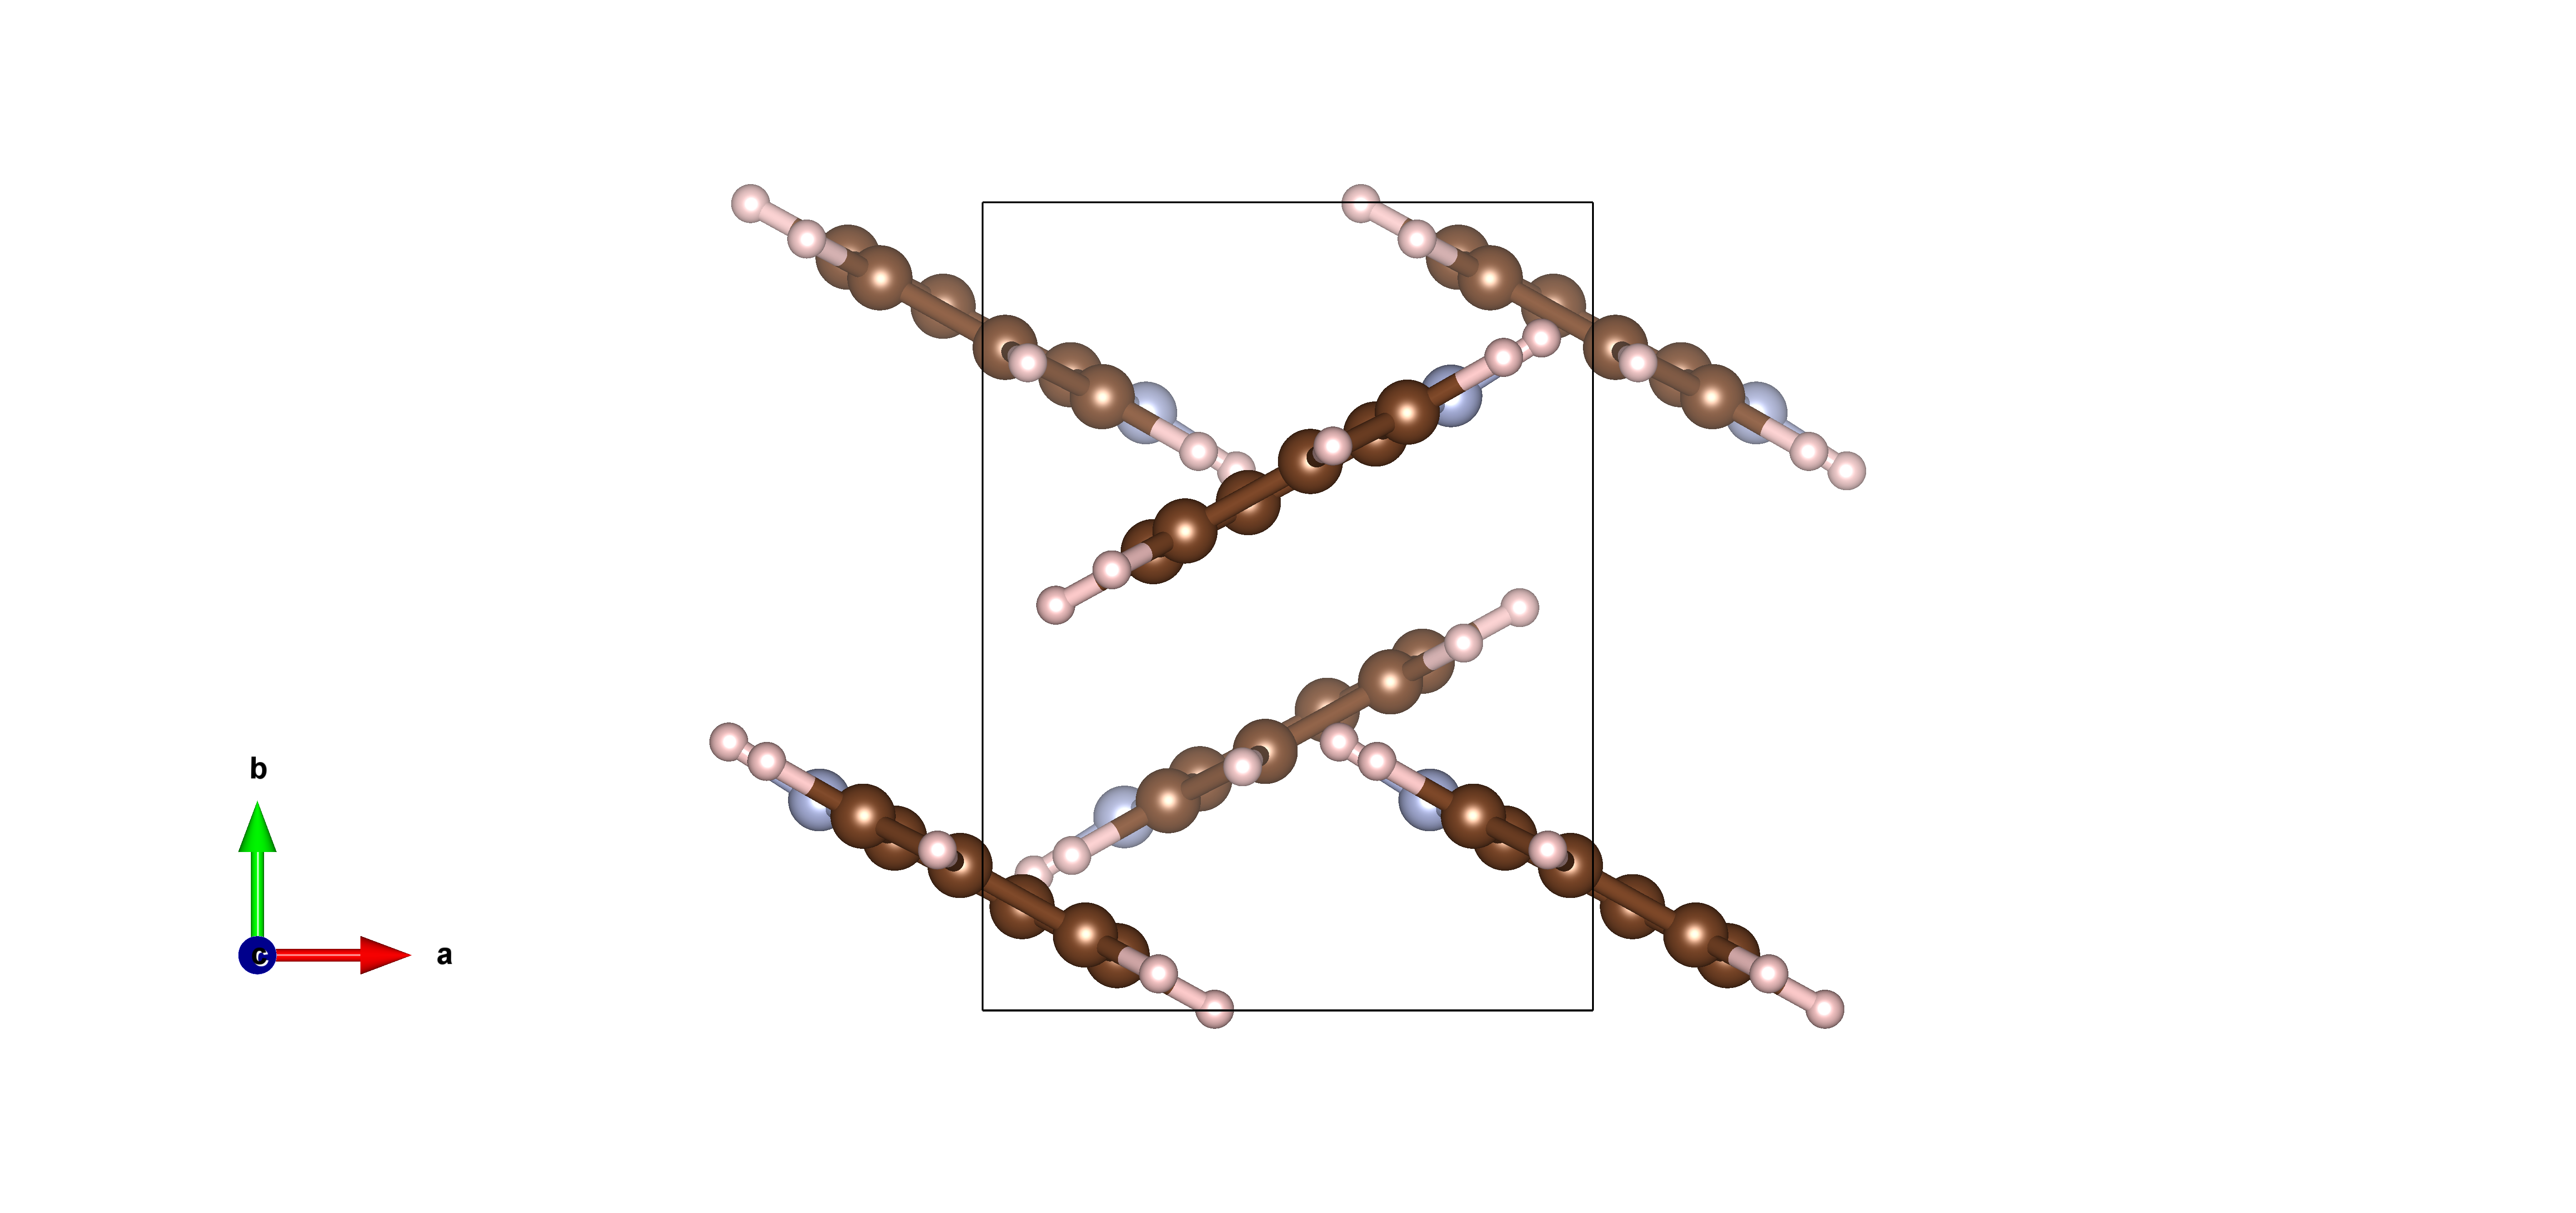
\includegraphics[scale=0.5]{image/Carbazole-c}	 \\
 			\end{tabular}}
 		\caption{The \textit{bc} and \textit{ab} planes of Carbazole crystal}  \label{fig-carbazolesol}
 		\end{center}
 	\end{figure}
 
 	
 		\begin{table}[H]
 			\caption{Lattice parameters of Carbazole molecule calculated in VASP code}  \label{table-carbazolesol}
 			\begin{center}
 				\begin{threeparttable}
 					\begin{tabular}{c c c c c c c}
 						\toprule
 						& \textbf{D2} & \textbf{D3} & \textbf{TS} & \textbf{TS-SCS} & \textbf{PBE*} & \textbf{Exp} ref\cite{belskii1985structure} \\
 						\midrule
 						\textbf{a} & 5.59 (5.51) & 5.77 & 5.70 & 5.70 & 6.07 & 5.71 \\
 						\textbf{b}& 7.27 (7.21) & 7.64 & 7.39 & 7.44 & 8.67 & 7.78\\
 						\textbf{c}& 18.75 (18.86) & 19.20 & 19.08 & 19.07 & 19.67 & 19.11\\
 						\textbf{Volume ($\AA^{3}$)}& 762.34 (749.46) & 846.60 & 804.18 & 808.71 & 1035.61 & 848.88\\
 						\bottomrule
 					\end{tabular}
 					
 					\begin{tablenotes}
 						\item[*] without dispersion correction
 						\item[()] Parenthesis values were calculated with CRYSTAL program
 					\end{tablenotes}
 				\end{threeparttable}
 			\end{center}
 		\end{table}
 
 
 \begin{figure}[H]
 	\begin{center}
 		\resizebox{20cm}{!}{
 			\begin{tabular}{c c}
 			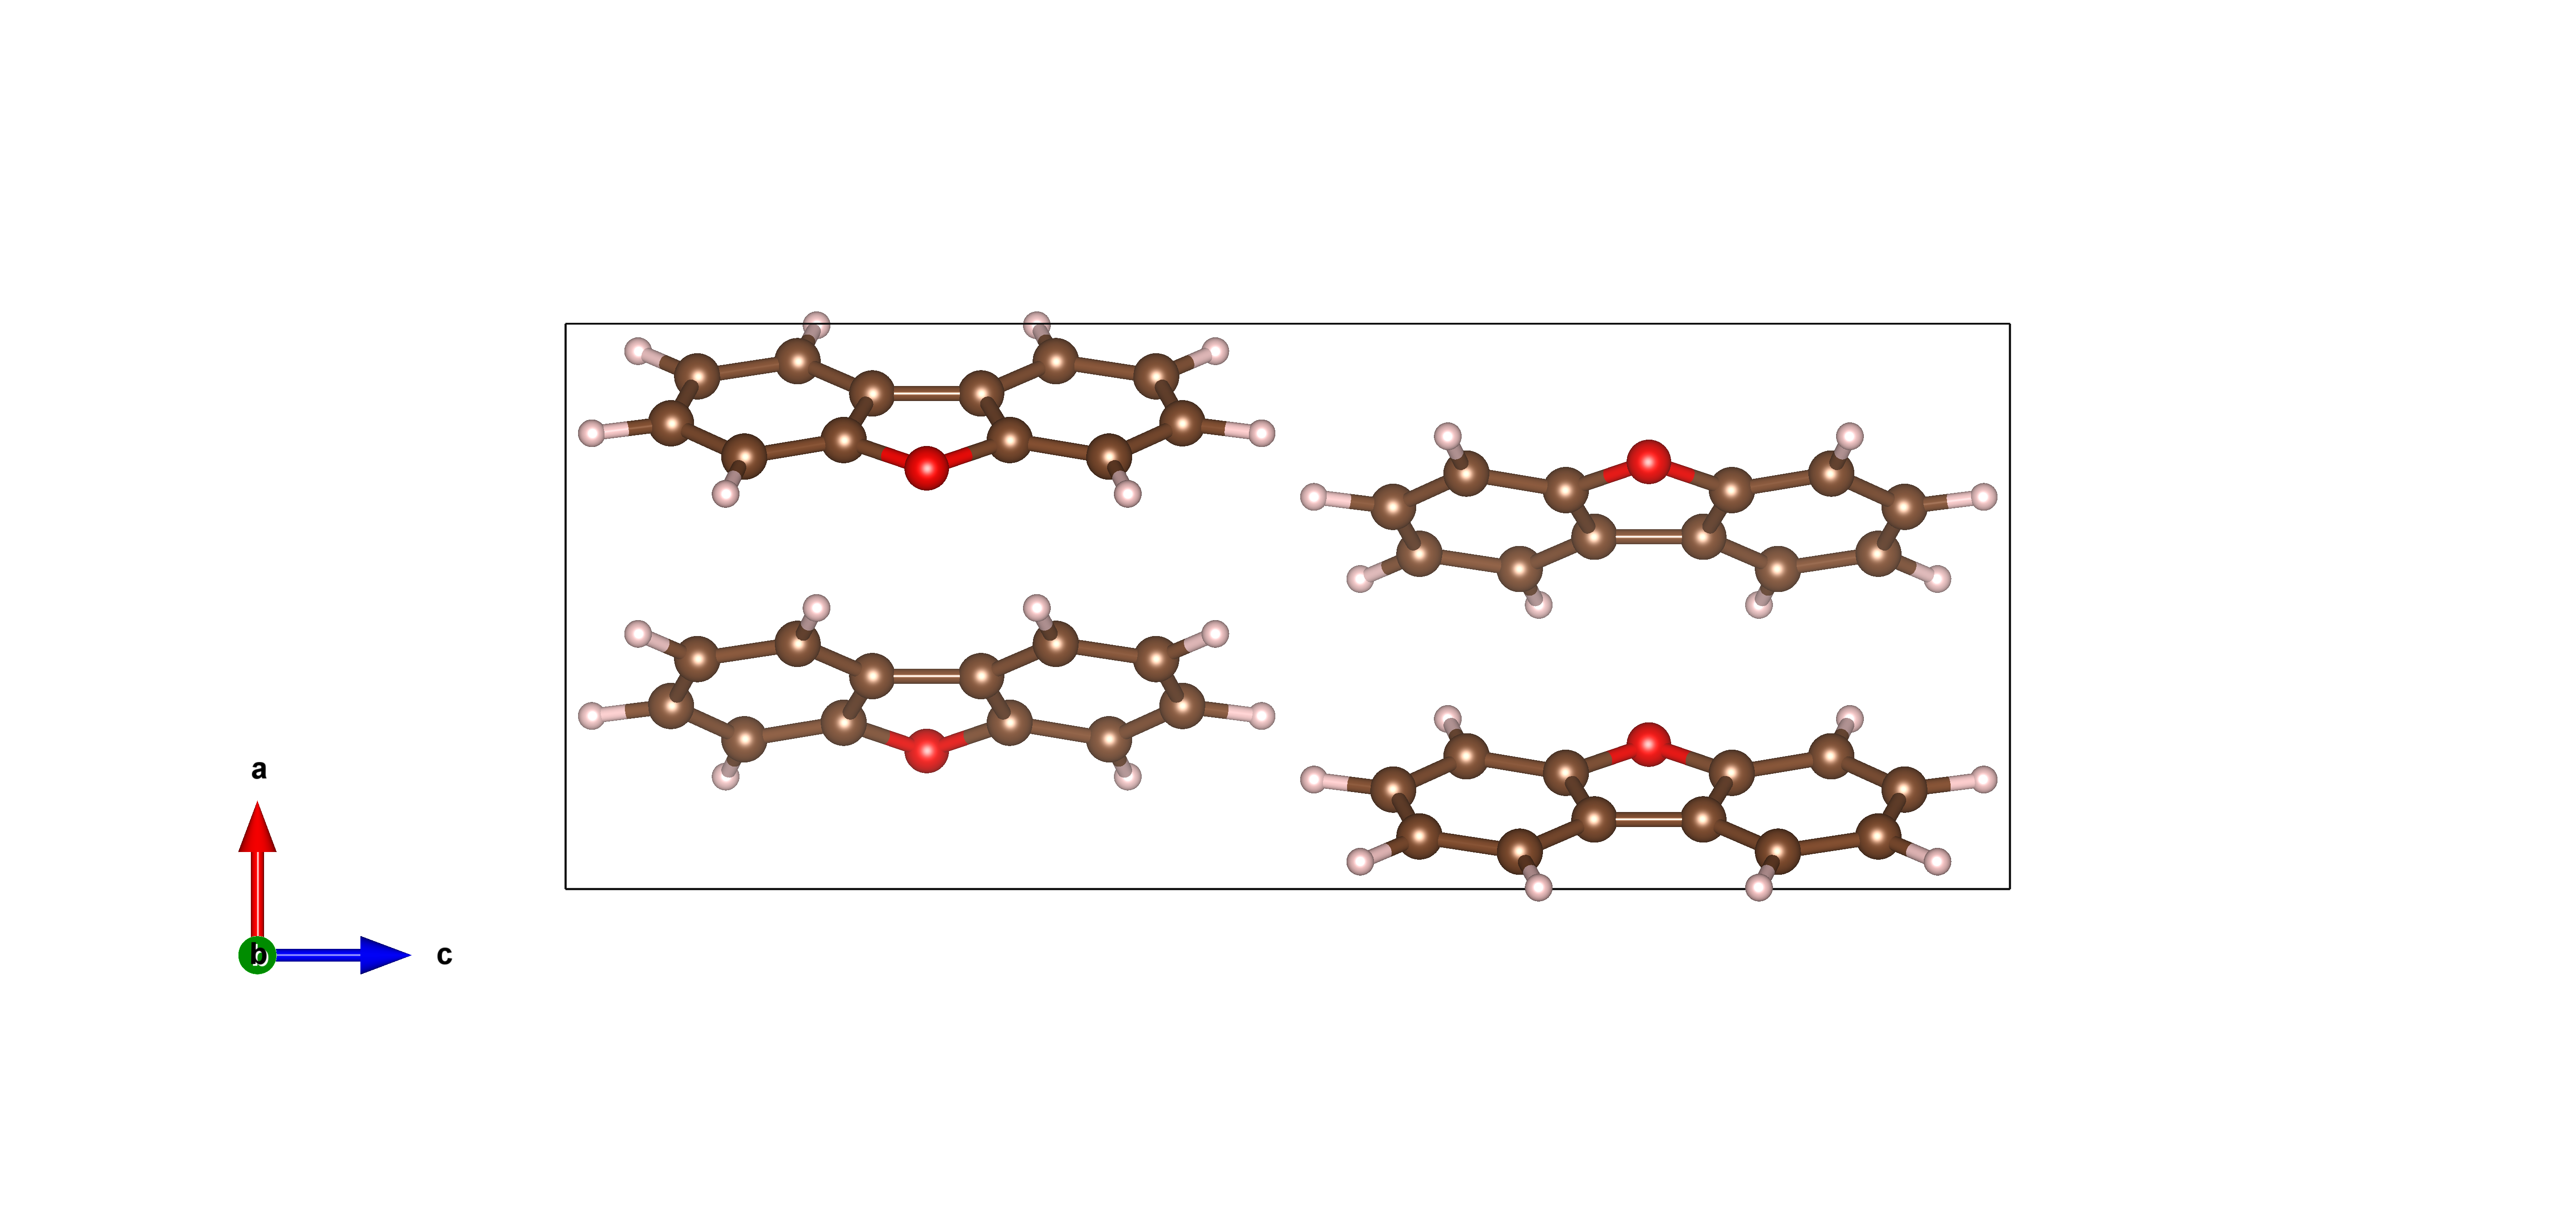
\includegraphics[scale=0.5]{image/Dibenzofuran-b} & 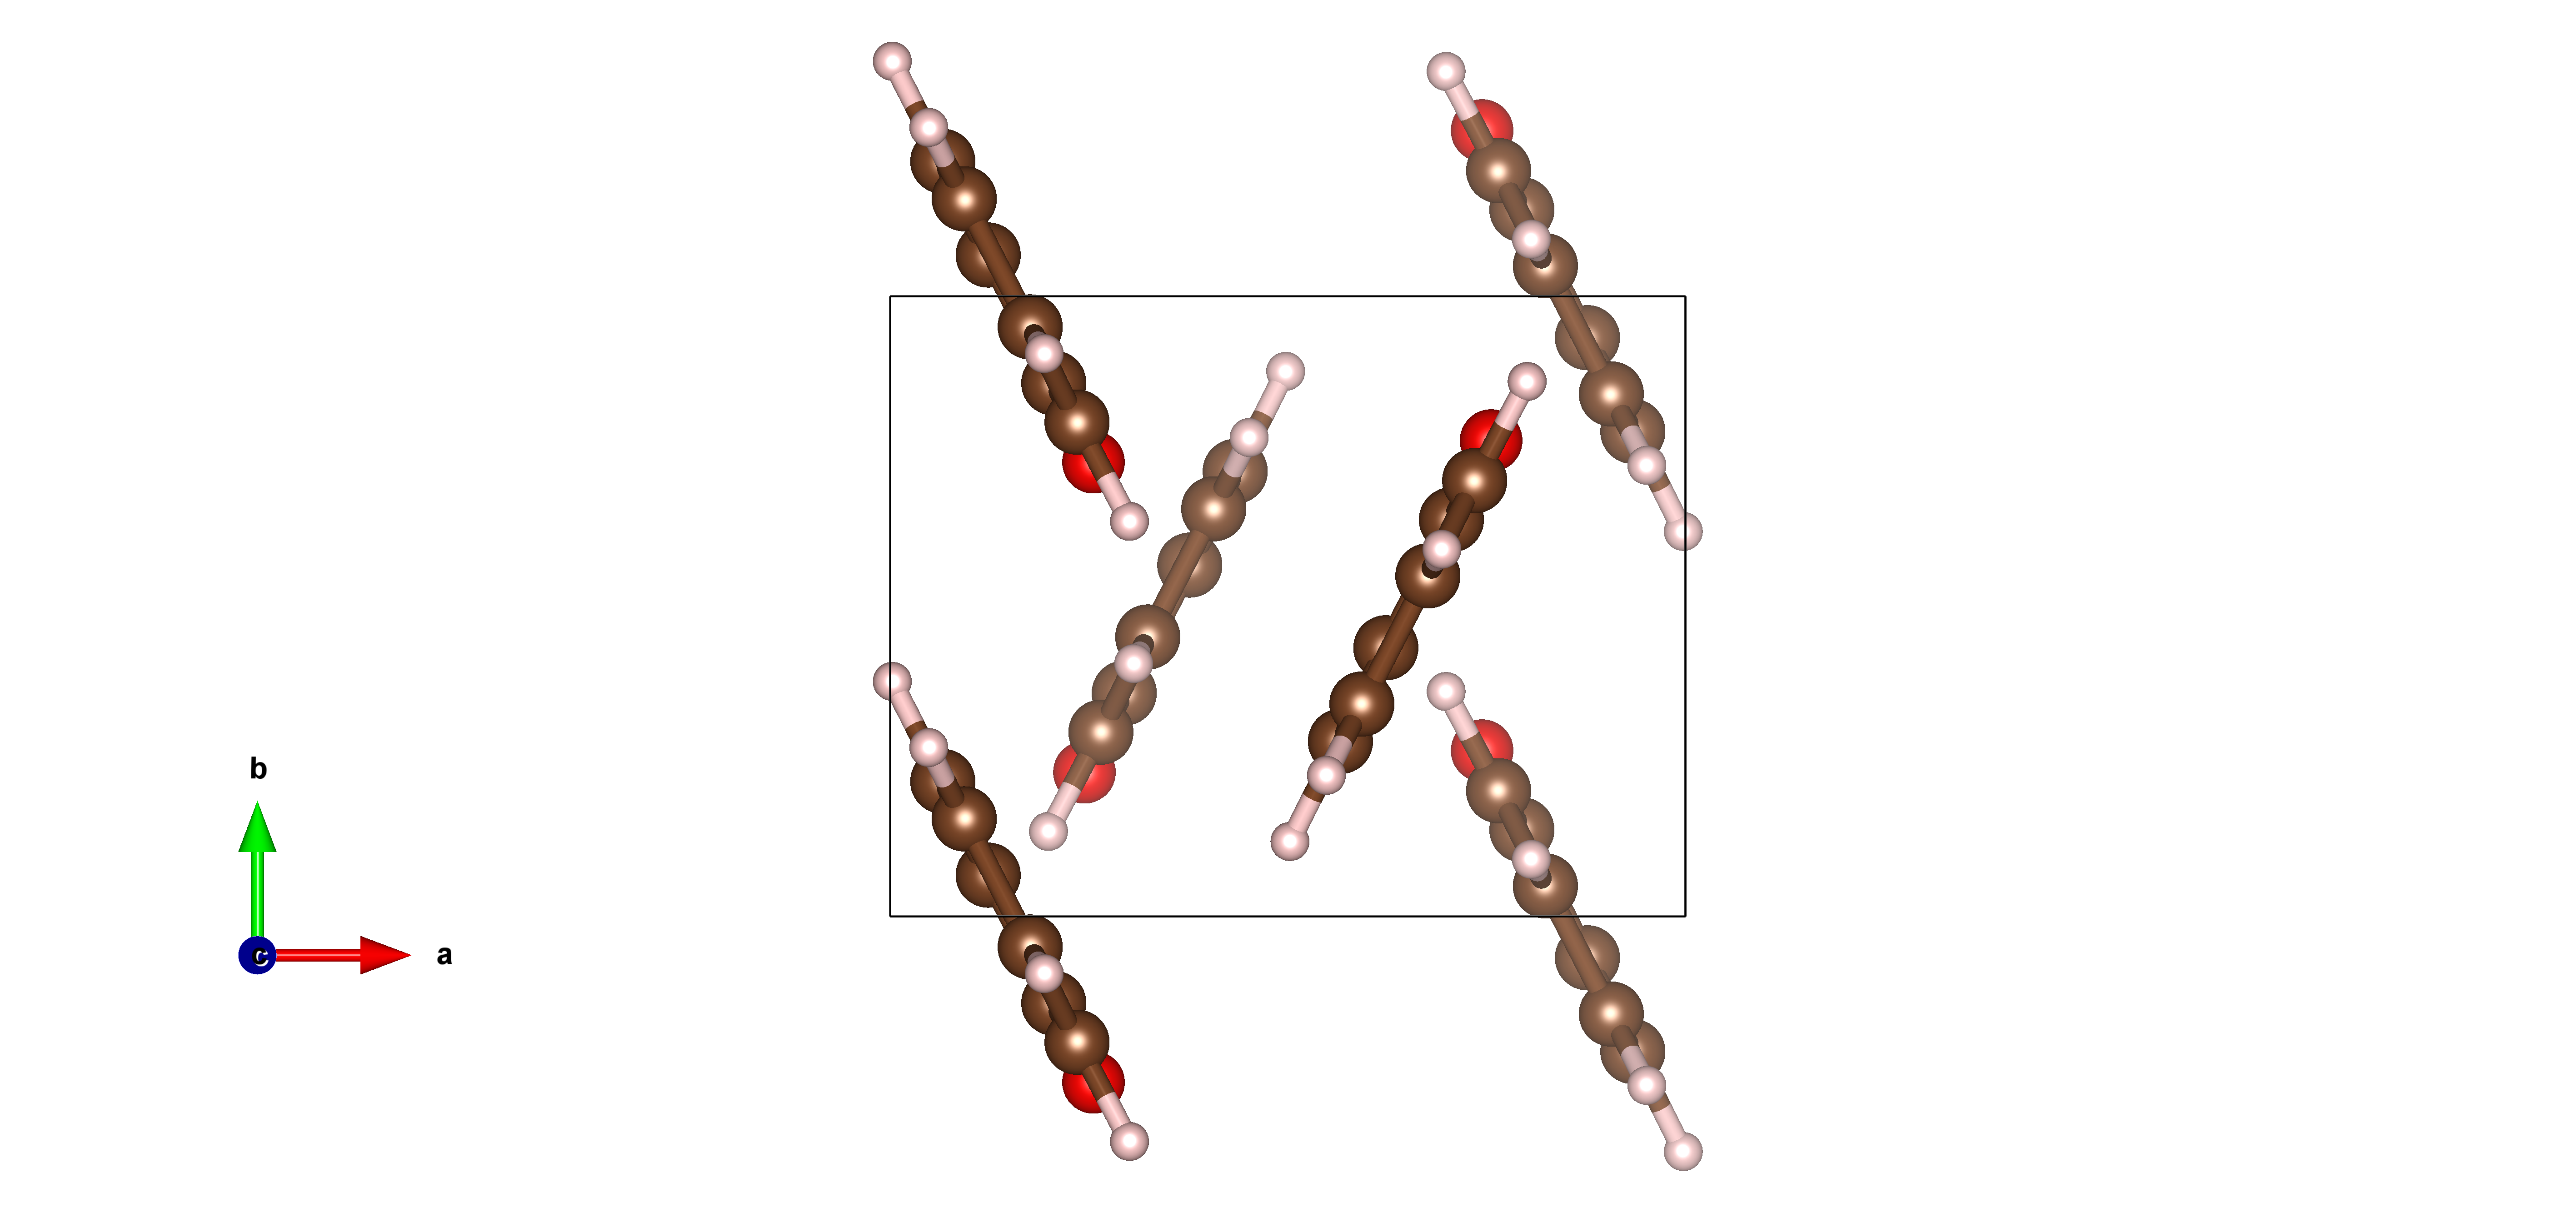
\includegraphics[scale=0.5]{image/Dibenzofuran-c}		 \\
 			\end{tabular}}
 		\caption{The \textit{ac} and \textit{bc} planes of Dibenzofuran crystal}  \label{fig-dibenzofuransol}
 		\end{center}
 	\end{figure}
 	
 	
 	\begin{table}[H]
 	\caption{Lattice parameters of Dibenzofuran molecule calculated in VASP code}  \label{table-dibenzofuransol}
 	\begin{center}
 		\begin{threeparttable}
 			\begin{tabular}{c c c c c c c}
 				\toprule
 				& \textbf{D2} & \textbf{D3} & \textbf{TS} & \textbf{TS-SCS} & \textbf{PBE*} & \textbf{Exp} ref\cite{dideberg1972crystal} \\
 				\midrule
 				\textbf{a} & 7.17 (6.94) & 7.52 & 7.36 &7.34 & 8.68 & 7.70 \\
 				\textbf{b}& 5.69 (5.65) & 5.86& 5.78 & 5.79 & 6.29 & 5.83\\
 				\textbf{c}& 18.84 (20.26) & 19.22 & 19.05 & 19.08 & 19.81 & 19.19\\
 				\textbf{Volume ($\AA^{3}$)}& 769.27 (793.69) & 847.16 & 810.05 & 810.10 & 1082.30 & 860.72\\
 				\bottomrule
 			\end{tabular}
 			
 				\begin{tablenotes}
 					\item[*] without dispersion correction
 					\item[()] Parenthesis values were calculated with CRYSTAL program
 				\end{tablenotes}
 			\end{threeparttable}
 		\end{center}
 	\end{table}
 	
 	
 	\begin{figure}[H]
 		\begin{center}
 			\resizebox{20cm}{!}{
 				\begin{tabular}{c c}
 				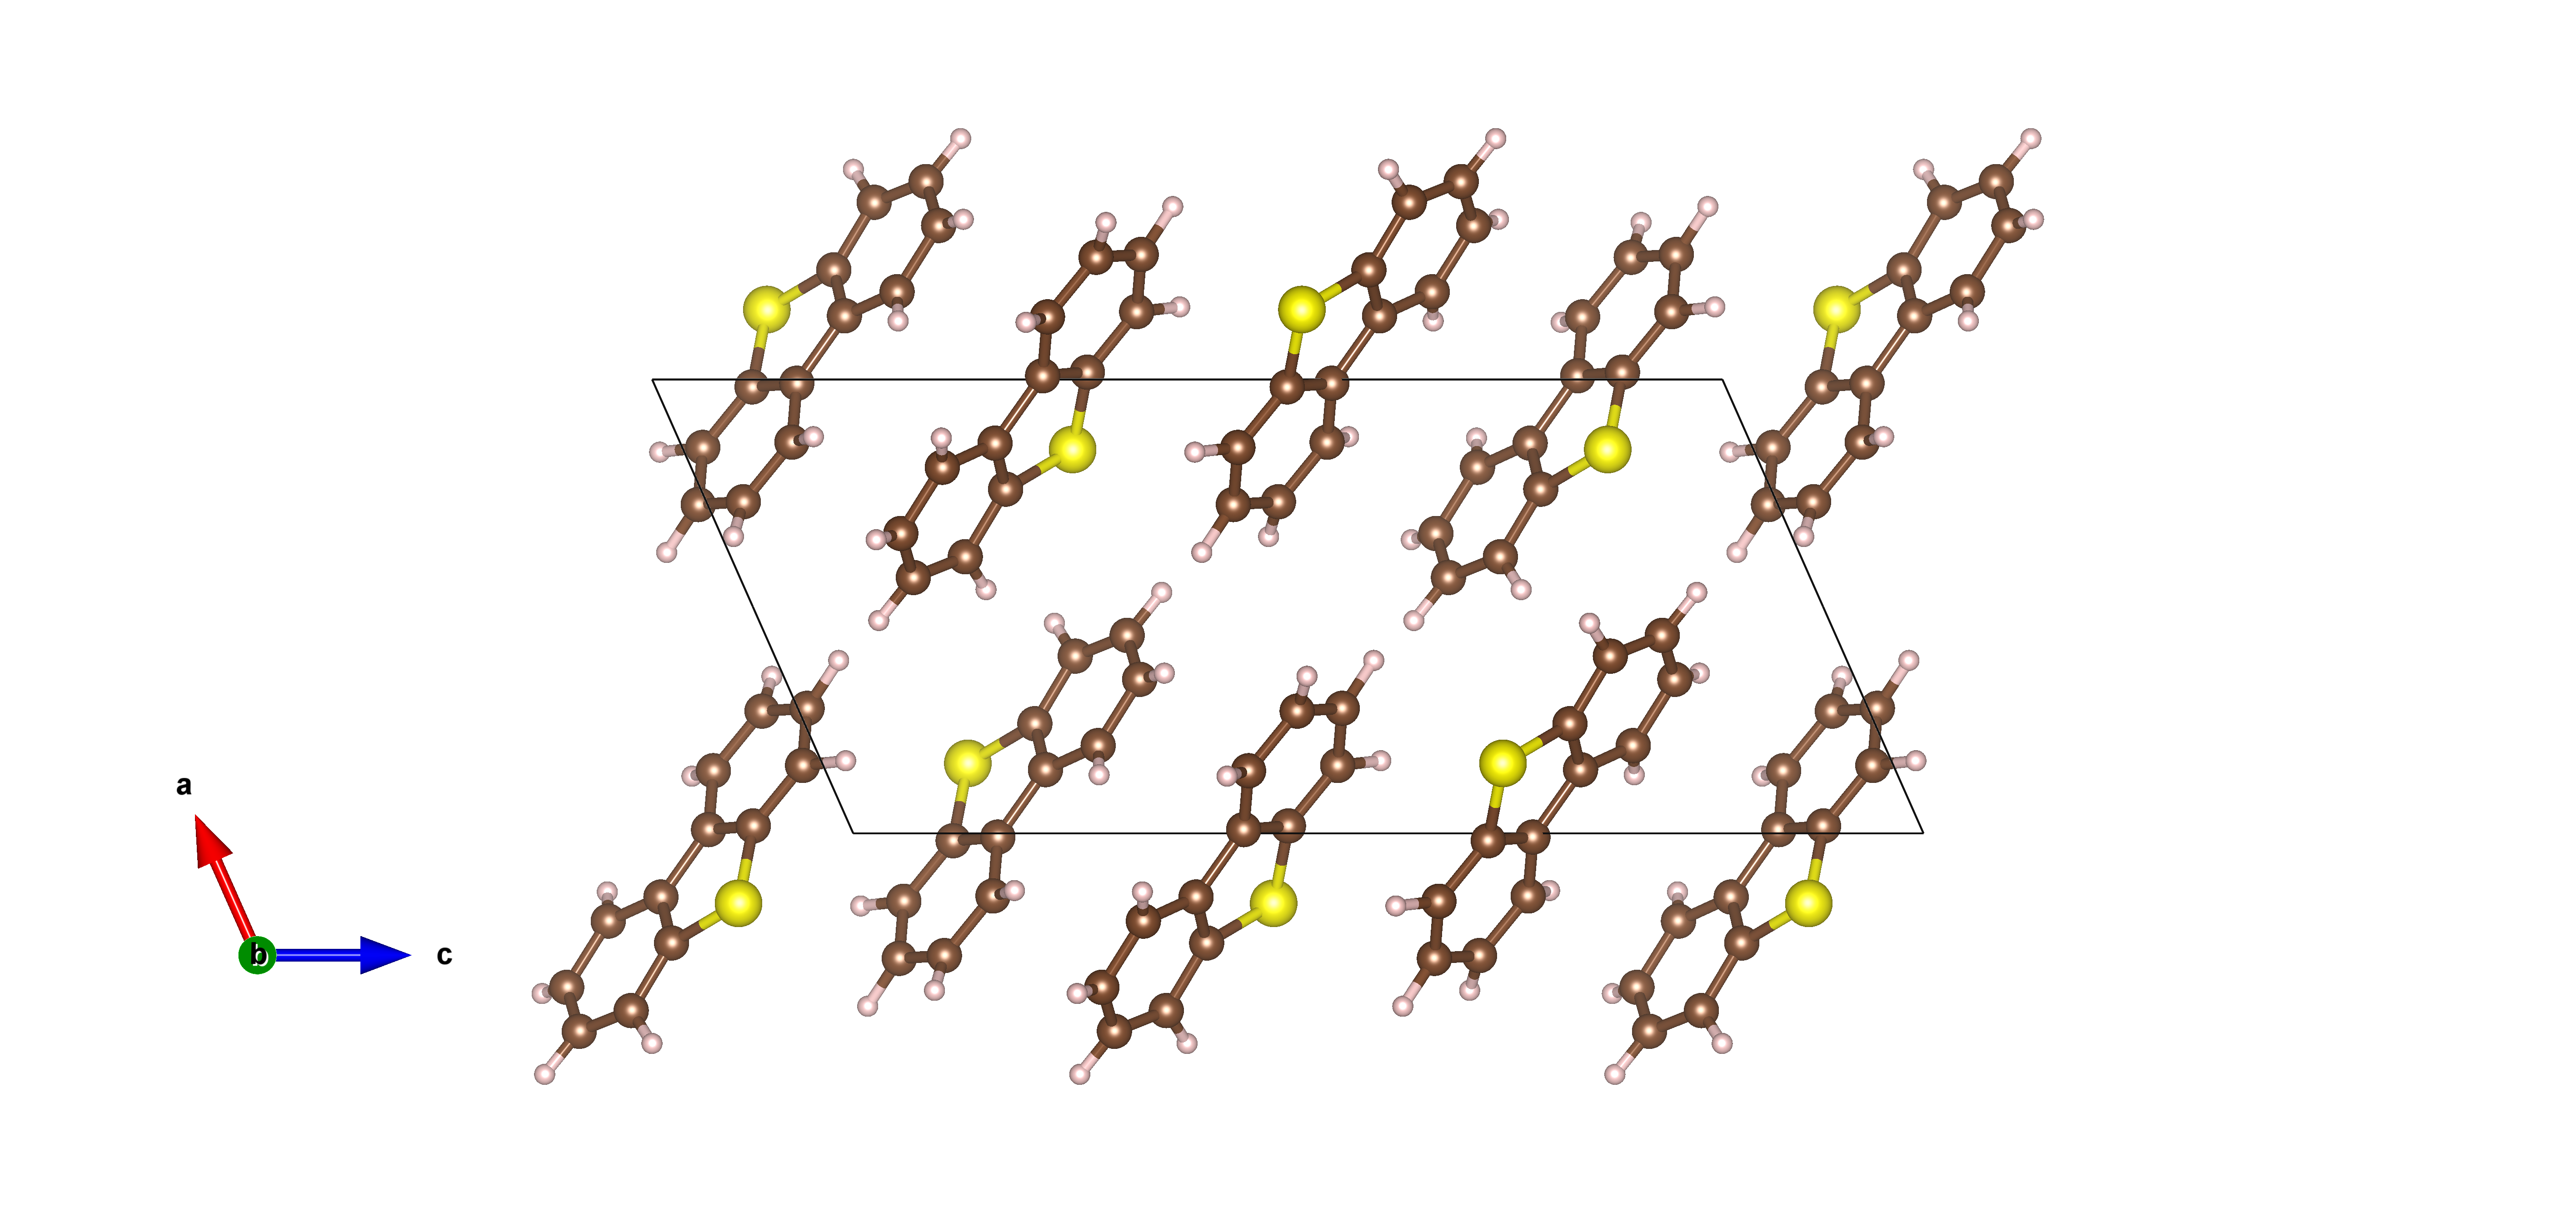
\includegraphics[scale=0.5]{image/Dibenzothiophene-b} & 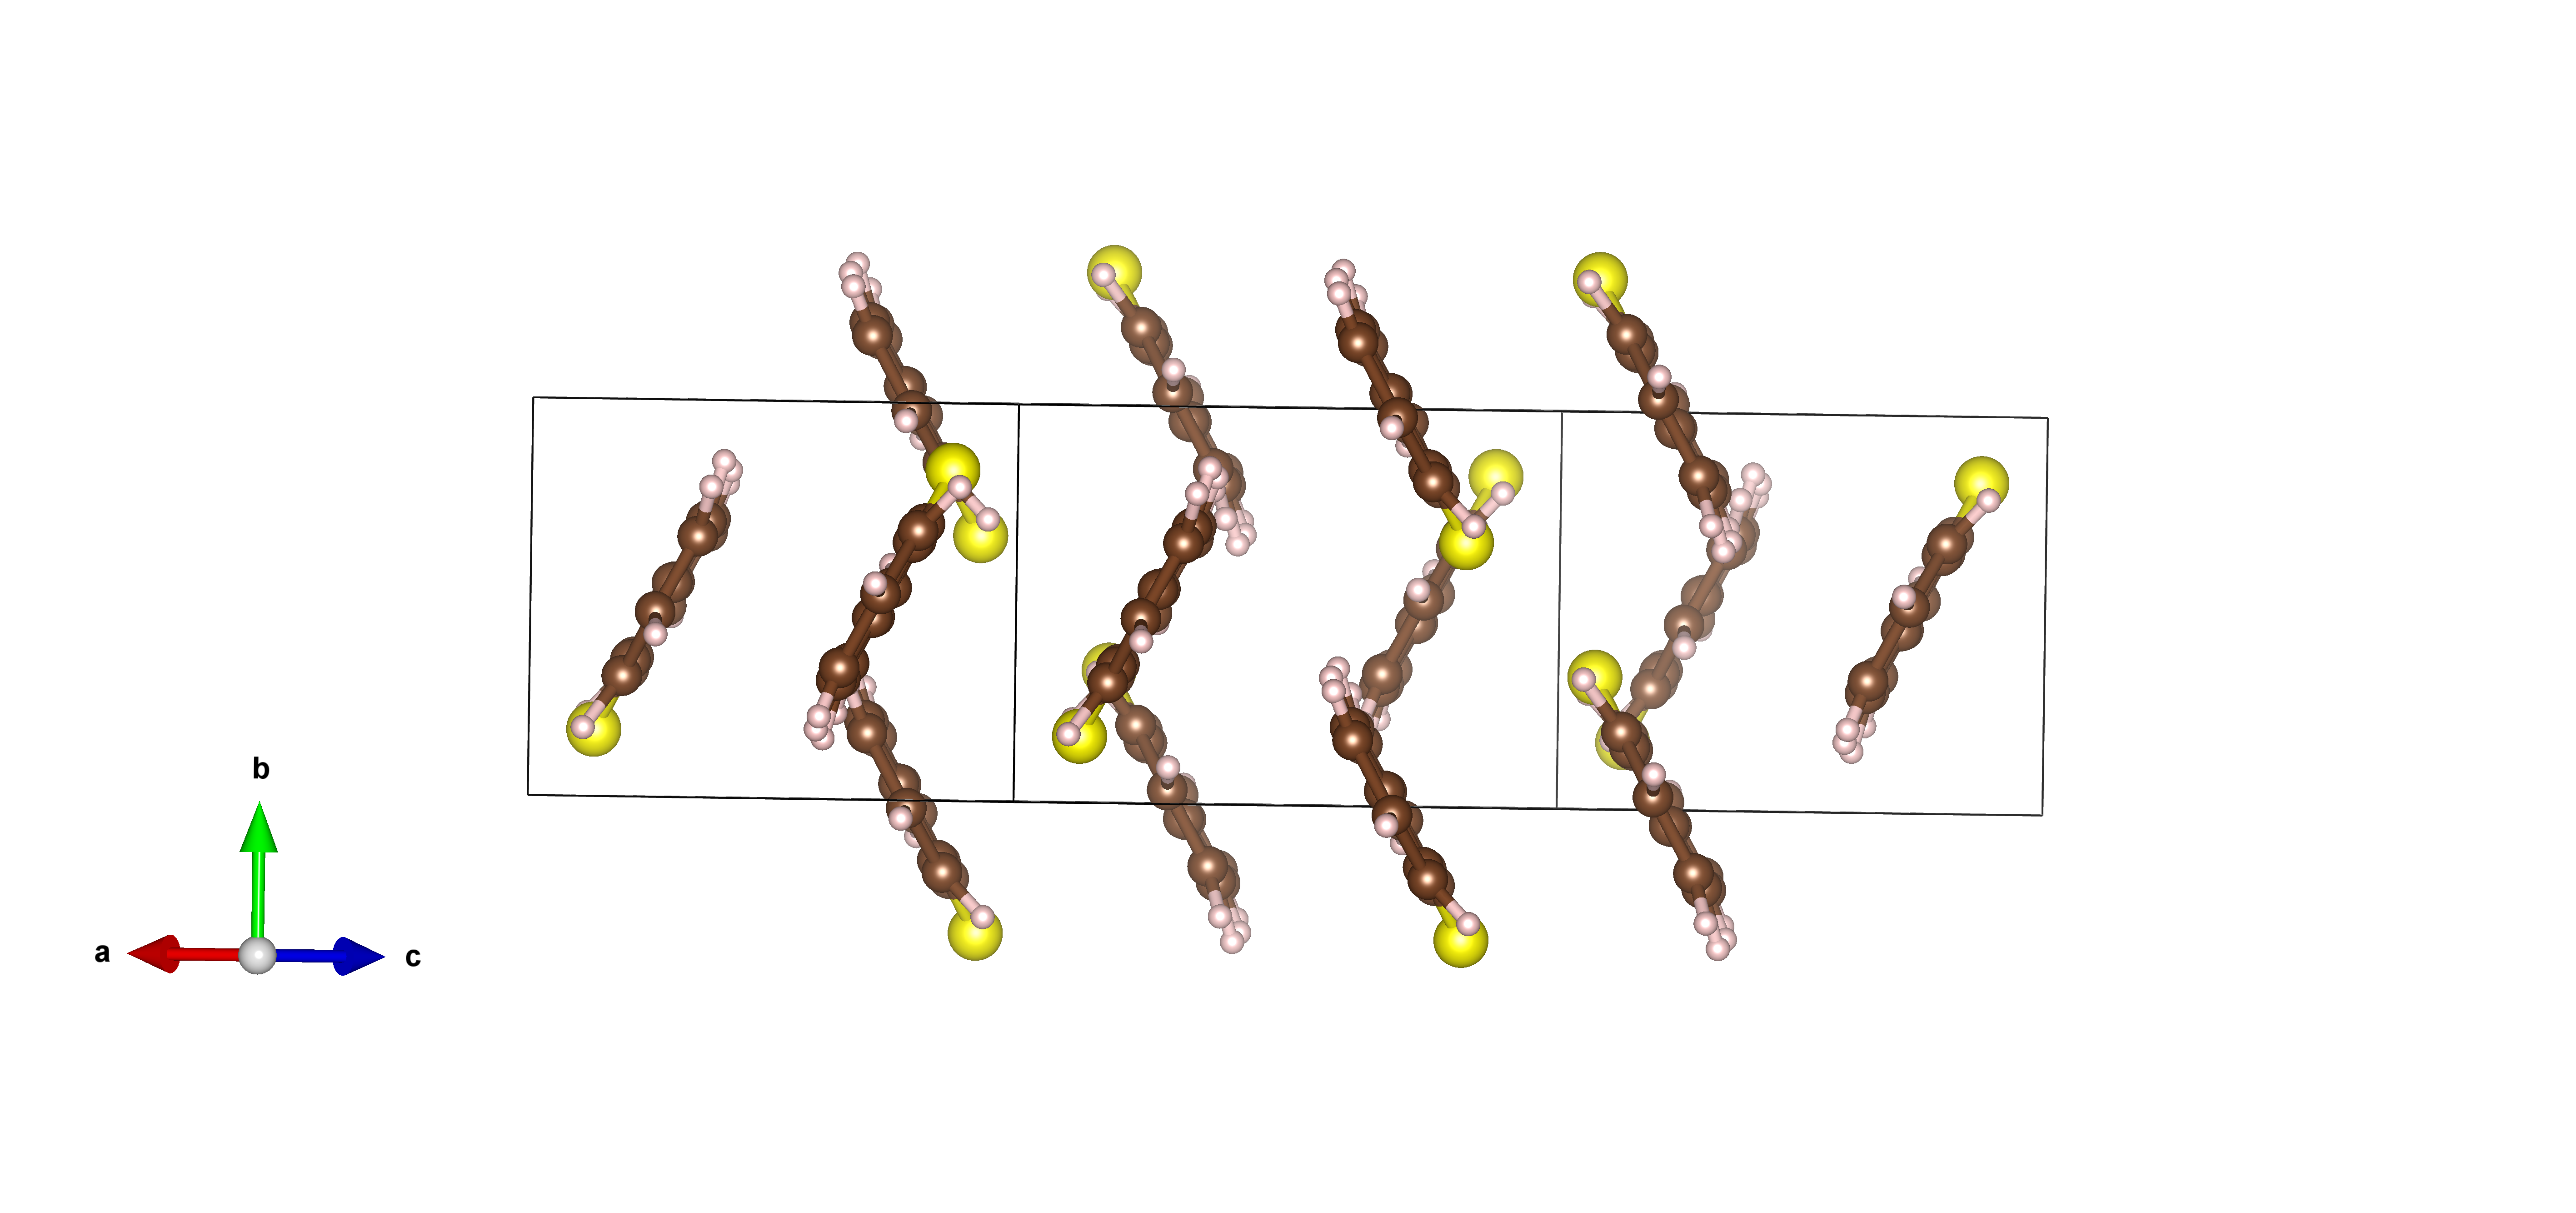
\includegraphics[scale=0.5]{image/Dibenzothiophene-z}		 \\
 				\end{tabular}}
 			\caption{The \textit{ac} plane and other view of molecular arrangement of Dibenzothiophene crystal}  \label{fig-dibenzothiophenesol}	
 			\end{center}
 		\end{figure}
 	
 	
 
 	
 	\begin{table}[H]
 		\caption{Lattice parameters of Dibenzothiophene molecule calculated in VASP code} \label{table-dibenzothiophenesol}
 		\begin{center}
 			\begin{threeparttable}
 				\begin{tabular}{c c c c c c c}
 					\toprule
 					& \textbf{D2} & \textbf{D3} & \textbf{TS} & \textbf{TS-SCS} & \textbf{PBE*} & \textbf{Exp} ref\cite{schaffrin1970structure}\\
 					\midrule
 					\textbf{a} &  8.26 (8.59) & 8.56 & 8.36 & 8.54 & 9.83 & 8.67\\
 					\textbf{b}&5.86 (5.68)  & 6.03 & 5.95 & 6.05 & 6.48 & 6.00\\
 					\textbf{c}& 17.94 (17.83) & 18.44 & 18.04 & 18.39 & 20.95 & 18.70\\
 					\textbf{$\beta$} & 111.54 (112.66) & 112.07 & 111.87& 111.79& 119.32 & 113.90 \\
 					\textbf{Volume ($\AA^{3}$)}&808.18 (802.53) &882.92 &847.06  & 883.16 & 1163.07 & 889.36\\
 					\bottomrule
 				\end{tabular}
 				
 				\begin{tablenotes}
 					\item[*] without dispersion correction
 					\item[()] Parenthesis values were calculated with CRYSTAL program
 				\end{tablenotes}
 			\end{threeparttable}
 		\end{center}
 	\end{table}
 

 	
 		\begin{table}[H]
 			\caption{ Calculated vibrational frequencies (cm$^{-1}$) of the monomer, dimer and solid-state (PBE Carbazole system).}  \label{table-freqCarbaz}
 			\begin{center}
 				\begin{threeparttable}
 					\resizebox{17cm}{!}{
 					\begin{tabular}{c c c c c}
 						\toprule
 						\multicolumn{2}{p{4.5cm}}{\centering \textbf{Monomer}} & \textbf{Dimer} & \multicolumn{1}{p{4cm}}{\centering \textbf{Experimental} \\ Fig} & \textbf{VASP/CRYSTAL}\\
 						Assignment & $\nu$(cm$^{-1}$) & $\nu$(cm$^{-1}$) & $\nu$(cm$^{-1}$) & $\omega$(cm$^{-1}$) \\
 						& Int(km/mol) & Int(km/mol) & & Int(km/mol) \\
 						\midrule
 						&  &  \textit{26 (0.05)}& & \\
 						&  & \textit{31 (0.03)} &  & \\
 						&  & \textit{43 (0.02)}&  & \\
 						& & \textit{65 (1.32)} &\multirow{2}{2cm}{\centering 71 (w)}  & \textit{66 (0.13)}\\
 						&  & \textit{70 (0.01)}&  & \textit{72 (13.88)} \\
 						&  & \textit{95 (0.51)} &  &\\
 						\\
 						\multirow{3}{3cm}{\centering $\nu_{1}$}& \multirow{3}{3cm}{\centering 103 (5.54)} & \multirow{3}{3cm}{\centering 115 (2.85) \\ 158 (0.11)} & \multirow{3}{3cm}{\centering 125 (m)}  & 112 (0.86) \\
 						&   &   &  & \textit{114 (3.31)}\\
 						&  &  &   & \textit{118 (26.62)}\\
 						\multirow{2}{2cm}{\centering $\nu_{2}$}& \multirow{2}{2cm}{\centering 150 (0.00)} &  153 (0.12) & \multirow{2}{2cm}{\centering 146 (w) } & \multirow{2}{2cm}{\centering 142 (8.41)}\\
 						&   & 168 (0.04)  &   & \\ 
 						&  &  & 190 (vw) & 185 (0.49)\\
 						\multirow{2}{2cm}{\centering $\nu_{3}$}& \multirow{2}{2cm}{\centering 222 (0.38)}& 221 (0.47) & \multirow{2}{2cm}{\centering 221 (m)}& 221 (0.26)\\
 						 &  &  221 (0.35) &  & 222 (0.52)\\
 						 \multirow{2}{2cm}{\centering $\nu_{4}$}& \multirow{2}{2cm}{\centering 284(15.47)} & 301 (0.74) & \multirow{2}{2cm}{\centering 294 (w)} & \multirow{2}{2cm}{\centering 283 (0.43)}\\
 						 &   & 305 (0.01) &  & \\ 
 						  \multirow{2}{2cm}{\centering $\nu_{5}$}& \multirow{2}{2cm}{\centering 297 (0.00)} & 321 (0.02) &  \multirow{2}{2cm}{\centering 312 (w)} & 303 (9.96)\\
 						  & & 325 (2.83) &  & 309 (12.45)\\
 						 $\nu_{6}$& 344(61.71) &   &   & \\
 						  \multirow{2}{2cm}{\centering $\nu_{7}$}& \multirow{2}{2cm}{\centering 434(11.32)} & 431 (7.50) &  \multirow{4}{4cm}{\centering 423 (s)} & 418 (63.87)\\
 						  &   &  438 (11.67) &  & 419 (6.27)\\
 						\multirow{2}{2cm}{\centering $\nu_{8}$}& \multirow{2}{2cm}{\centering 439 (1.44)} & 435 (5.64) &   &  \multirow{2}{2cm}{\centering 428 (0.78)}\\
 						&   & 436 (77.40) &    &  \\
 						&   &  446 (203.89) &  \multirow{4}{4cm}{\centering 445 (s)}&  \multirow{2}{2cm}{\centering 434(43.81)} \\
 						&   &  447 (30.18) &   & \\
 						 \multirow{2}{2cm}{\centering $\nu_{5}$}& \multirow{2}{2cm}{\centering 453 (0.00)} & 457 (13.23) &    &  \multirow{2}{2cm}{\centering 441 (1.34)} \\
 						 &   &  458 (0.02) &    &  \\
 						\bottomrule	    
 					\end{tabular}}
 					
 					\begin{tablenotes}
 						\item[] Italic: Intermolecular modes
 					\end{tablenotes}
 				\end{threeparttable}
 			\end{center}
 		\end{table}	
 	
 	
 	    \begin{spacing}{1.1}
 		\begin{table}[H]
 			\caption{ Calculated vibrational frequencies (cm$^{-1}$) of the monomer, dimer and solid-state (PBE Dibenzofuran system).}  \label{table-freqDibenzof}
 			\begin{center}
 				\begin{threeparttable}
 					\resizebox{17cm}{!}{
 					\begin{tabular}{c c c c c}
 						\toprule
 						\multicolumn{2}{p{4.5cm}}{\centering \textbf{Monomer}} & \textbf{Dimer} & \multicolumn{1}{p{4cm}}{\centering \textbf{Experimental} \\ ref \cite{klots1996vibrational}} & \textbf{VASP/CRYSTAL}\\
 						Assignment & $\nu$(cm$^{-1}$) & $\nu$(cm$^{-1}$) & $\nu$(cm$^{-1}$) & $\omega$(cm$^{-1}$) \\
 						& Int(km/mol) & Int(km/mol) & & Int(km/mol) \\
 						\midrule
 						&  &  \textit{12 (0.03)}& & \\
 						&  & \textit{27 (0.04)} &  & \\
 						&  & \textit{37 (0.09)}&  & \\
 						& & \textit{63 (0.06)} &  & \textit{53 (1.83)}\\
 						&  & \textit{78 (0.26)}&  & \textit{78 (0.01)} \\
 						&  & \textit{88 (0.08)} &  &  \\
 						\\
 						\multirow{3}{3cm}{\centering $\nu_{1}$}& \multirow{3}{3cm}{\centering 105 (2.18)} & \multirow{3}{3cm}{\centering 121 (4.03) \\ 126 (0.04)} & \multirow{3}{3cm}{\centering 103}  & \textit{106 (3.86)}\\
 						 &   &   &   &  \textit{108 (0.75)}\\
 						 &   &   &    & 117 (1.09)\\
                        \multirow{2}{2cm}{\centering $\nu_{2}$}& \multirow{2}{2cm}{\centering 152 (0.00)} & 163 (0.04) & \multirow{2}{2cm}{\centering 150} & 140 (0.47)\\
                        &   &  167 (0.06)&   & 152 (0.14)\\
                        \multirow{2}{2cm}{\centering $\nu_{3}$}& \multirow{2}{2cm}{\centering 222 (1.19)} & 222 (0.34) & \multirow{2}{2cm}{\centering 217} & 217 (0.42)\\
                        &   &   222 (1.52) &   & 221 (2.86)\\ 						
 						\multirow{2}{2cm}{\centering $\nu_{4}$}& \multirow{2}{2cm}{\centering 294 (0.00)} & 299 (0.05) & \multirow{2}{2cm}{\centering 287}& \multirow{2}{2cm}{\centering 286 (0.01)}\\
 					  &   &  302 (0.11) &  &  \\
 					  \multirow{2}{2cm}{\centering $\nu_{5}$}& \multirow{2}{2cm}{\centering 317 (0.01)} & 321 (0.28) & \multirow{2}{2cm}{\centering 310} & 314 (0.22)\\
 					  &   &  323 (0.02) &  &  317 (1.27)\\
 					  \multirow{2}{2cm}{\centering $\nu_{6}$}& \multirow{2}{2cm}{\centering 434 (6.24)} & 434 (10.51) & \multirow{2}{2cm}{\centering 419} & 413 (1.65)\\
 					  &   &  437 (2.71) &  & 434 (26.52)\\
 					  \multirow{2}{2cm}{\centering $\nu_{7}$}& \multirow{2}{2cm}{\centering 434 (1.88)} & 436 (1.41) & \multirow{2}{2cm}{\centering 424}& \multirow{2}{2cm}{\centering 425 (6.91)}\\
 					  &   &  436 (1.47) &  &  \\
 						\bottomrule	    
 					\end{tabular}}
 					
 					\begin{tablenotes}
 						\item[] Italic: Intermolecular modes
 					\end{tablenotes}
 				\end{threeparttable}
 			\end{center}
 		\end{table}
 	\end{spacing}
 
 
 
 
 	\begin{table}[H]
 		\caption{ Calculated vibrational frequencies (cm$^{-1}$) of the monomer, dimer and solid-state (PBE Dibenzothiophene system).}  \label{table-freqDibenzothio}
 		\begin{center}
 			\begin{threeparttable}
 				\resizebox{17cm}{!}{
 				\begin{tabular}{c c c c c}
 					\toprule
 					\multicolumn{2}{p{4.5cm}}{\centering \textbf{Monomer}} & \textbf{Dimer} & \multicolumn{1}{p{4cm}}{\centering \textbf{Experimental} \\ Table } & \textbf{VASP/CRYSTAL}\\
 					Assignment & $\nu$(cm$^{-1}$) & $\nu$(cm$^{-1}$) & $\nu$(cm$^{-1}$) & $\omega$(cm$^{-1}$) \\
 					& Int(km/mol) & Int(km/mol) & & Int(km/mol) \\
 					\midrule
 					&  &  \textit{18 (0.05)}& & \\
 					&  & \textit{28 (0.01)} &  & \\
 					&  & \textit{36 (0.09)}&  & \textit{49 (0.38)}\\
 					& & \textit{70 (0.32)} &  & \textit{80 (1.86)} \\
 					&  & \textit{89 (0.01)}&  & \textit{84 (0.07)} \\
 					&  & \multirow{2}{2cm}{\centering \textit{93 (0.56)}} &  & \textit{91 (2.43)} \\
 						&   &   &   &  \textit{99 (0.47)}\\
 				    &   &   &   & \textit{108 (0.60)}\\
 				    &   &   &  & \textit{113 (2.61)}\\
 					\\
 					\multirow{2}{2cm}{\centering $\nu_{1}$}& \multirow{2}{2cm}{\centering 102 (1.54)} & 118 (2.14) & \multirow{2}{2cm}{\centering 135 (m)}  & 138 (0.03)\\
 					&  &   128 (0.06) &   & 140 (1.14)\\
 					\multirow{2}{2cm}{\centering $\nu_{2}$} & \multirow{2}{2cm}{\centering 135 (0.00)} & 147 (0.04) & & 163 (0.45)\\ 
 					&    &   162 (0.10) &   & 172 (0.39)  \\
 				 \multirow{2}{2cm}{\centering $\nu_{3}$} & \multirow{2}{2cm}{\centering 217 (0.85)} & 217 (0.29) & \multirow{2}{2cm}{\centering 213 (m)} & 213 (2.52) \\
 				 &   &  217 (1.09) &  & 215 (5.04)\\
 				 \multirow{2}{2cm}{\centering $\nu_{4}$} & \multirow{2}{2cm}{\centering 221 (1.46)} & 231 (3.05) & \multirow{2}{2cm}{\centering 228 (m)} & 229 (1.93)\\
 				&   & 235 (0.07) &  & 230 (3.94)\\
 				&   &   &  269 (vw) & \\
 				\multirow{2}{2cm}{\centering $\nu_{5}$} & \multirow{2}{2cm}{\centering 279 (0.00)} & 286 (0.01) & \multirow{2}{2cm}{\centering 282 (vw)} & 278 (0.39)\\
 				&   &  289 (0.13) &  &  283 (0.11)\\
 				\multirow{2}{2cm}{\centering $\nu_{6}$} & \multirow{2}{2cm}{\centering 416 (2.83)} & 416 (0.24) & \multirow{2}{2cm}{\centering 404 (s)} & 404 (8.59)\\
 				&  &  416 (4.21) &  & 406 (0.39)\\
 				\multirow{3}{3cm}{\centering $\nu_{7}$} & \multirow{3}{3cm}{\centering 428 (0.15)} & \multirow{3}{3cm}{\centering 428 (0.24) \\ 429 (0.08)} & \multirow{3}{3cm}{\centering 419 (sh)}	& 415 (6.30)\\
 				&   &   &  & 416 (0.60)\\
 				&  &  &  & 418 (0.24)\\
 				\multirow{2}{2cm}{\centering $\nu_{8}$} & \multirow{2}{2cm}{\centering 433 (7.15)} & 433 (16.66) & \multirow{2}{2cm}{\centering 425 (s)} & 423 (18.48)\\
 				&  &  435 (0.23) &  & 435 (3.29)\\
 				\bottomrule	    
 				\end{tabular}}
 				
 				\begin{tablenotes}
 					\item[] Italic: Intermolecular modes
 				\end{tablenotes}
 			\end{threeparttable}
 		\end{center}
 	\end{table}	
 	
 
\newpage	
 	
%-------------------------------------------------------------------------------------------------------------------------
%-------------------------------------------------------------------------------------------------------------------------
%-------------------------------------------------------------------------------------------------------------------------
\section*{Conclusions}
%-------------------------------------------------------------------------------------------------------------------------
%-------------------------------------------------------------------------------------------------------------------------
%-------------------------------------------------------------------------------------------------------------------------
 
The DFT calculations presented in this work provide detailed and accurate descriptions of experimental photoacoustic far IR spectra for acene familly and for far IR spectra of the various aromatic compounds as a whole. Inter- and intramolecular vibrations are discriminated, and combinations of inter- and intramolecular vibrations are identified specially with the use of solid-state conditions. Peak assignment ambiguity, and the potential impacts of molecular distortion on peak intensity are addressed. By examining computed and experimental spectra for the family of acene molecules concurrently, trends in vibration modes with molecular size were used to reinforce assignments, and to reattribute assignments made previously in the experimental spectra.\\

The intermolecular vibrations for aromatic compounds are found in the same wavelength range of the far infrared spectrum. The specificity of the aromatics $\pi$-stacking interactions, reinforced by calculations with distorted dimers and solid-state calculations, allows not only the identification of this family of molecules, but also highlights the presence of $\pi$-stacking interaction in a mixture as a whole. As illustration, the example of the carbazole is reported in figure \ref{figure666}.\\

 \begin{figure}[H]
 	\centering
 	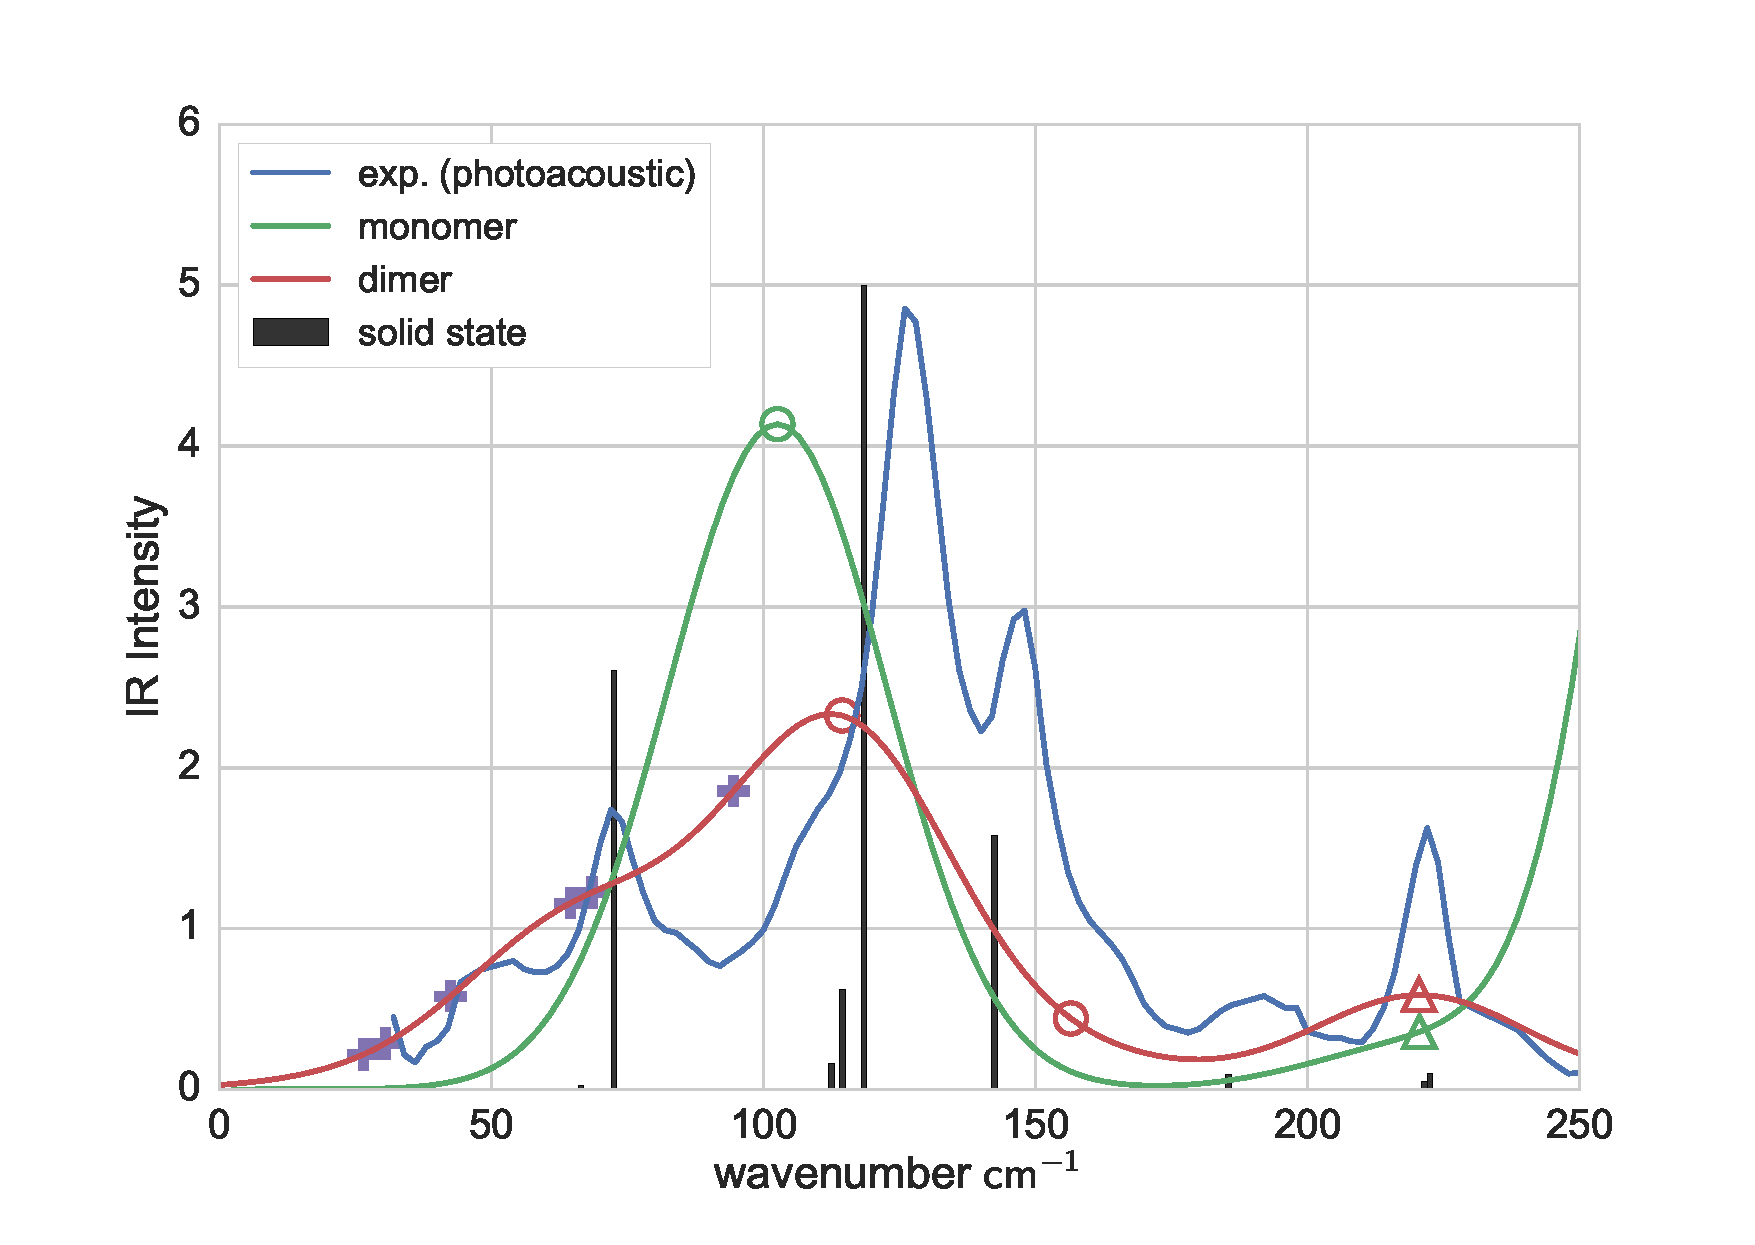
\includegraphics[scale=0.3]{image/carbazole_markers}
 	\caption{Final assignment of the experimental infrared transitions for carbazole. Experimental values are indicated for comparison, and represented with blue lines} \label{figure666}
 \end{figure}

If our previsions turn out to be generalizable for all kind of molecular families and molecules, this could give experimentalists an additional tool of characterisation to identify the presence of systems more or less associated and interacting by means of $\pi$-$\pi$ of $\pi$-H interactions in the solid state. This work is a complement of the results performed in the next chapter concerning the characterisation of the H-bond interactions in asphaltene systems \cite{sodero2016investigation,silva2016molecular}. In this way, we believe to be henceforth capable of disposing all the vibrational pieces of information concerning the three potential types of interactions present in the asphaltenic medium and provide, in this way, experimentalists a way to find out the nature of the interactions present in petroleum fluids and their residues and, to a lesser extent, to identify the chemical nature of oil’s constituents. 
 
 



 \begin{figure}[p]
 	\begin{center}
 		\resizebox{18cm}{!}{
 		\begin{tabular}{c c c}
 			\toprule
 			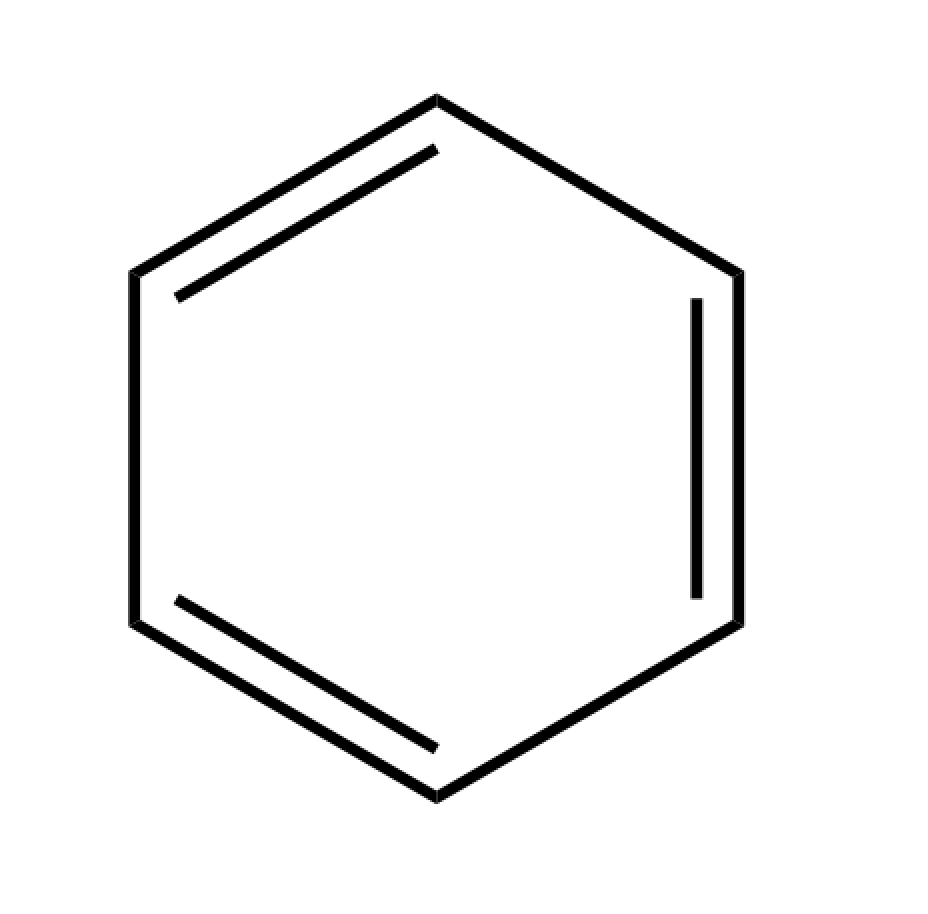
\includegraphics[scale=0.3]{image/benzene} & 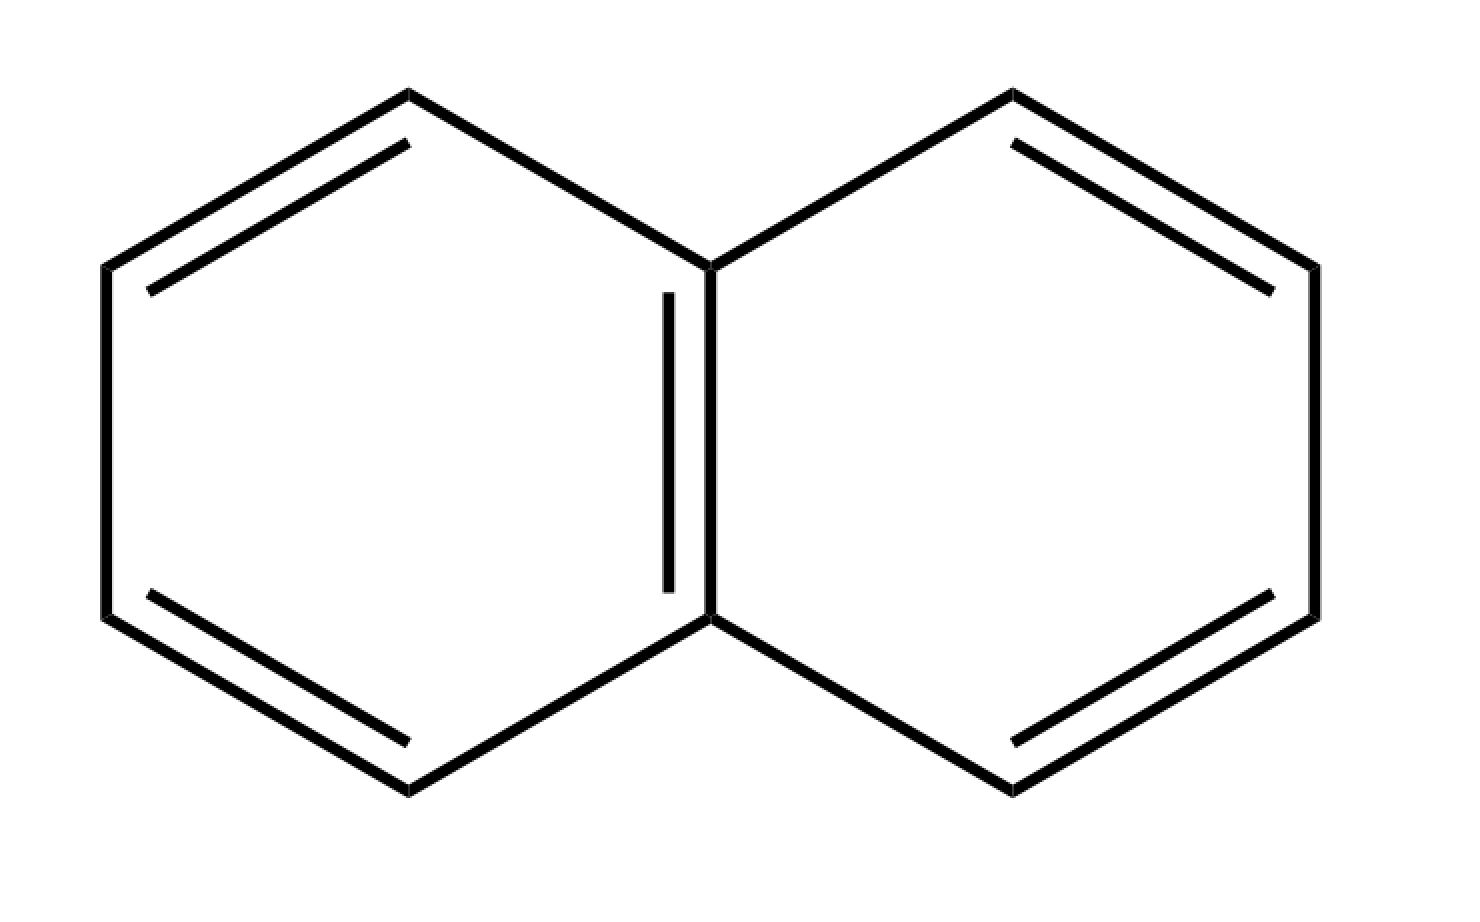
\includegraphics[scale=0.3]{image/naphtalene} & 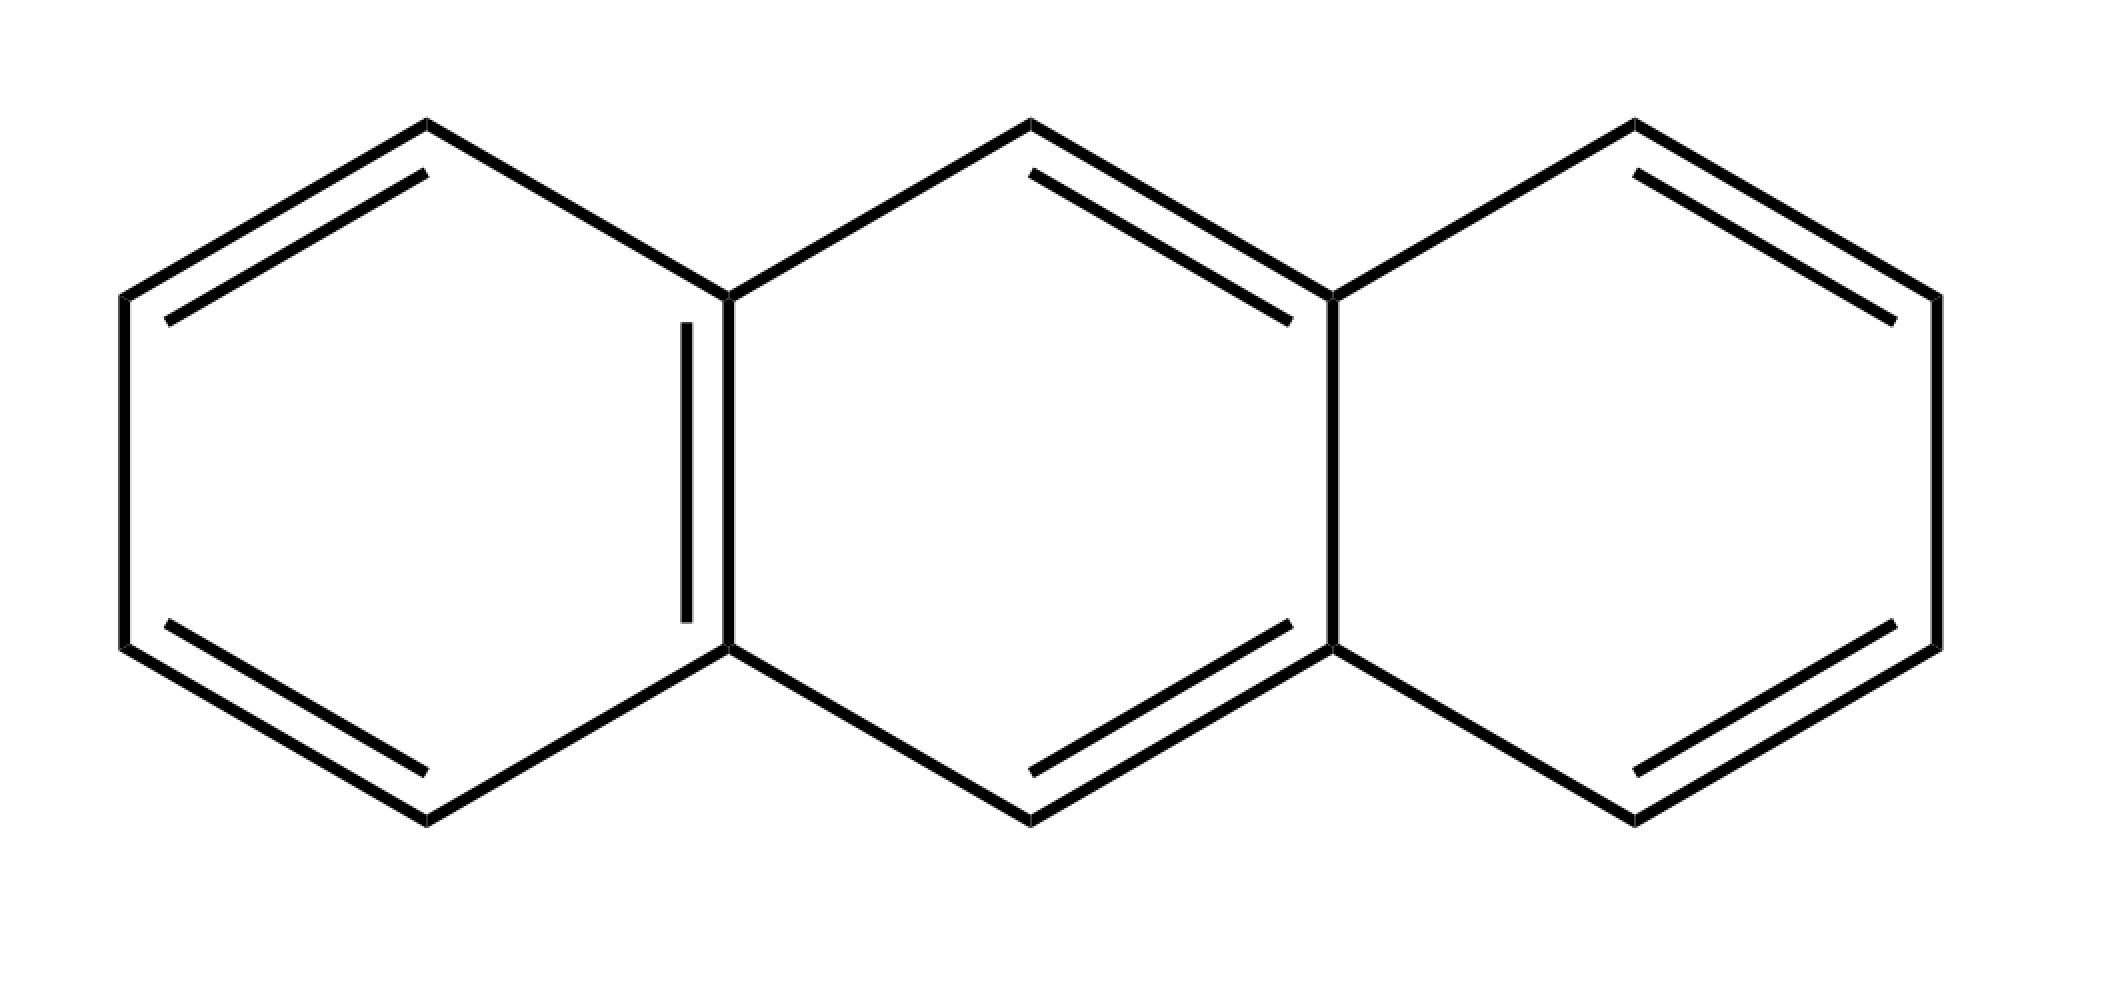
\includegraphics[scale=0.3]{image/anthracene} \\
 			\textbf{Benzene} & \textbf{Naphthalene} & \textbf{Anthracene}\\
 			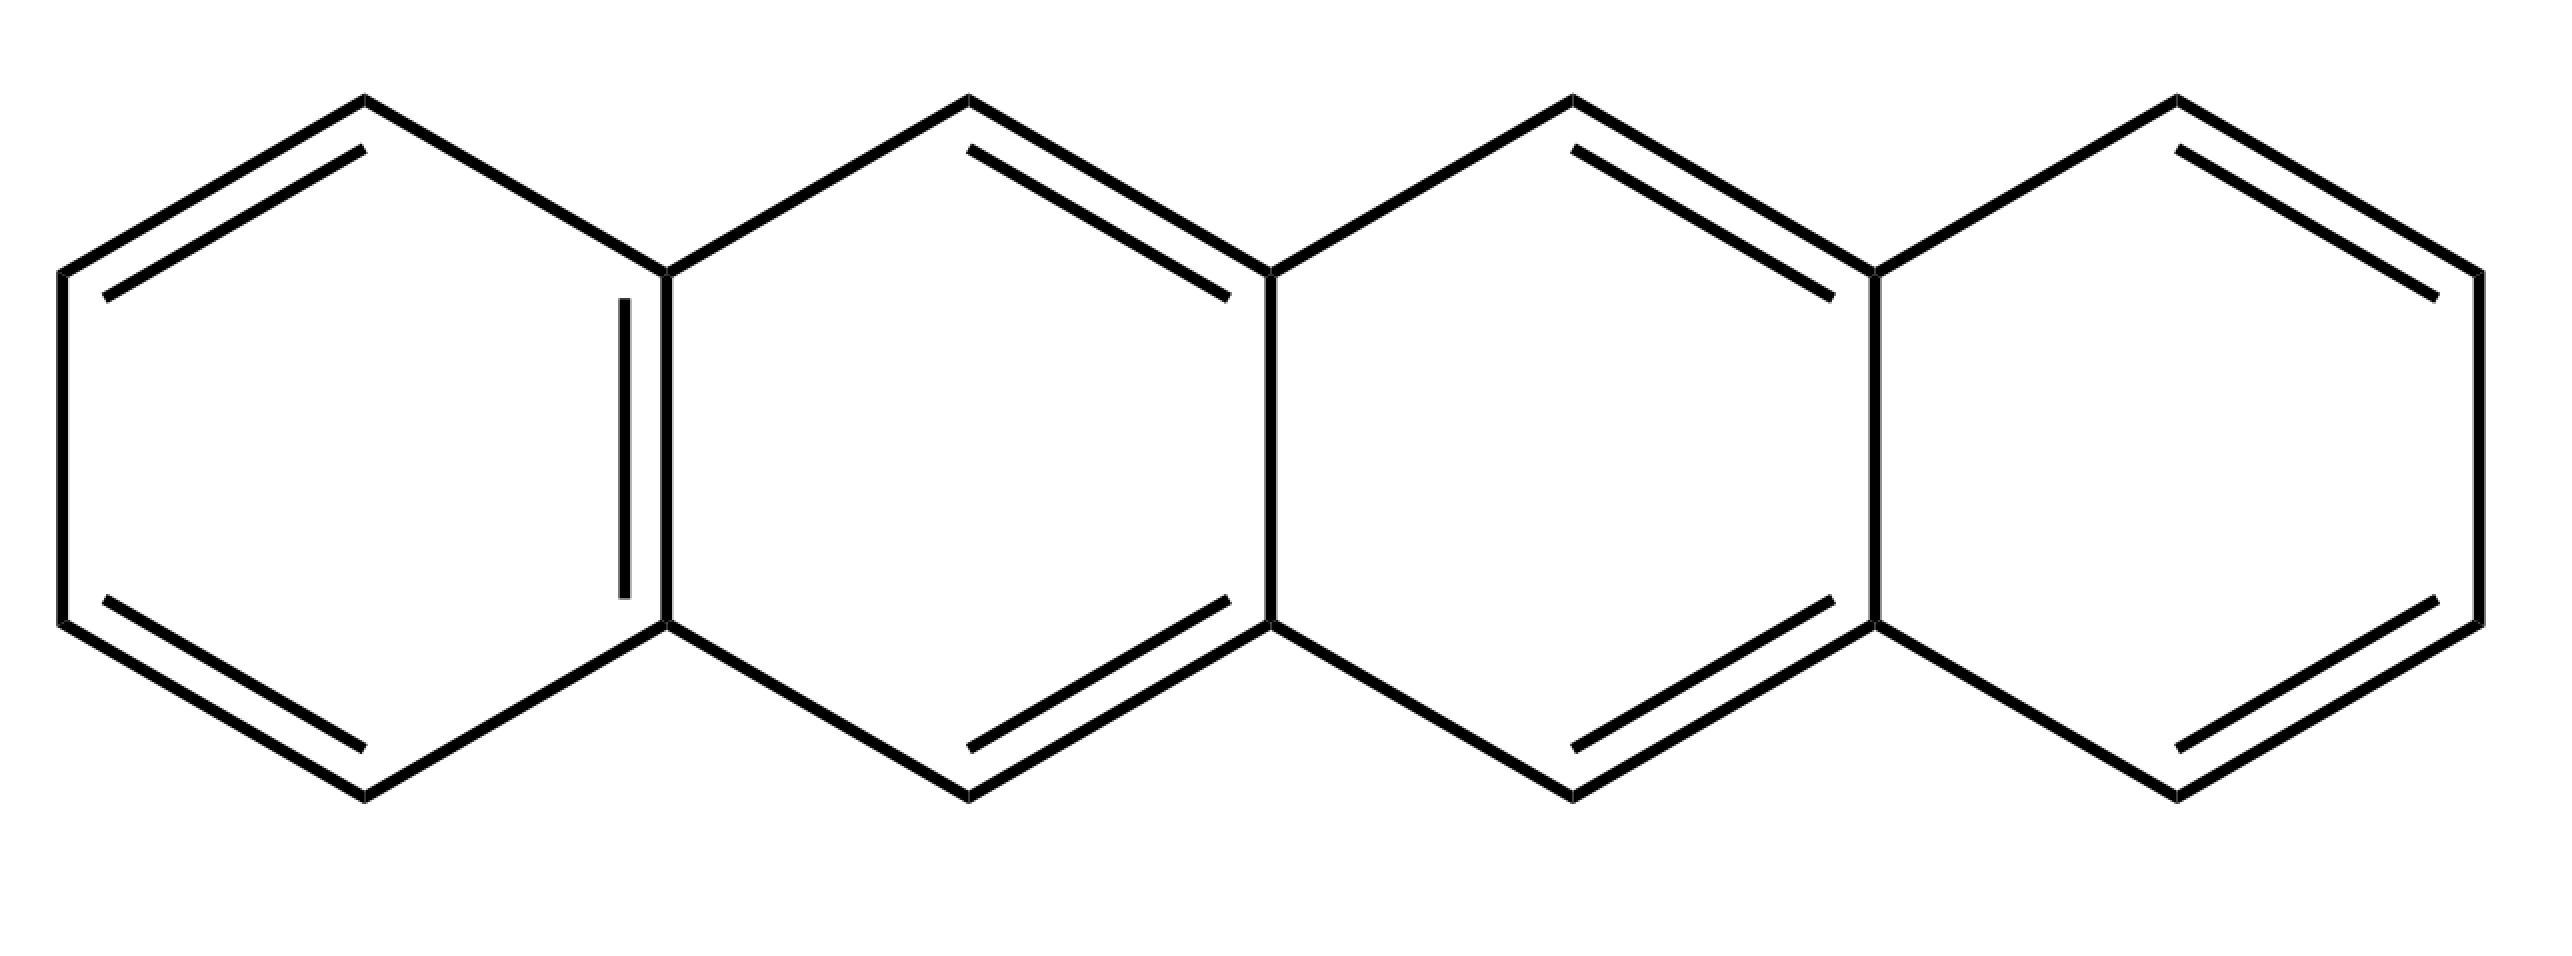
\includegraphics[scale=0.3]{image/tetracene} & & 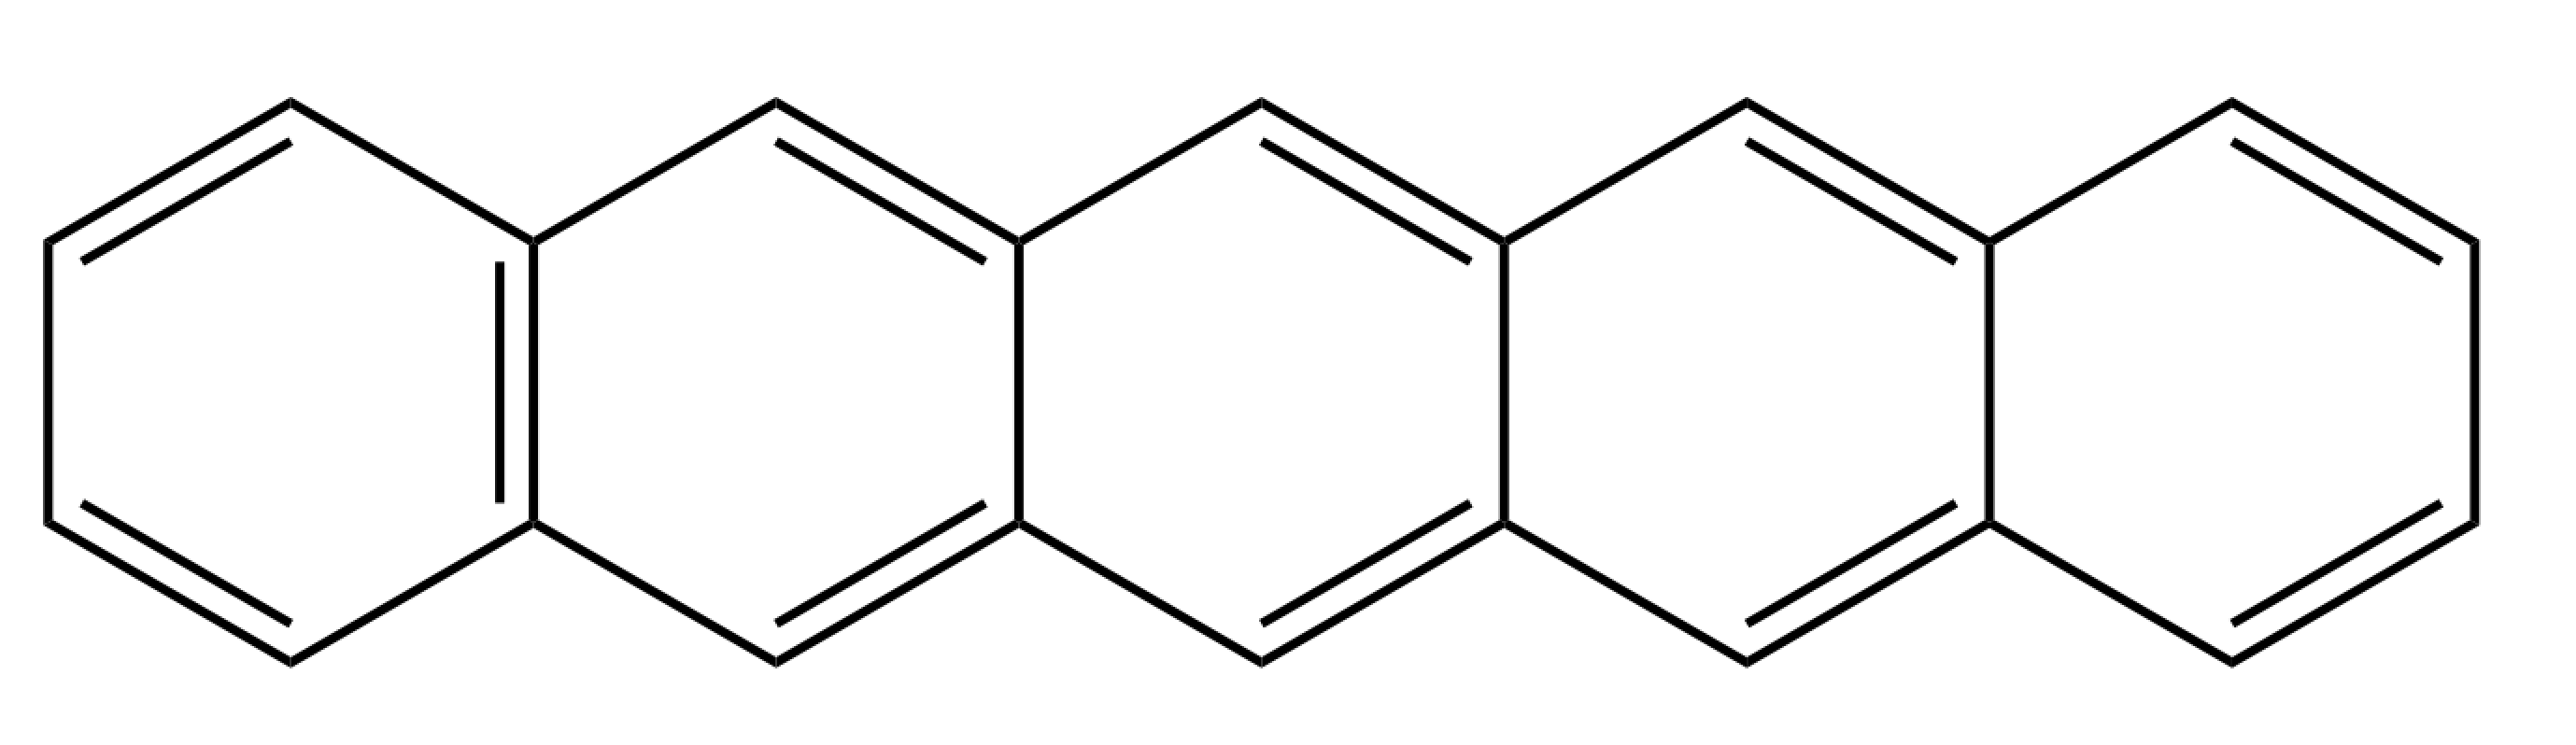
\includegraphics[scale=0.35]{image/pentacene}  \\
 			\textbf{Tetracene} & & \textbf{Pentacene}\\
 			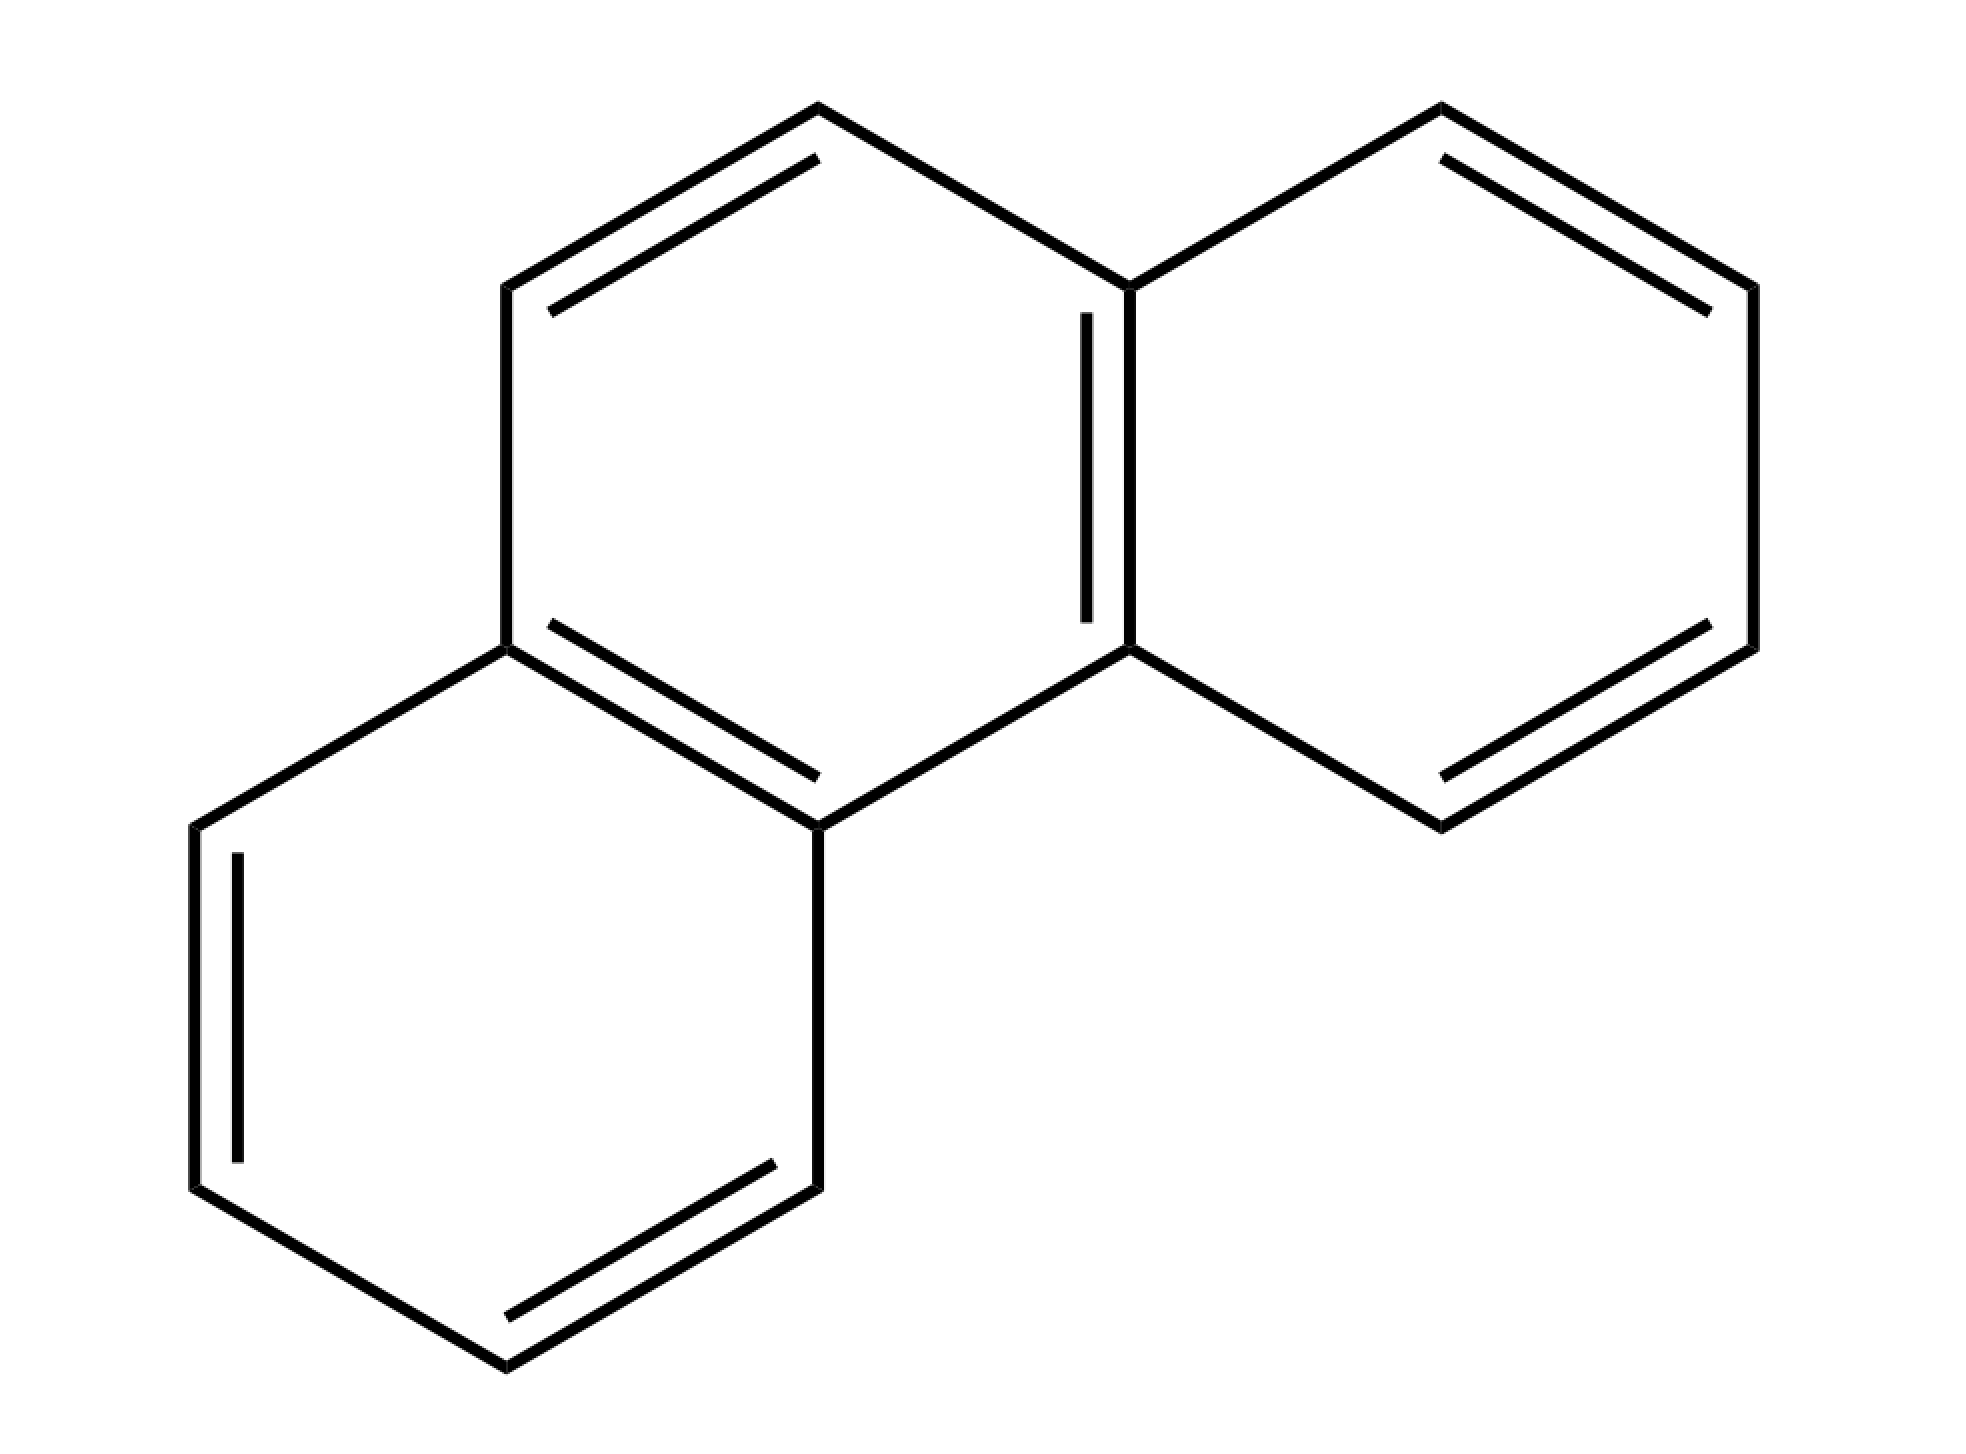
\includegraphics[scale=0.28]{image/phenanthrene} & 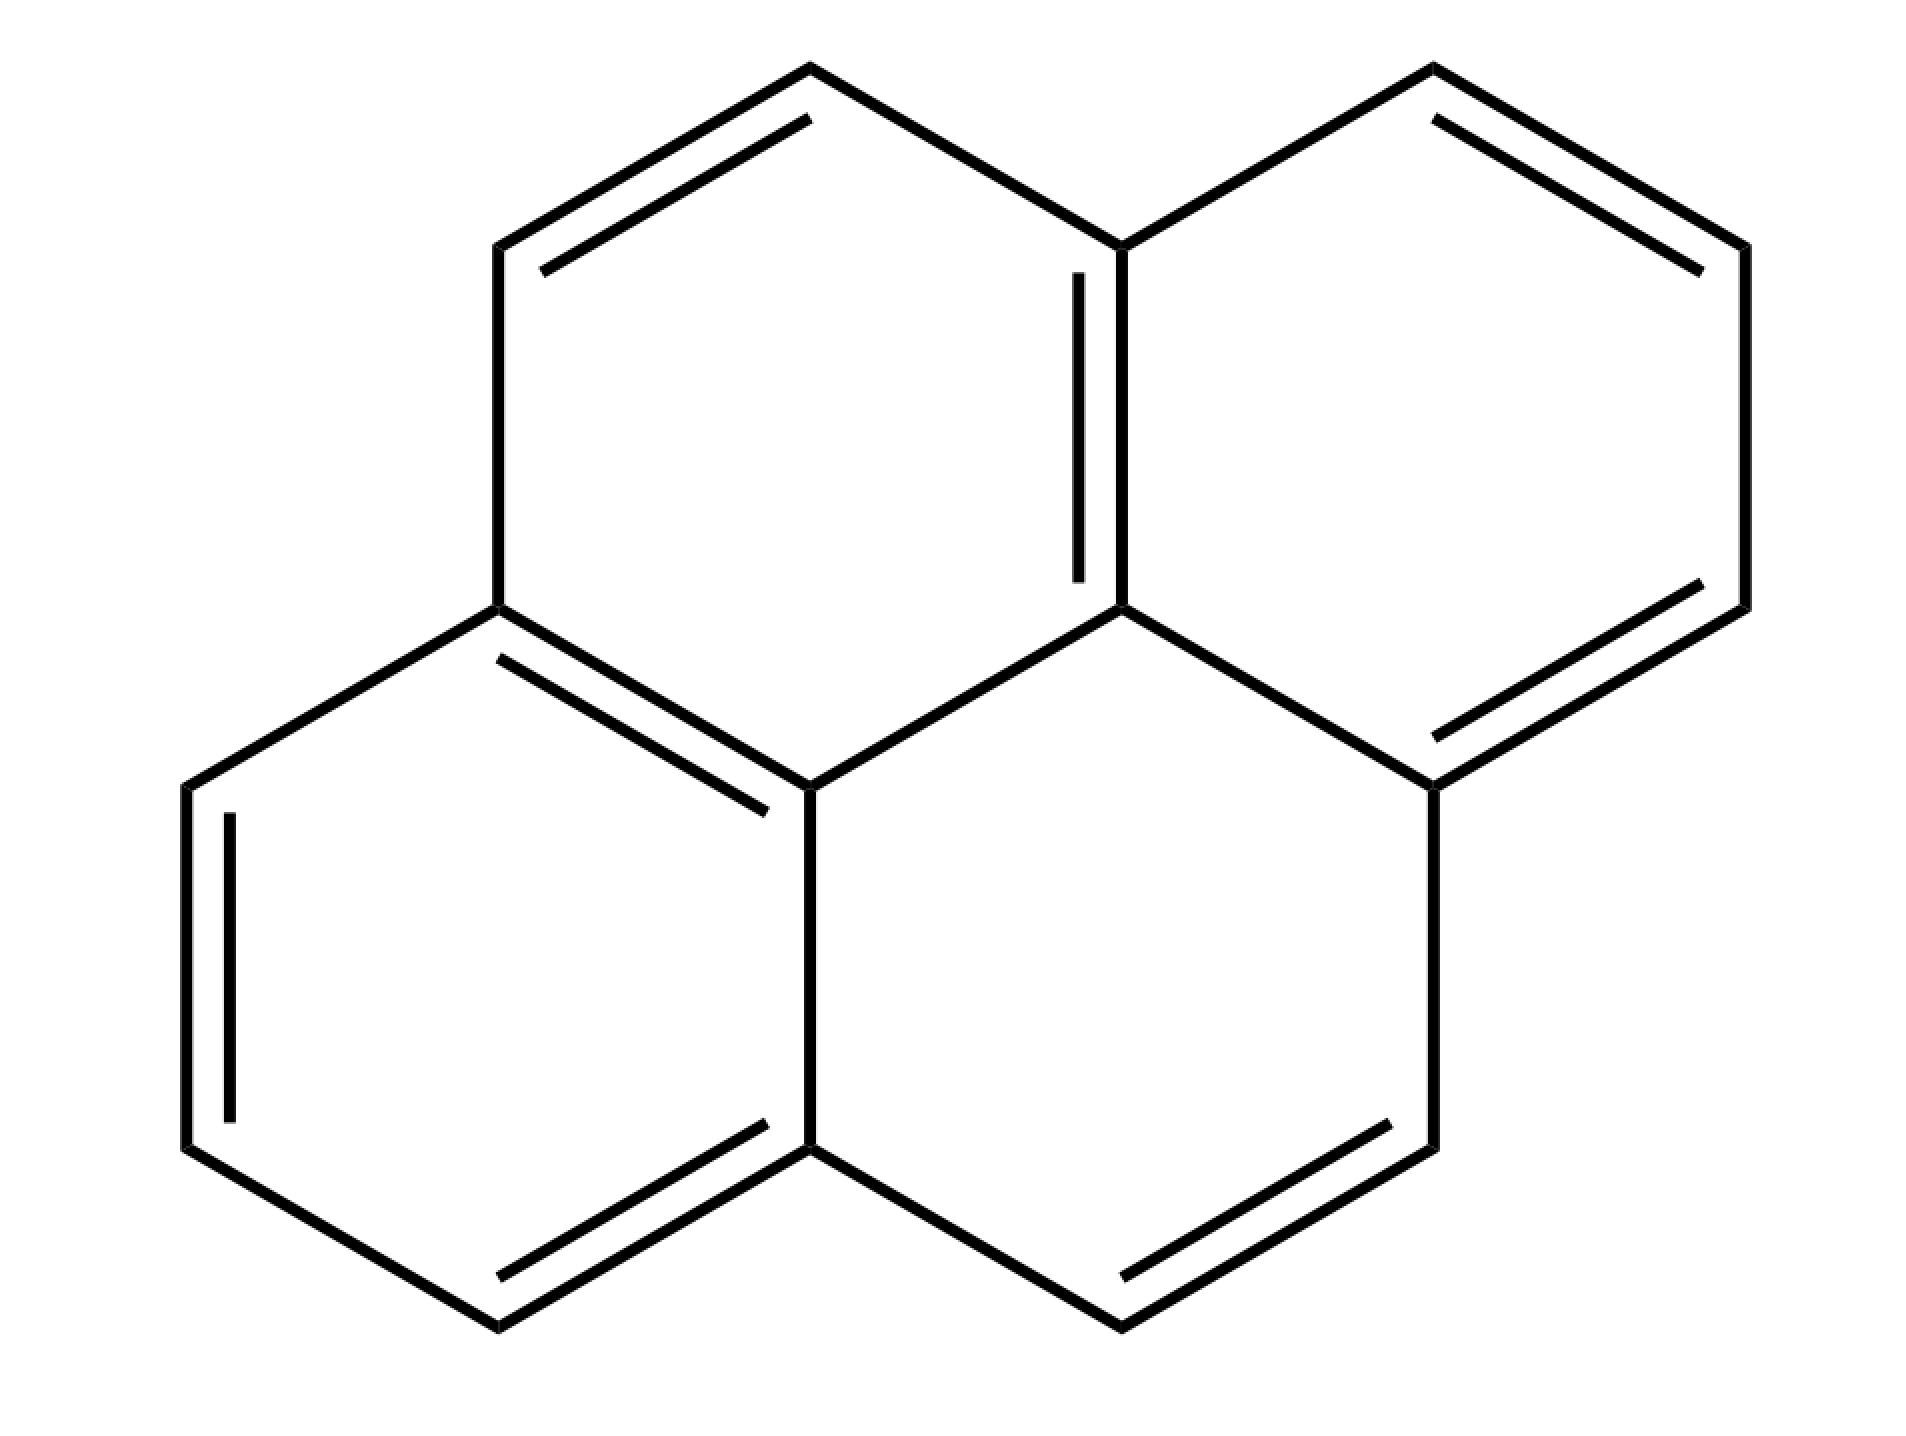
\includegraphics[scale=0.28]{image/pyrene} & 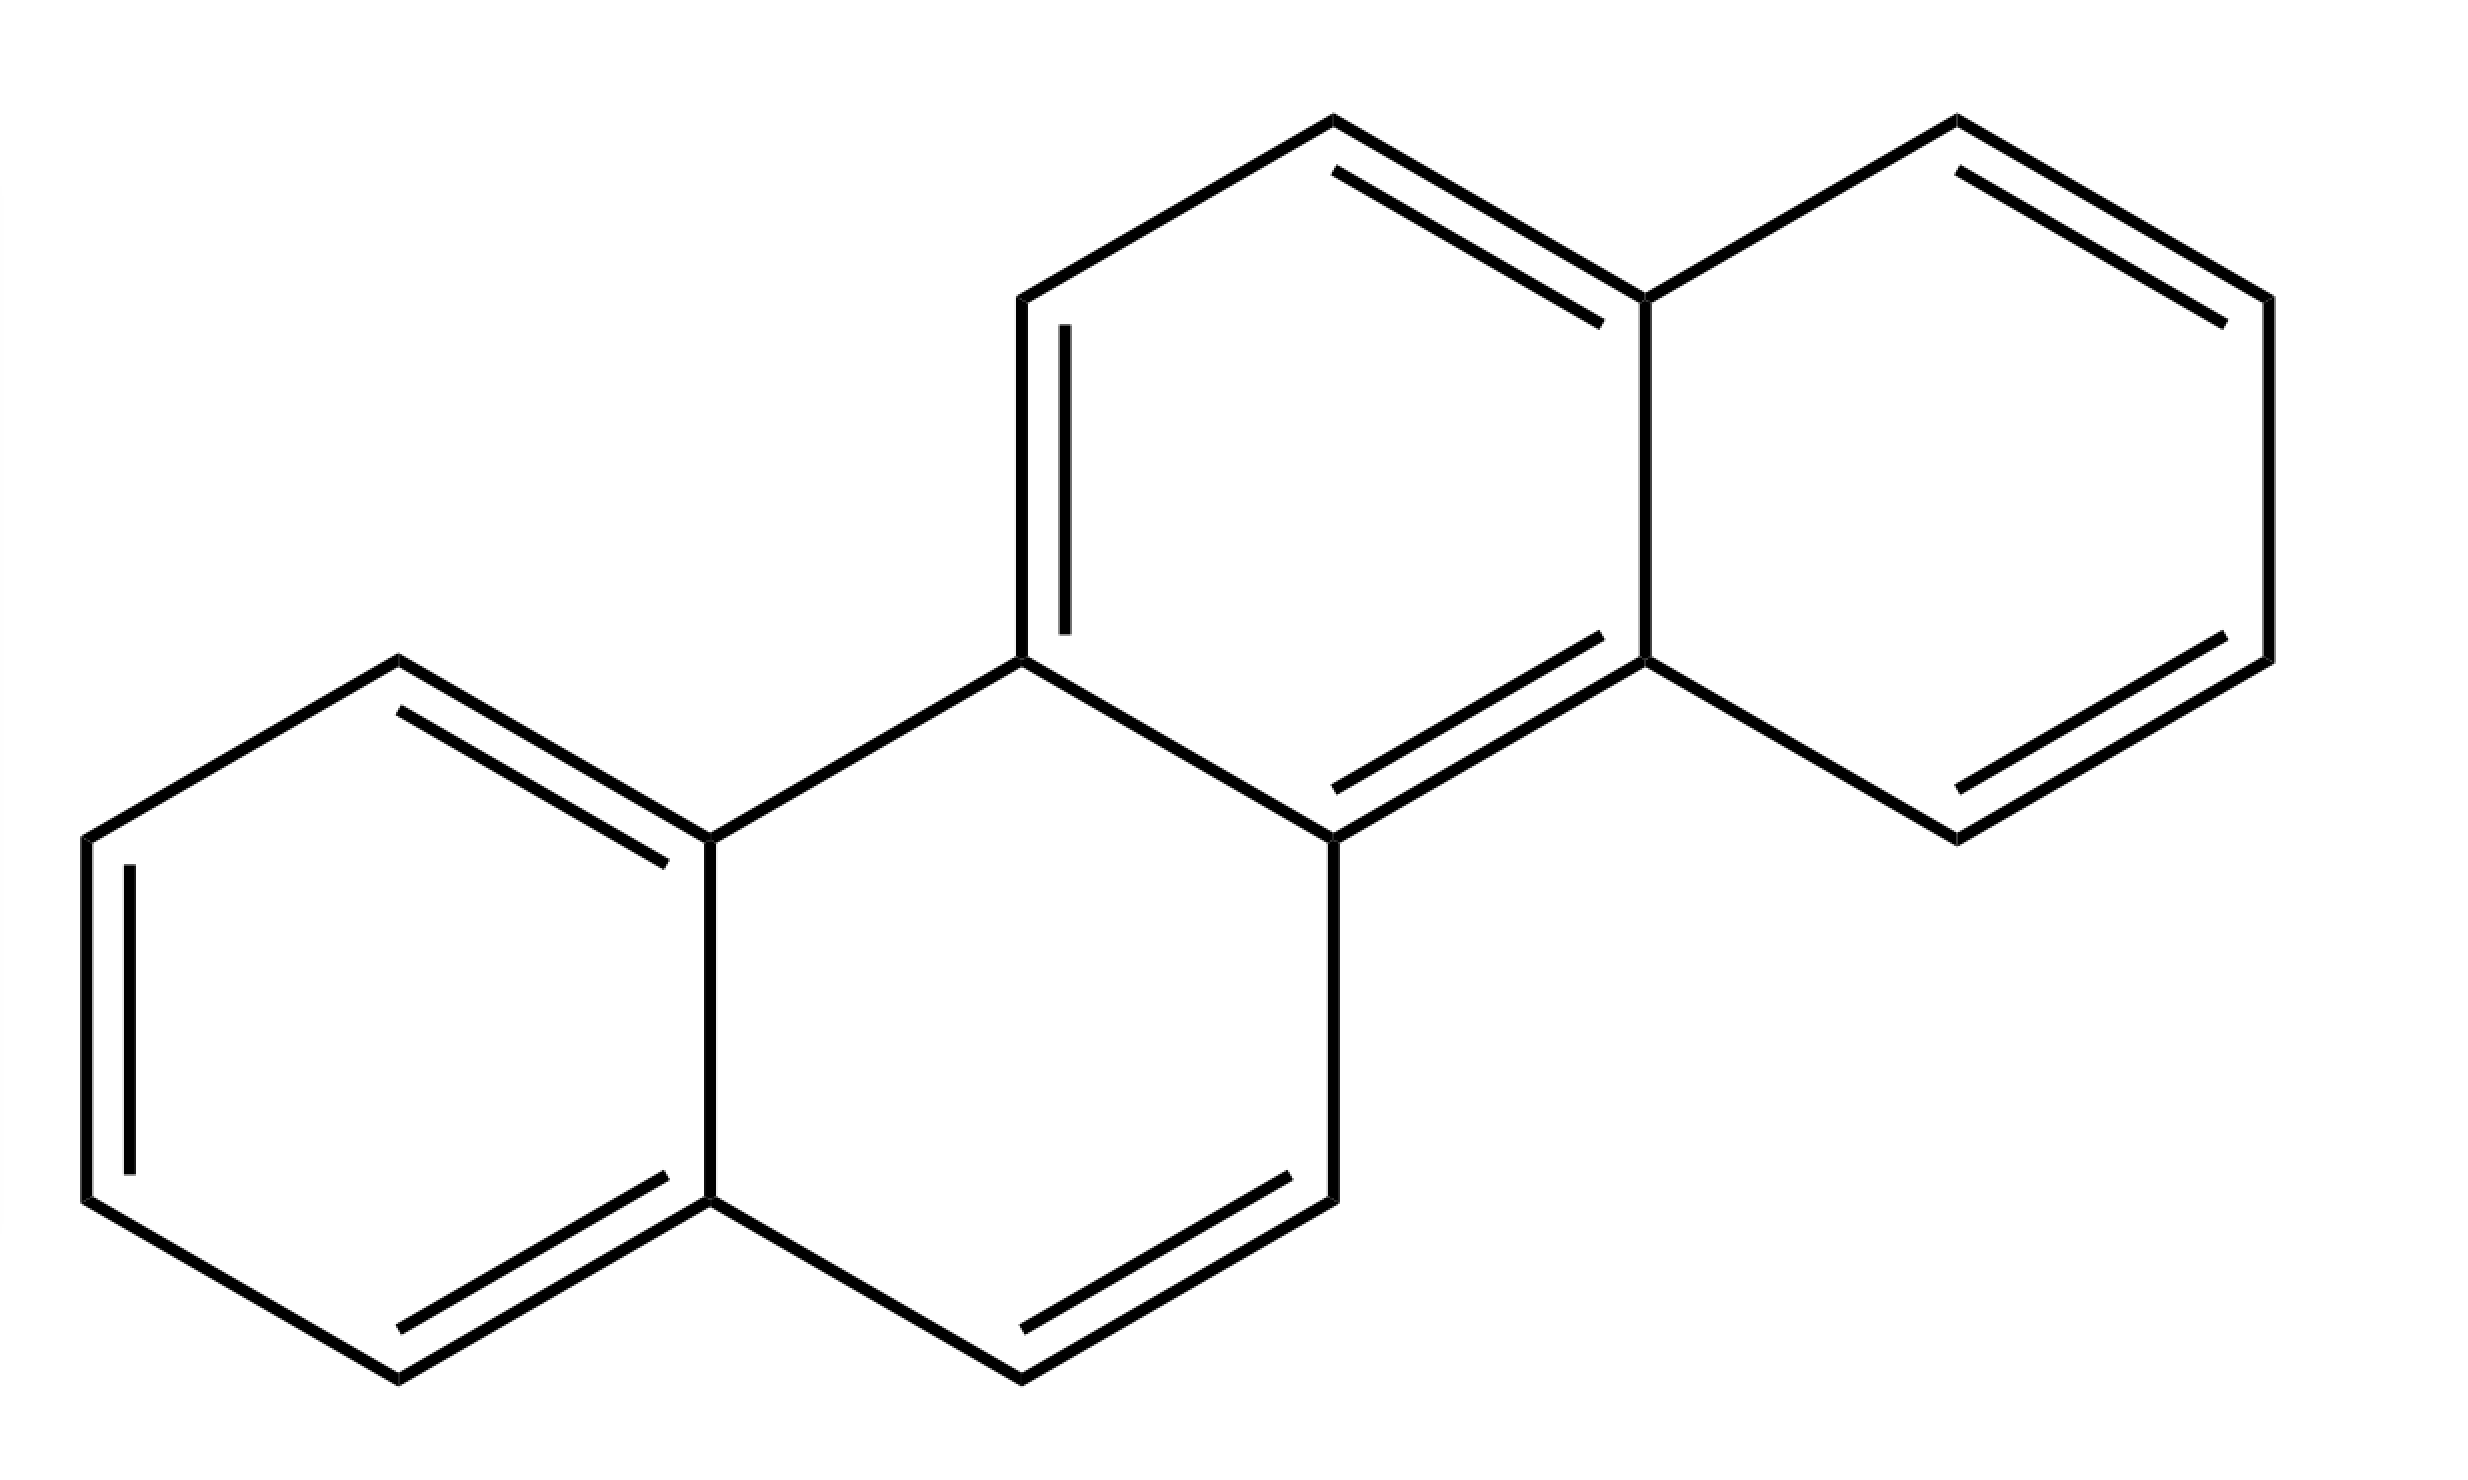
\includegraphics[scale=0.28]{image/chrysene} \\
 			\textbf{Phenanthrene} & \textbf{Pyrene} & \textbf{Chrysene}\\
 			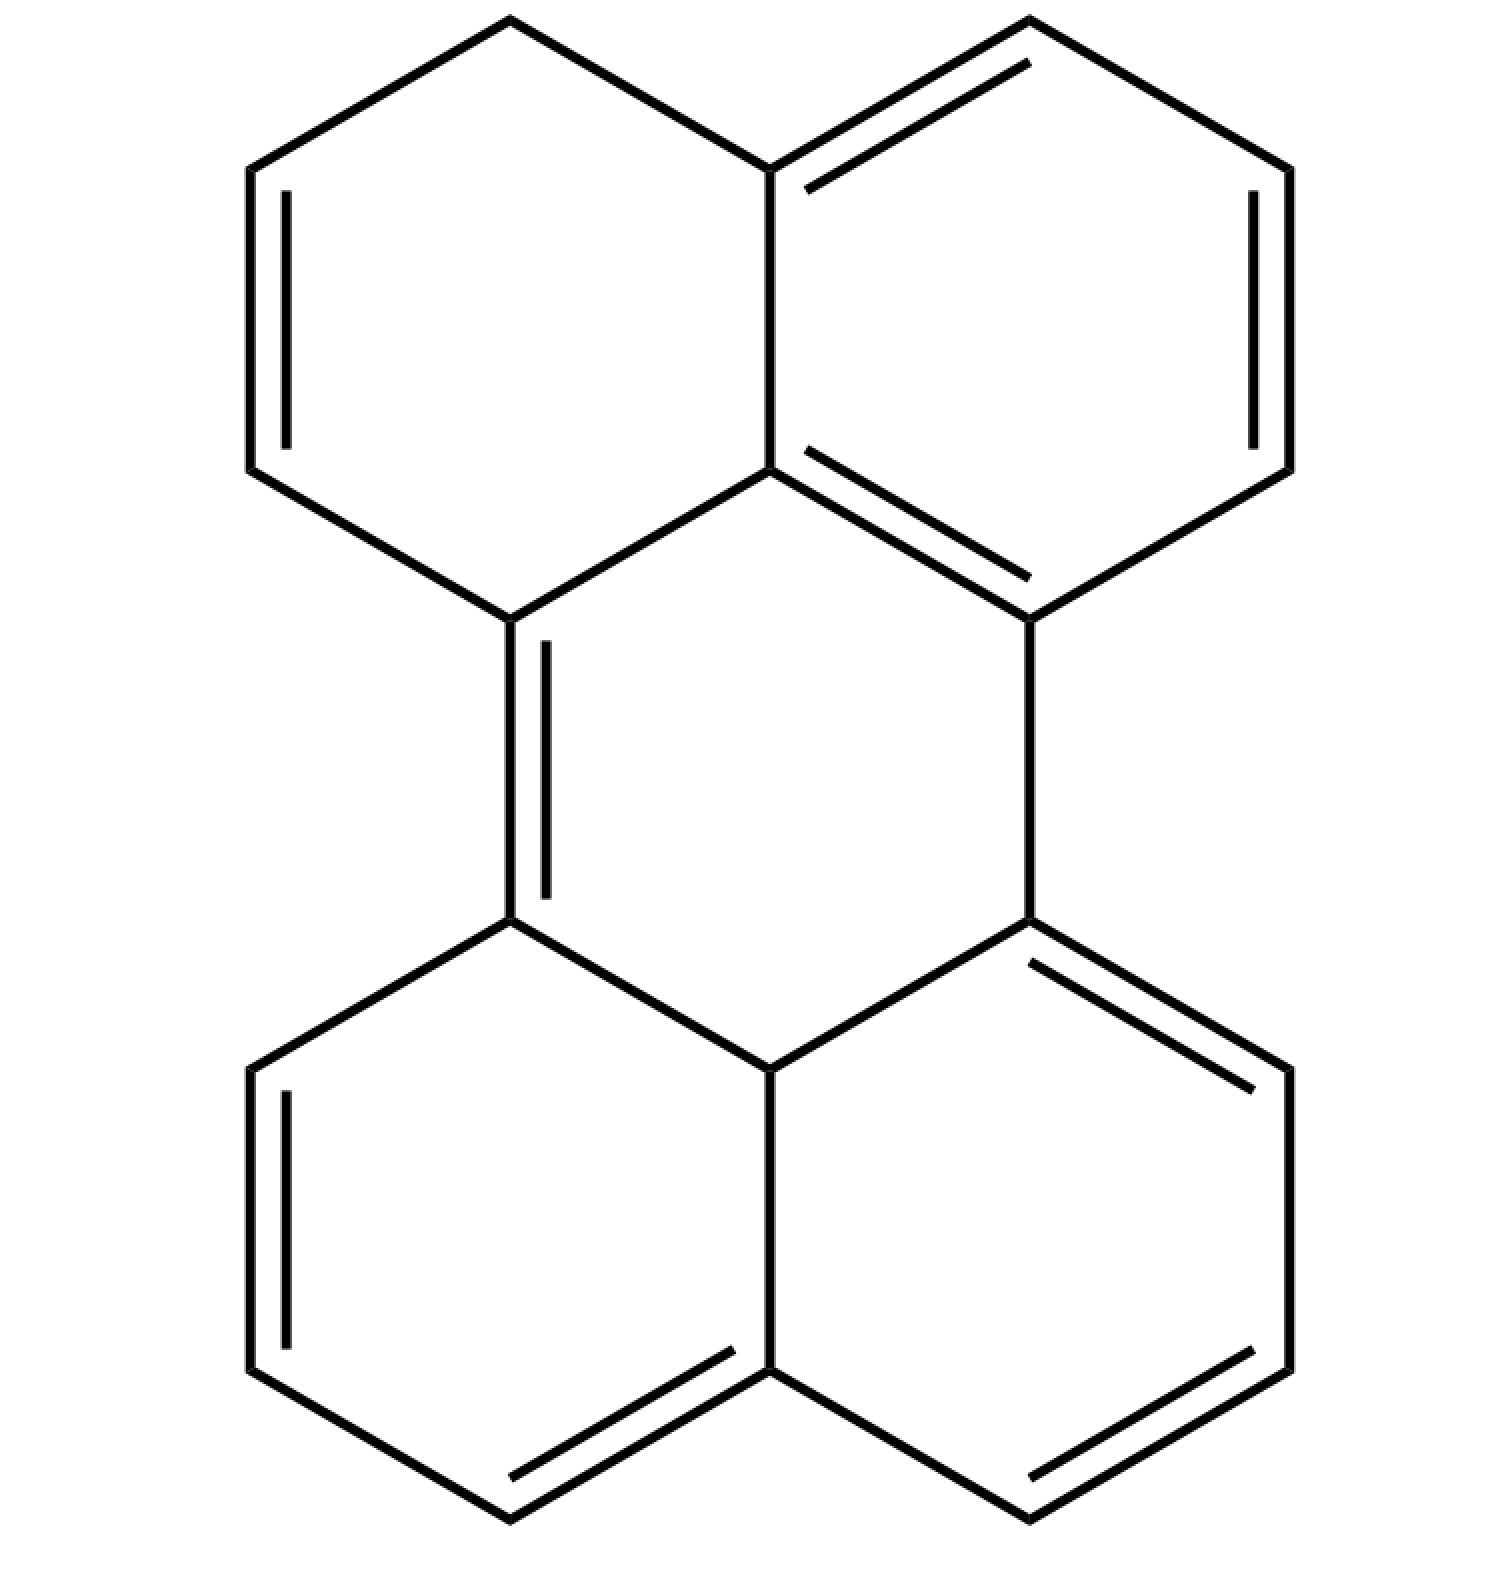
\includegraphics[scale=0.3]{image/perylene} &  &\includegraphics[scale=0.3]{image/fluorene} \\
 			\textbf{Perylene} &  & \textbf{Fluorene}\\
 			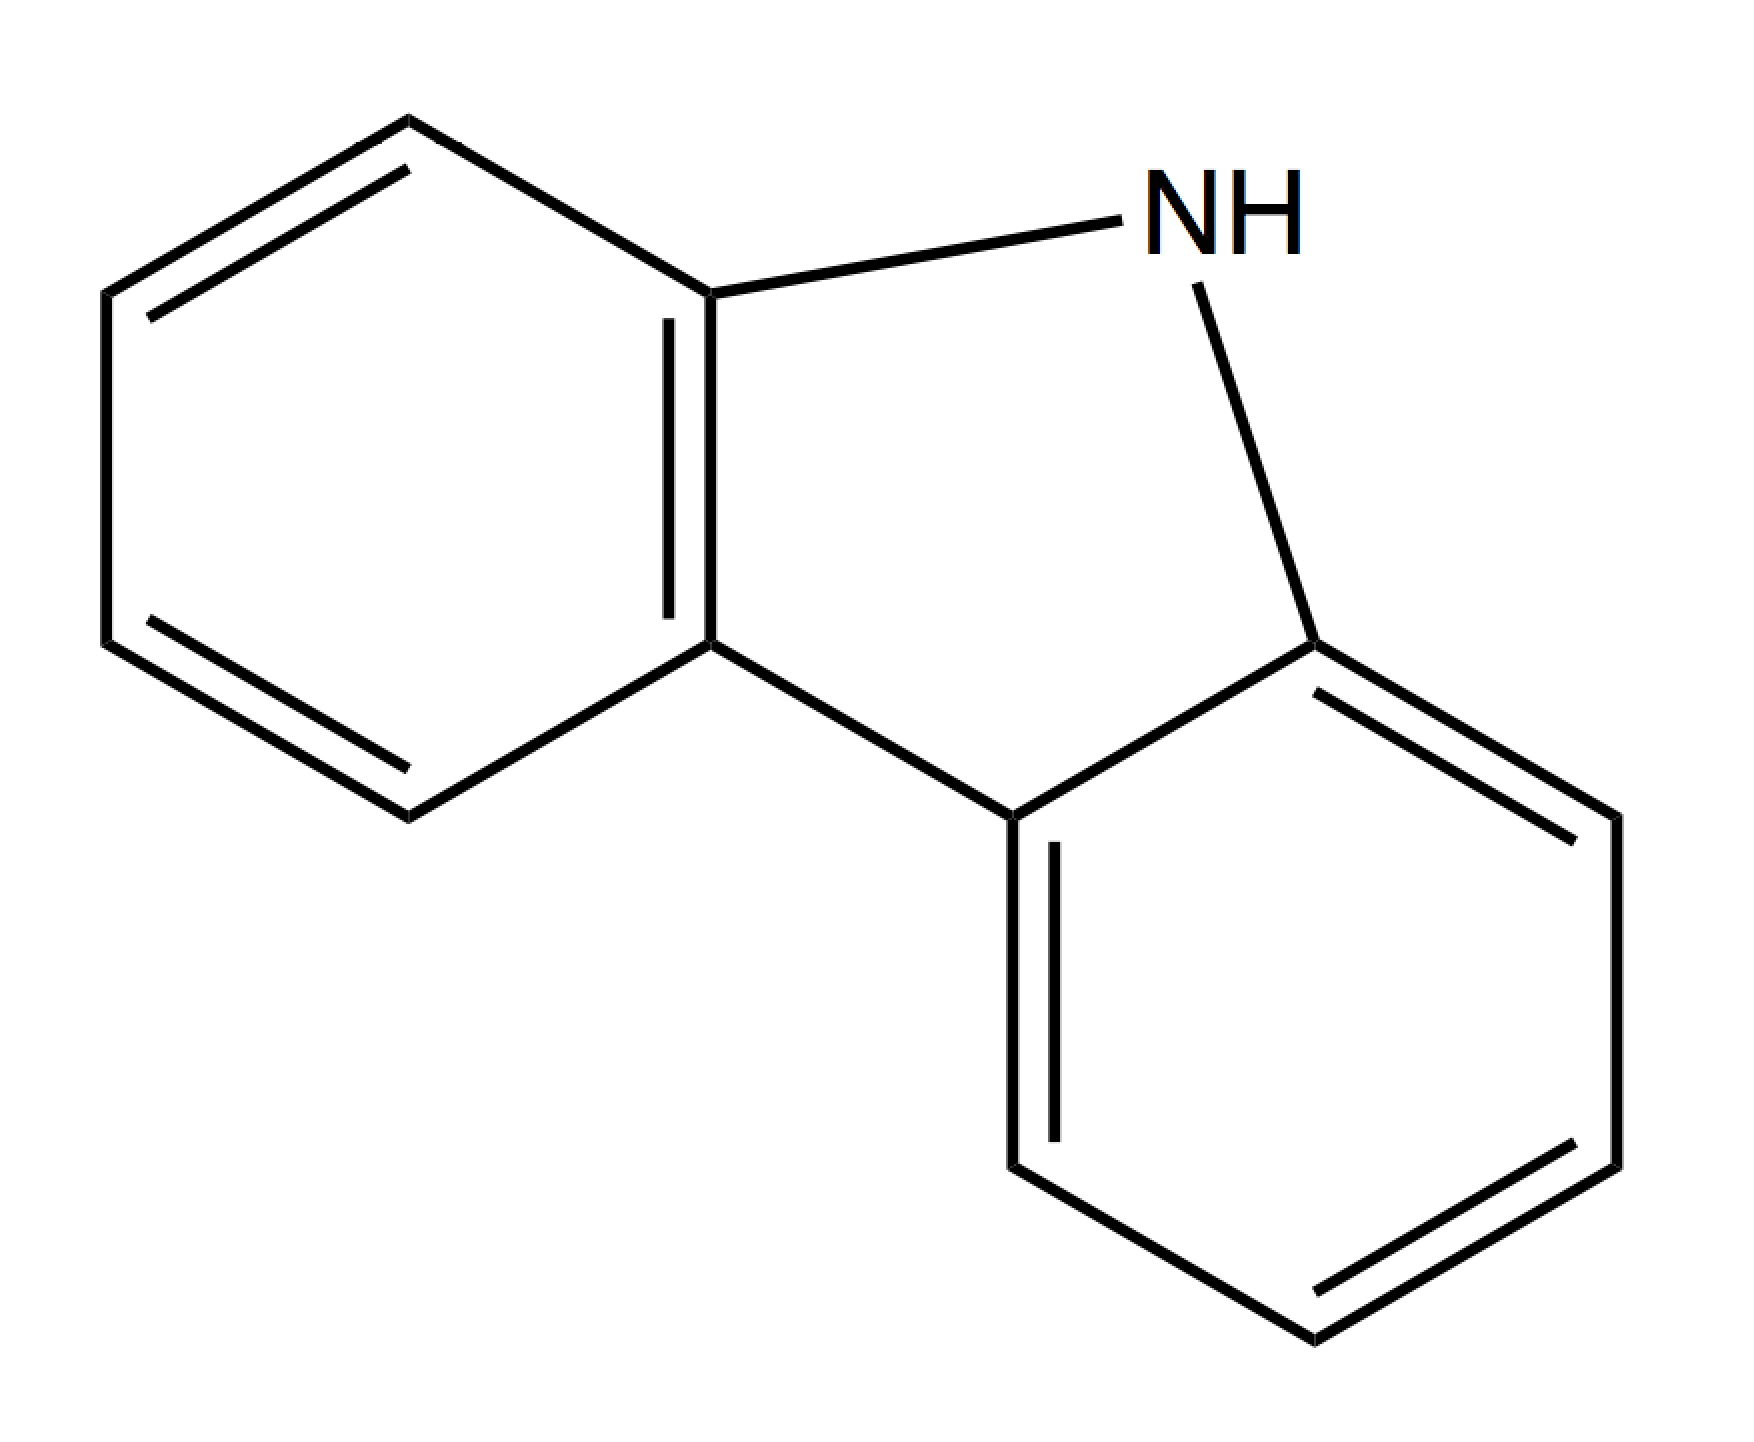
\includegraphics[scale=0.3]{image/carbazole-f} & 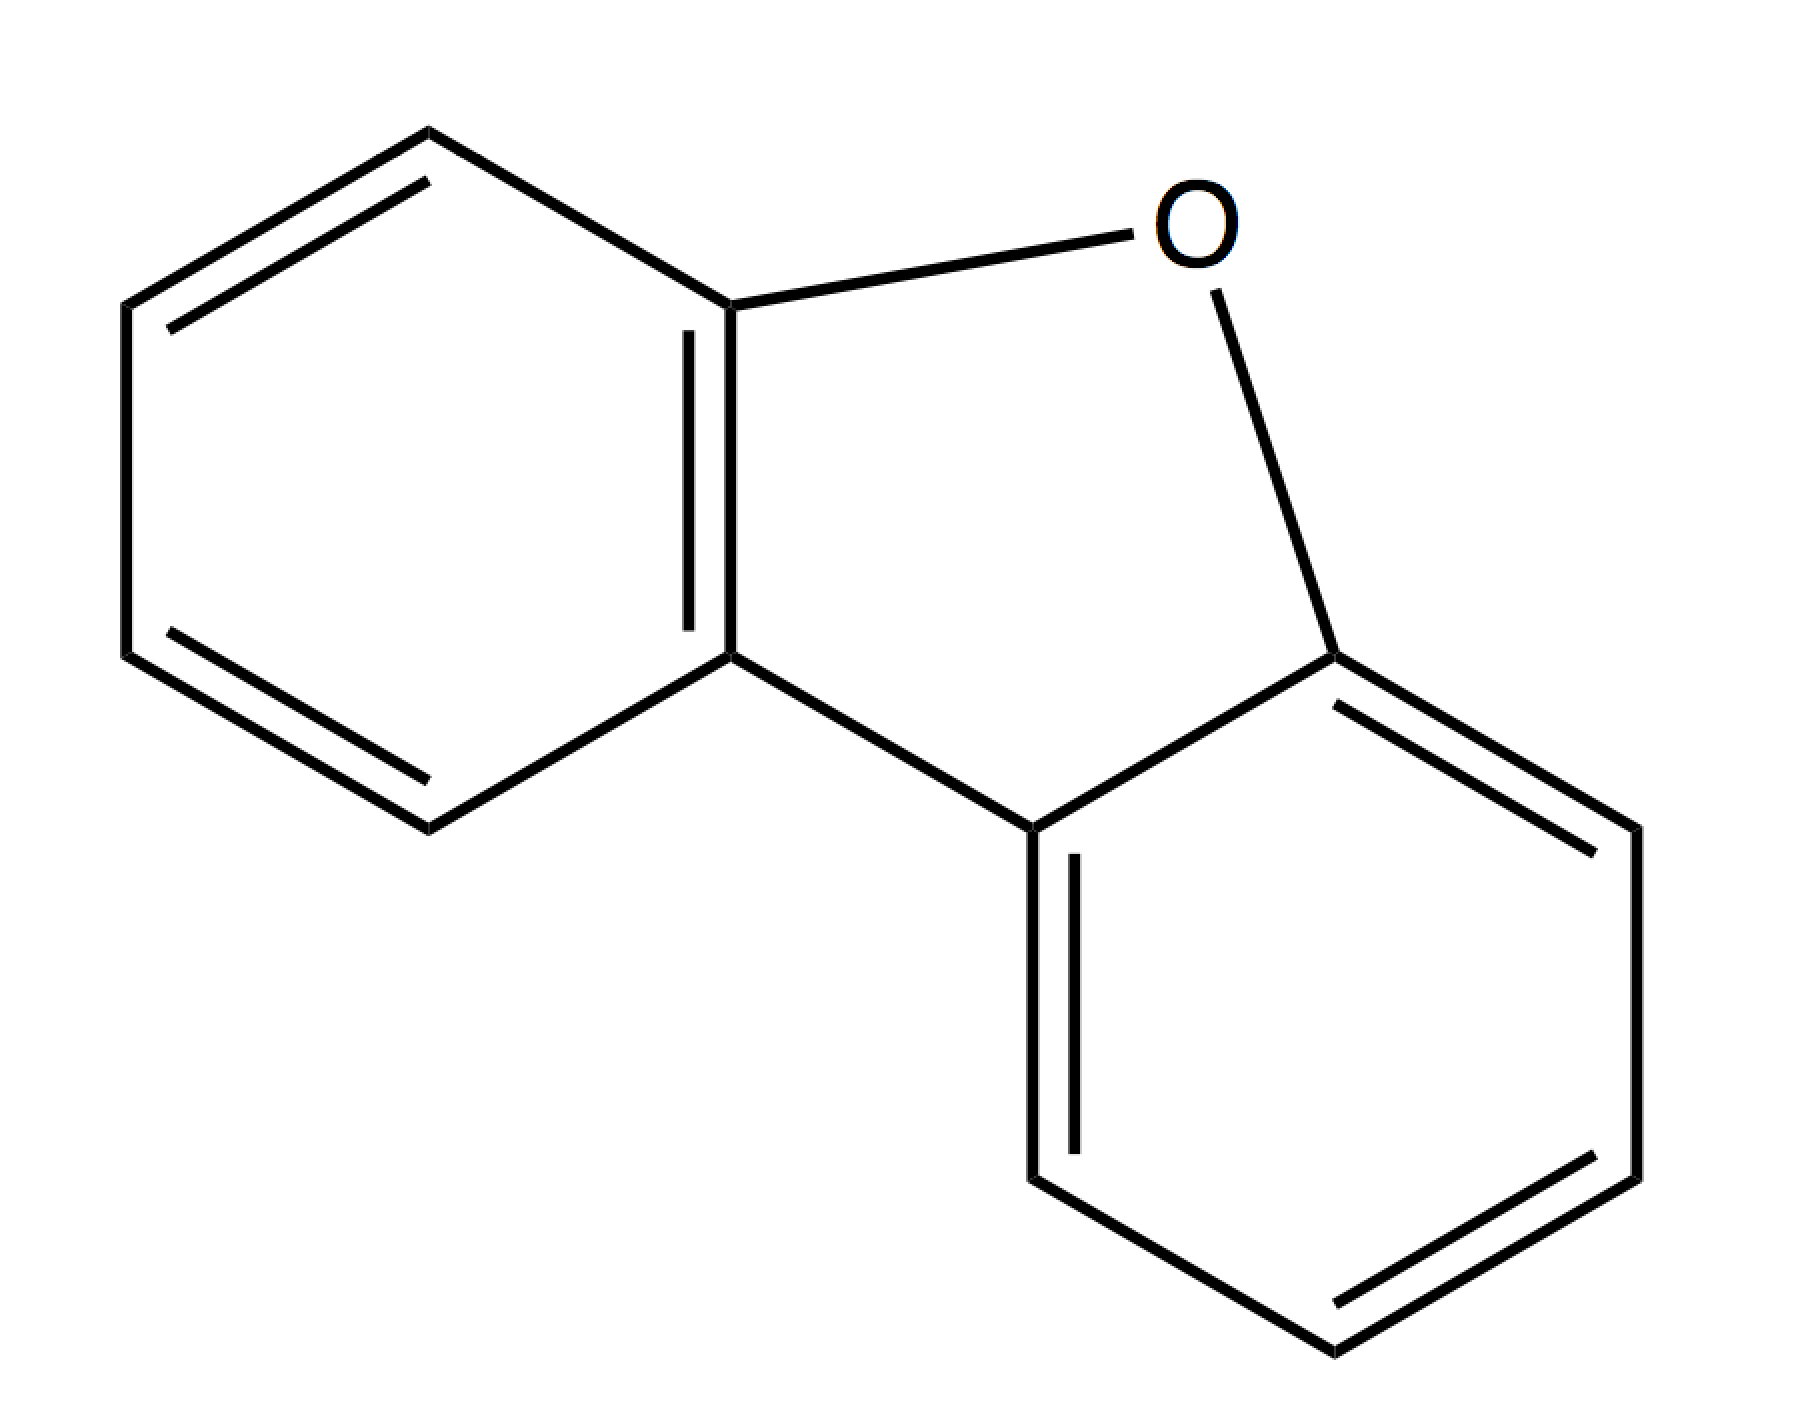
\includegraphics[scale=0.3]{image/dibenzofuran} & 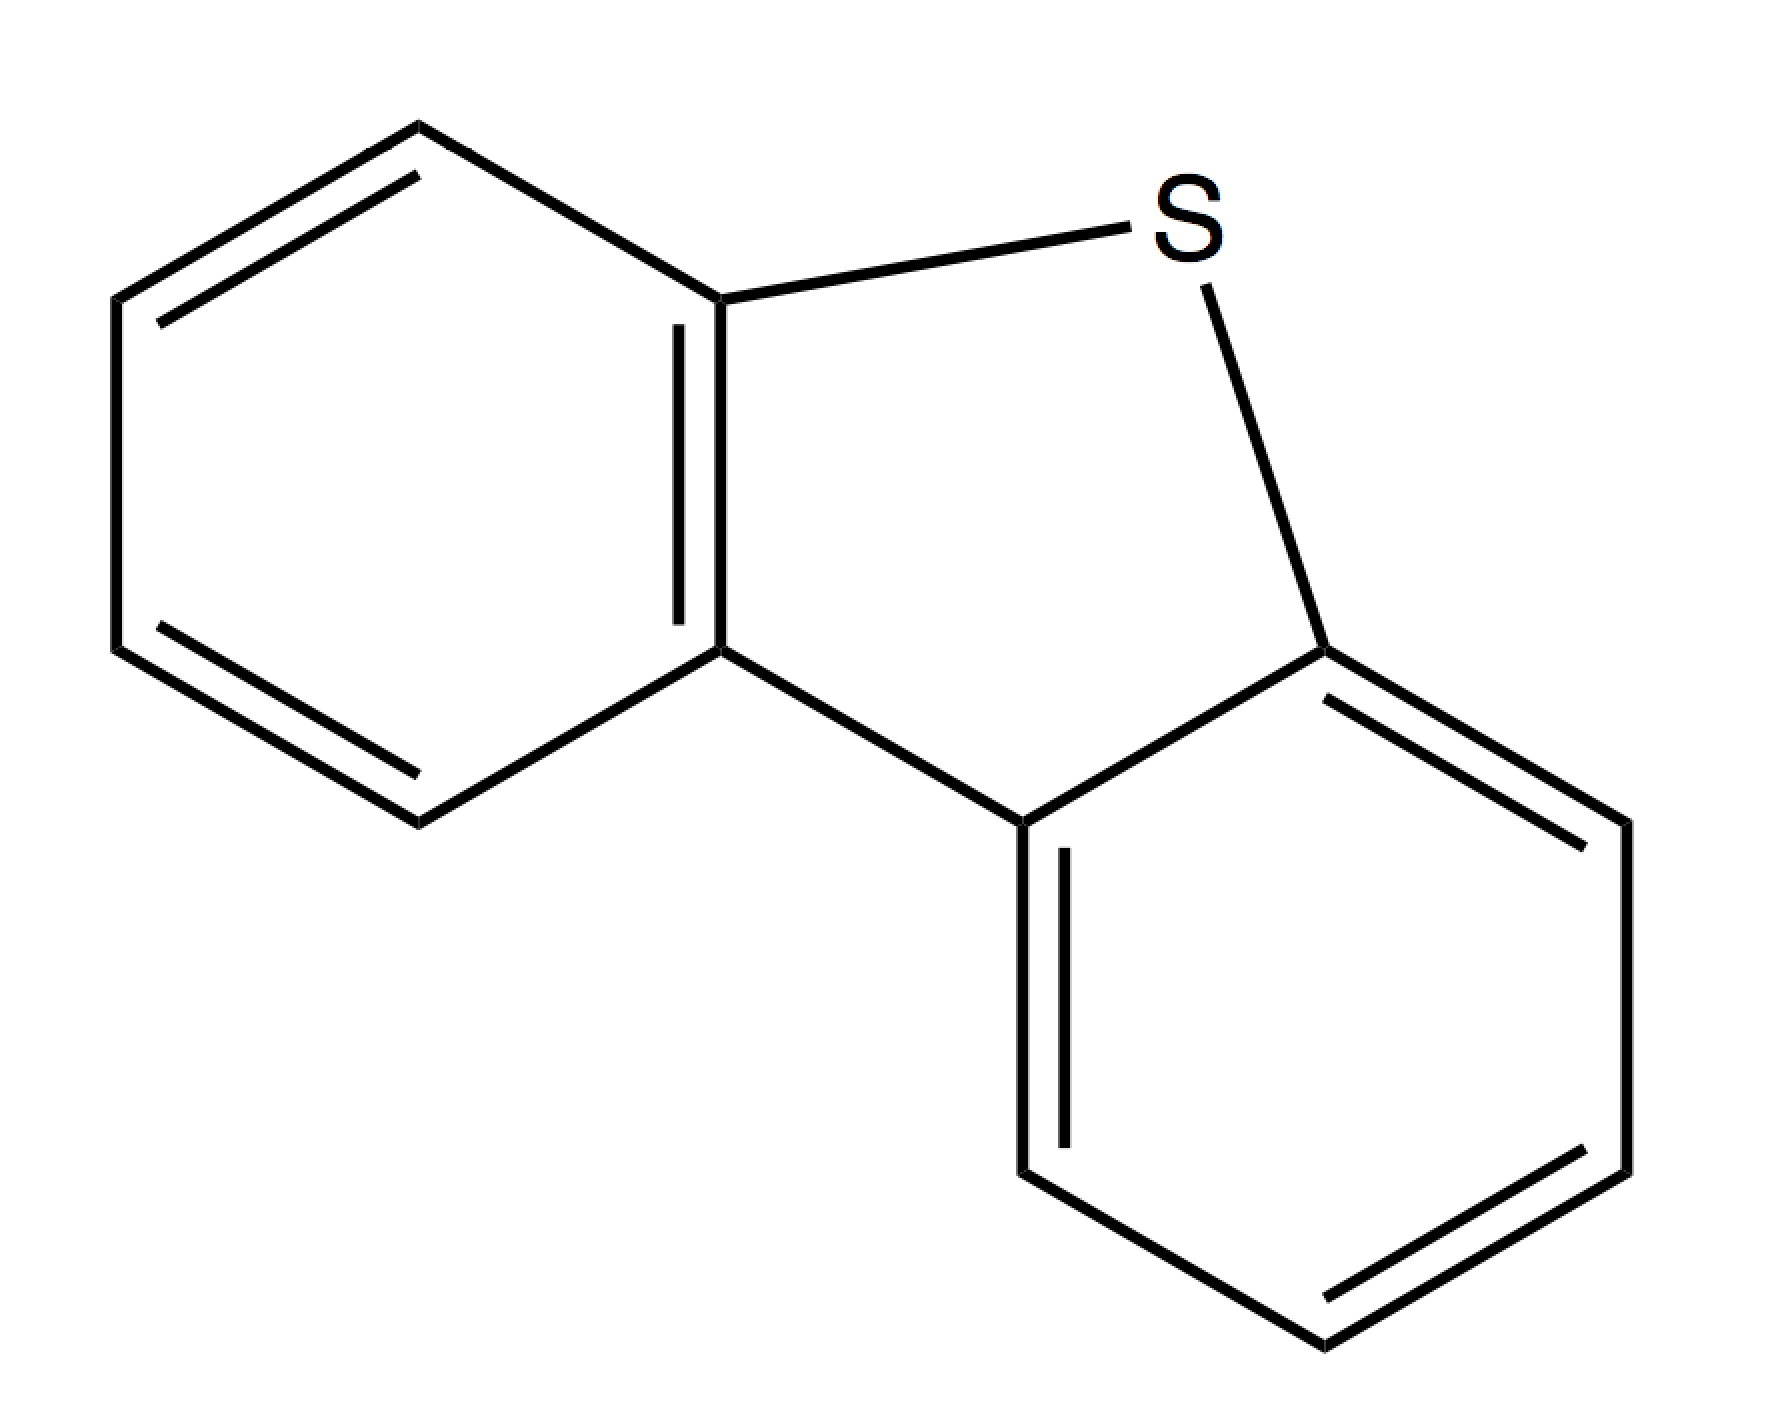
\includegraphics[scale=0.3]{image/dibenzothiophene-f} \\
 			  \textbf{Carbazole} &  \textbf{Dibenzofuran} & \textbf{Dibenzothiophene}\\
 			  \bottomrule
 		\end{tabular}}
 	\end{center}
 	\caption{Molecular structures of studied molecules}
 \end{figure}





